\chapter{Practical Experiments} 
\label{c:Experiments}
After the derivation of the novel deformation energy in \autoref{c:Paper}, this chapter contains some practical experiments to show the robustness of the model and check that each requirement stated in \autoref{ss:stability} is satisfied. The experiments are quasi-static simulations of physical deformations. So, we deform an object in multiple small steps. Quasi-static simulation are well suited for flesh simulations (\cite{teran2005robust}). These simulations are done by posing constraints over the object and then minimizing the deformation energy to find the final position of each vertex.
 
The authors of the paper \textit{\acrshort{snh}} already provided an implementation for an application of their formulated energy\footnote{available at http://graphics.pixar.com/library/StableElasticity/snh\_code.tar.bz2}. Firstly in this chapter, I will examine their implementation and show the results of the experiments with their code. Later, I will present the results of other scenarios, for which I had to change the code accordingly. In the end, I will include a discussion of this new energy formulation considering the results from this chapter.

\section{Technology}
The code the authors provided was written in C++ using the CMake build system\footnote{https://cmake.org/}. It uses the library Eigen (\cite{eigenweb}), version 3.1.2 or newer. The code consists of a core library \verb|cubesim|, which provides the 3D mesh data structure, an implementation of the Stable Neo-Hookean material model, and Newton solvers that minimize the deformation energy over the meshes.

The images in this chapter were taken with the help of OpenFlipper, which is an open-source geometry processing and rendering framework (\cite{mobius2010openflipper}). Furthermore, I used OpenFlipper to create a plugin for some of the experiments. Inside the plugin, I used the integrated library OpenVolumeMesh, which provides a data structure to handle arbitrary polyhedral meshes (\cite{kremer2013openvolumemesh}).

\section{First Experiments}
In this section, I will show the results of the experiments I did with the provided code. The implementation performs a quasi-static simulation of the stretching of a cube. The cube can either be represented by a tetrahedral or a hexahedral mesh. In order to simulate the deformation, the implementation needs a value for each of the two Lamé parameters and a value for defining the desired resolution as input data. In addition, the user has to specify the directory into which the output files should be saved and the material model that should be selected. Since the simulation is quasi-static, the deformation is subdivided into 25 small steps instead of one large step. The output files are 26 static objects in the format .obj. The first file shows the object in its rest state, and the remaining files illustrate the 25 steps of increased deformation. The procedure of the implementation is roughly illustrated in Fig. \ref{fig:procedure}.
\begin{figure}[!htb]
\centering
\begin{tikzpicture}[node distance=2cm]
\node (input) [process] {$\mu$, $\lambda$, resolution};
\node (code1) [decision, right of=input, xshift=1.9cm] {Initialize material model};
\node (code2) [decision, below of=code1, yshift=-0.5cm] {Mesh generation};
\node (code3) [decision, right of=code2, xshift=1cm] {Update boundary conditions};
\node (code4) [decision, right of=code1, xshift=1cm] {Newton solve};
\node (output) [process, right of=code4, xshift=1.9cm] {26 objects};

\draw [arrow] (input) -- node[anchor=south] {Input}(code1);
\draw [arrow] (code1) -- (code2);
\draw [arrow] (code2) -- (code3);
\draw [arrow] (code3) -- (code4);
\draw [arrow] (code4) -- node[anchor=south] {Output}(output);
\end{tikzpicture}
\caption{Illustration of the procedure} \label{fig:procedure}
\end{figure}

I will explain how the implementation works based on an example. For this, I am taking the input variables $\mu = 1.0$, $\lambda = 10.0$ and a resolution of $10.0$. These values for the Lamé parameters result in a Poisson's ratio of 0.46. The command to start the execution for a tetrahedral mesh with these input variables is shown in \autoref{lst:bashCommand}.
\newline
\begin{lstlisting}[language=bash, numbers=none, label=lst:bashCommand, caption=Bash command for executing the code, captionpos=b]
$ ./tetcli 10 stable_neo_hookean 1.0 10.0 output
\end{lstlisting}

Firstly, the implementation initializes the material model Stable Neo-Hookean. Then the generation of the mesh starts. The code creates a cube with $11$ vertices (calculated by resolution + $1$) in each axis. Hence, the cube consists of $11 * 11 * 11 = 1'331$ vertices in total. The number of hexahedra, respectively tetrahedra, are calculated by the following formulas:
\begin{align*}
	&\text{Tet count} = 6 * 10 * 10 * 10 = 6'000 \\
	&\text{Cube count} = 10 * 10 * 10 = 1'000
\end{align*}
Afterwards, the simulation with the $25$ steps of the deformation starts. The code sets two faces of the cube as a boundary condition. A boundary condition in this context denotes a set of fixed vertices. A boundary face is a face for which each vertex is fixed. Fixed vertices already have their final position for the result of the deformation. By updating the boundary conditions, we stretch the cube. That means that these two boundary faces are moved further away from each other along the y-axis. We do this by updating the y-value of the fixed vertices with a new value \verb|newNegativeBoundary| or \verb|newPositiveBoundary| depending on whether the vertex should move in the positive or negative direction along the y-axis. The definition of these two values is shown in \autoref{lst:newBoundary}. The variable \verb|stepNum| is the value of the current step from the $25$ deformation steps. For each step the stretching should increase. To achieve this, we use the variable \verb|stepDelta|. Its value is equal to $0.1$ and stays constant for these first experiments.
\begin{lstlisting}[language=C++, numbers=none, label=lst:newBoundary, caption=Updating y-coordinates of vertices, captionpos=b]
const double newNegativeBoundary = -1.0 - stepNum * stepDelta;
const double newPositiveBoundary = 1.0 + stepNum * stepDelta;
\end{lstlisting}
After the new positions of the fixed vertices are declared, the \verb|TetNewtonSolver|, respectively \verb|CubeNewtonSolver|, is used to minimize the strain energy over the mesh and determine the position of the remaining vertices. The optimization process will be further explained in \autoref{s:optimization}. Finally, the mesh is saved in a .obj file in the directory \verb|output|. 

Tables \ref{table:default_tet} and \ref{table:default_hex} show, the total number of Newton iterations that had to be performed by the solver to reach an acceptable solution. The number of iterations are listed for a specific step number or an interval of step numbers. For example, step number 1 to 10 each required 3 Newton iterations. The step number denotes in which of the 25 steps of deformation we currently are. In \autoref{lst:newBoundary} I called this variable \verb|stepNum|. The amount of iterations increases with increasing step number. This increase is not surprising, since the deformation is also increased with each step resulting in more calculations.

\begin{table}[!htbp]
\parbox{.45\linewidth}{
\centering
\begin{tabular}{ | l | l |}
\hline
\textbf{Step number} & \textbf{Iterations} \\ \hline
1-10 & 3 \\ \hline
11-21 & 4 \\ \hline
22-25 & 5 \\ \hline
\end{tabular}
\caption{Newton iterations for a tetrahedral mesh}
\label{table:default_tet}
}
\hfill
\parbox{.45\linewidth}{
\centering
\begin{tabular}{ | l | l |}
\hline
\textbf{Step number} & \textbf{Iterations} \\ \hline
1-7 & 4 \\ \hline
8-14 & 5 \\ \hline
15-18 & 6 \\ \hline
19-22 & 7 \\ \hline
23-25 & 8 \\ \hline
\end{tabular}
\caption{Newton iterations for a hexahedral mesh}
\label{table:default_hex}
}
\end{table}

The images in Fig. \ref{fig:stretchtest} show four of the resulting objects of this example. The choice of the input parameters is the same for each object. The image shows step $0$, which contains the cube in its rest state, step $8$, $16$, and $24$ for a tetrahedral and a hexahedral mesh. The resulting objects capture the deformation well and are artefact-free even for a larger stretch. Both the hexahedral and tetrahedral mesh show equally good results. Hence, the model performs well without restricting us to use only a certain type of mesh.
\begin{figure}[!htbp]
	\centering
	\begin{subfigure}[b]{\textwidth}
        \centering
        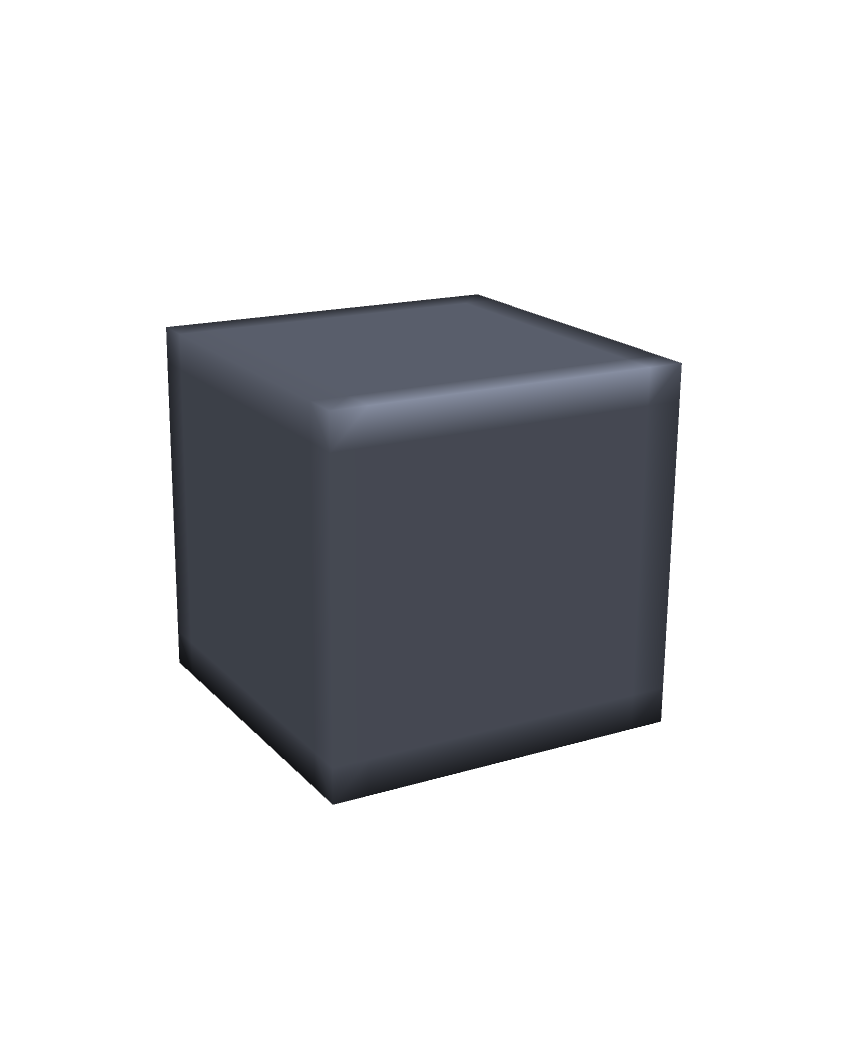
\includegraphics[width=0.24\textwidth]{resources/hexcli_00.png}
        \hfill
        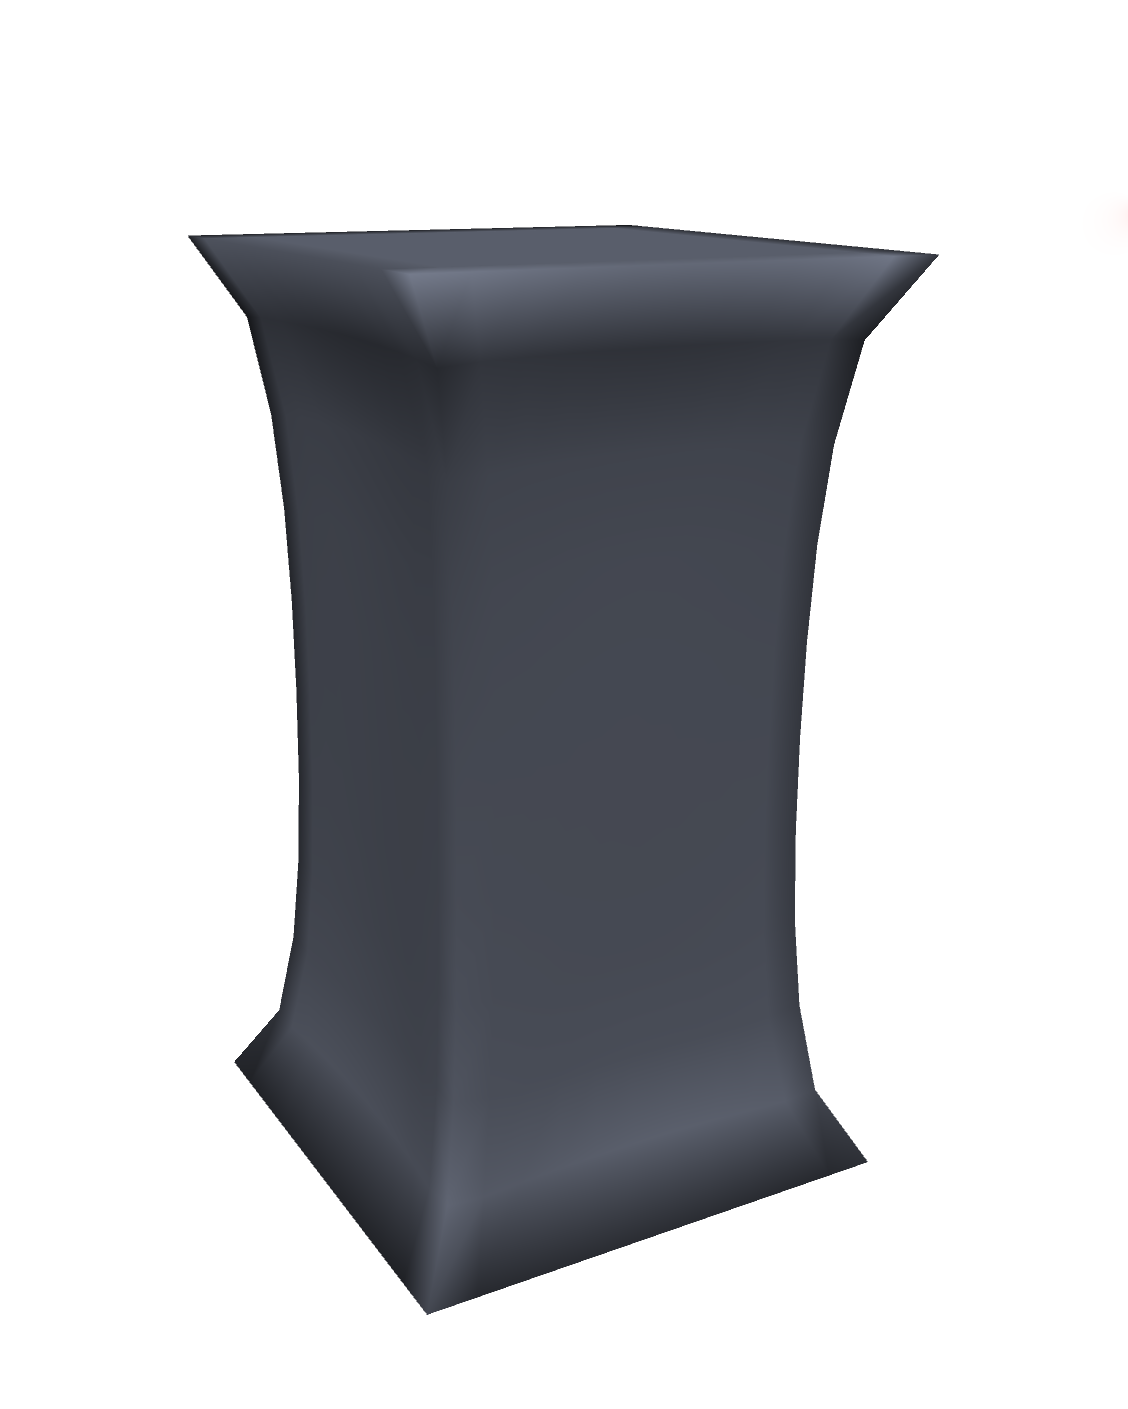
\includegraphics[width=0.24\textwidth]{resources/hexcli_08.png}
        \hfill
        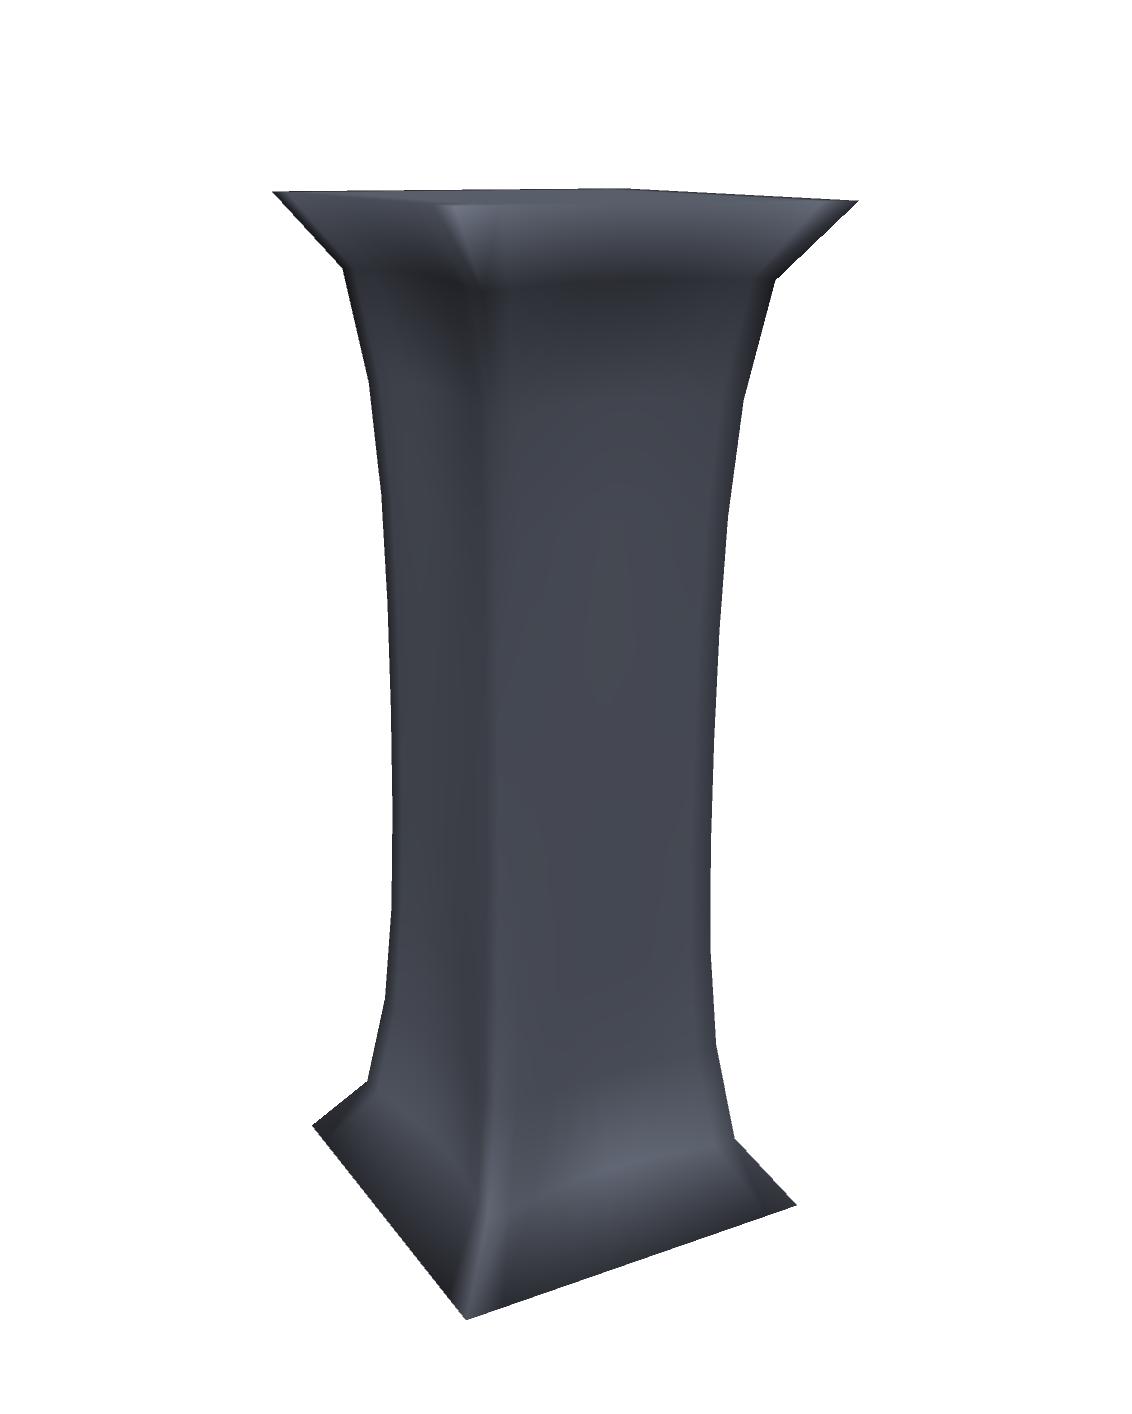
\includegraphics[width=0.24\textwidth]{resources/hexcli_16.png}
        \hfill
        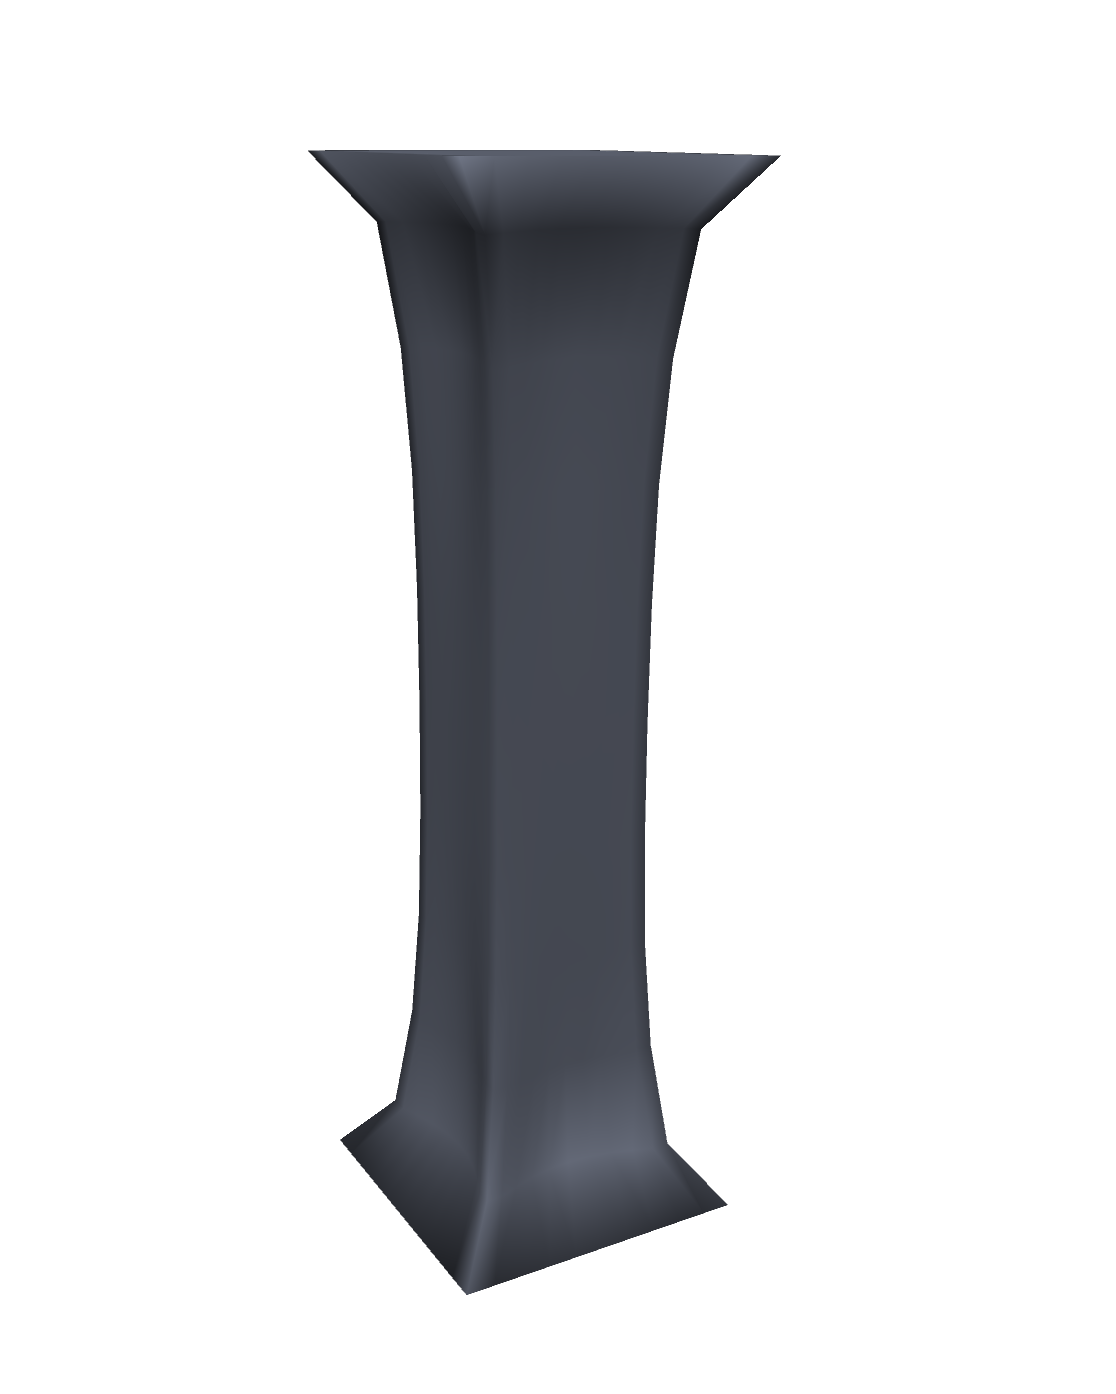
\includegraphics[width=0.24\textwidth]{resources/hexcli_24.png}
        \caption{Stretch test on a hexahedral mesh}
    \end{subfigure}
    \vskip\baselineskip
    \begin{subfigure}[b]{\textwidth}
        \centering
        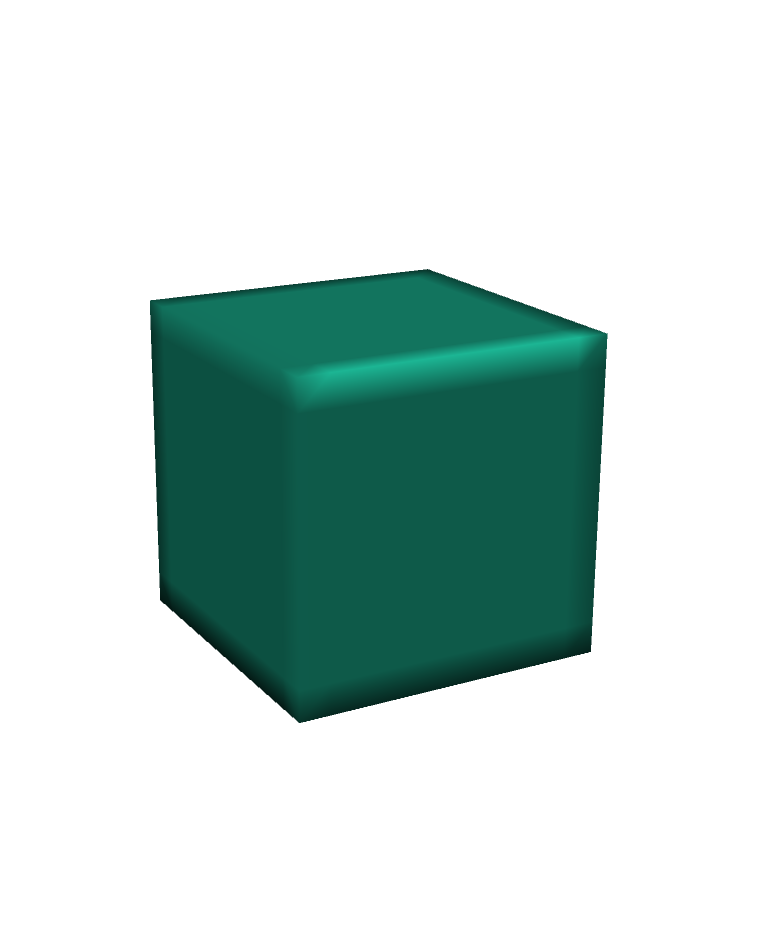
\includegraphics[width=0.24\textwidth]{resources/tetcli_00.png}
        \hfill
        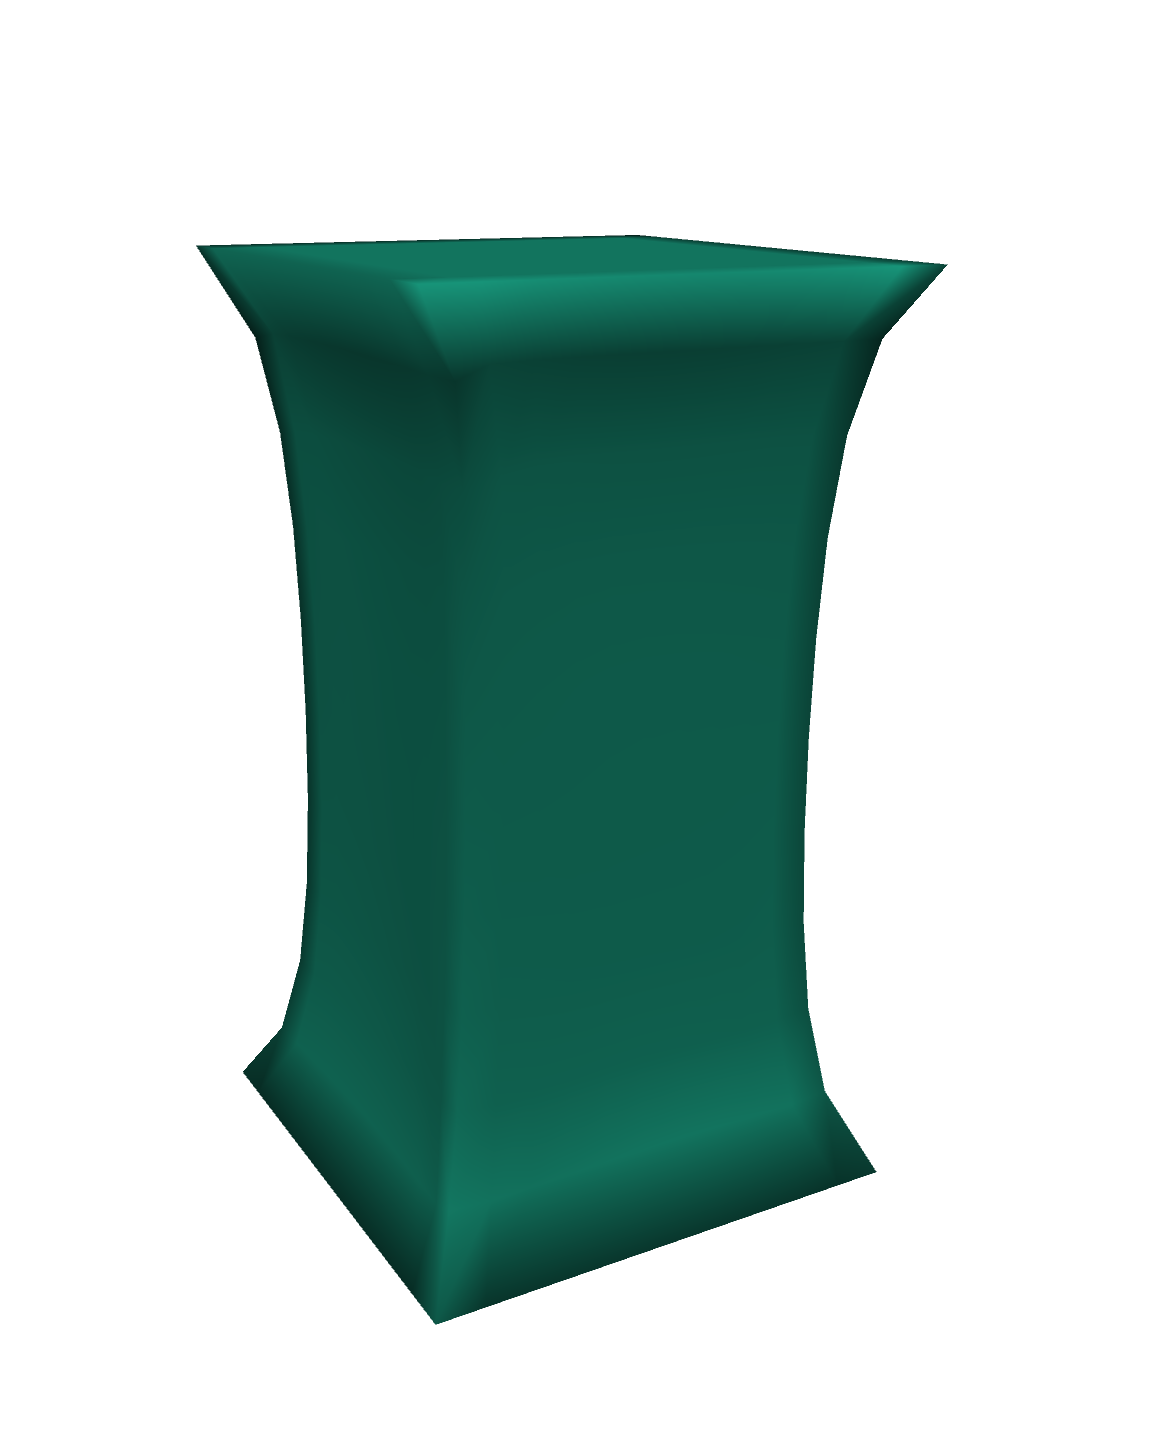
\includegraphics[width=0.24\textwidth]{resources/tetcli_08.png}
        \hfill
        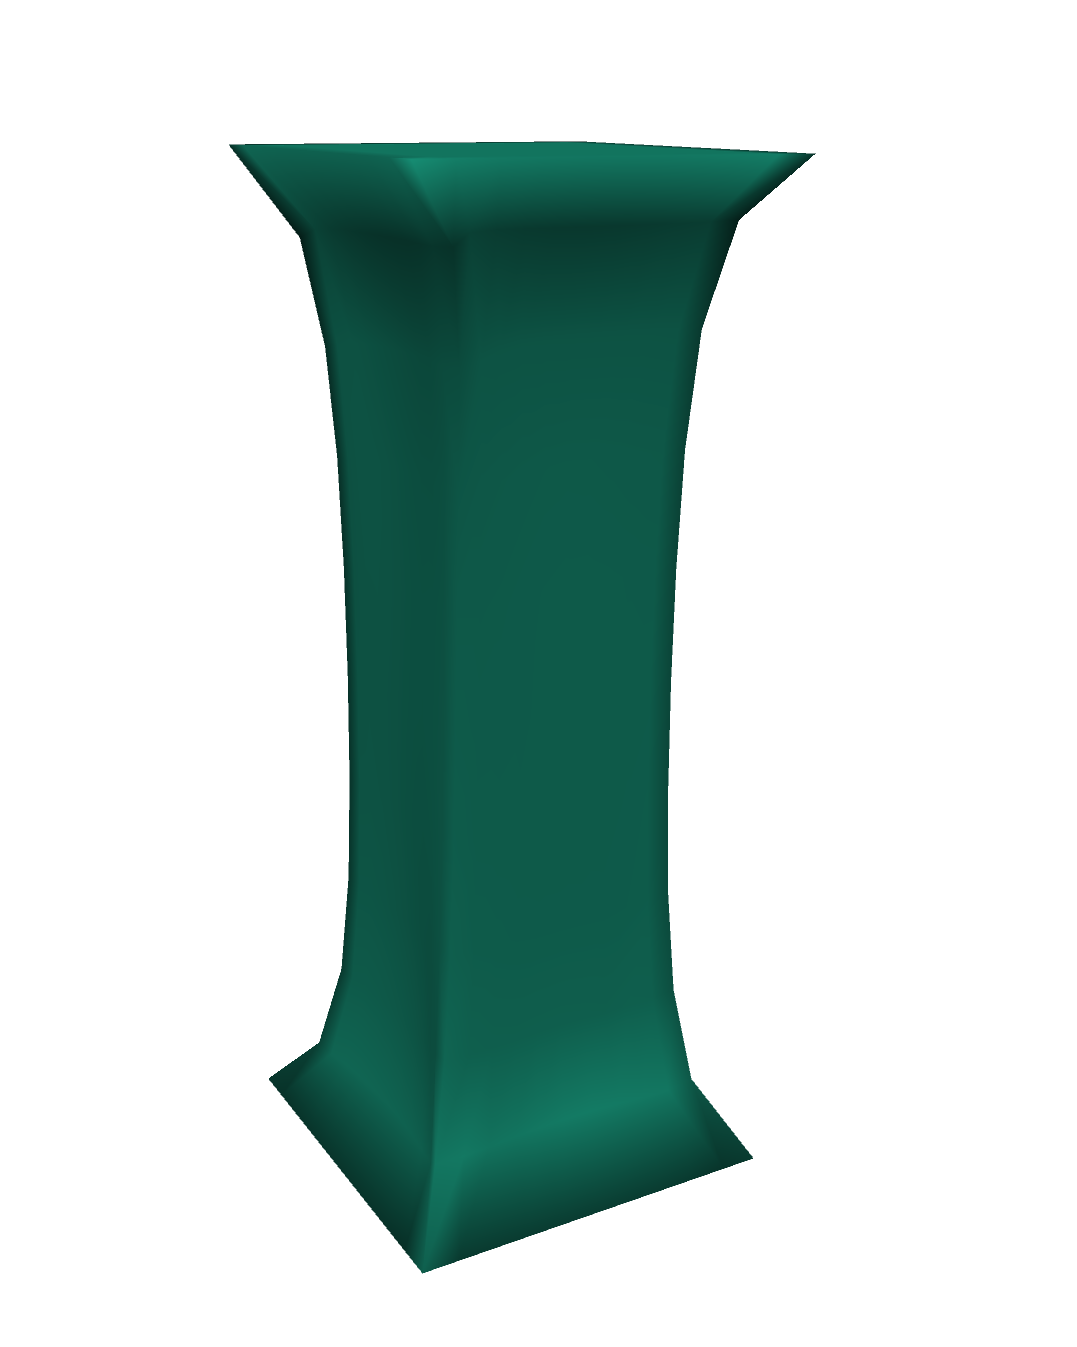
\includegraphics[width=0.24\textwidth]{resources/tetcli_16.png}
        \hfill
        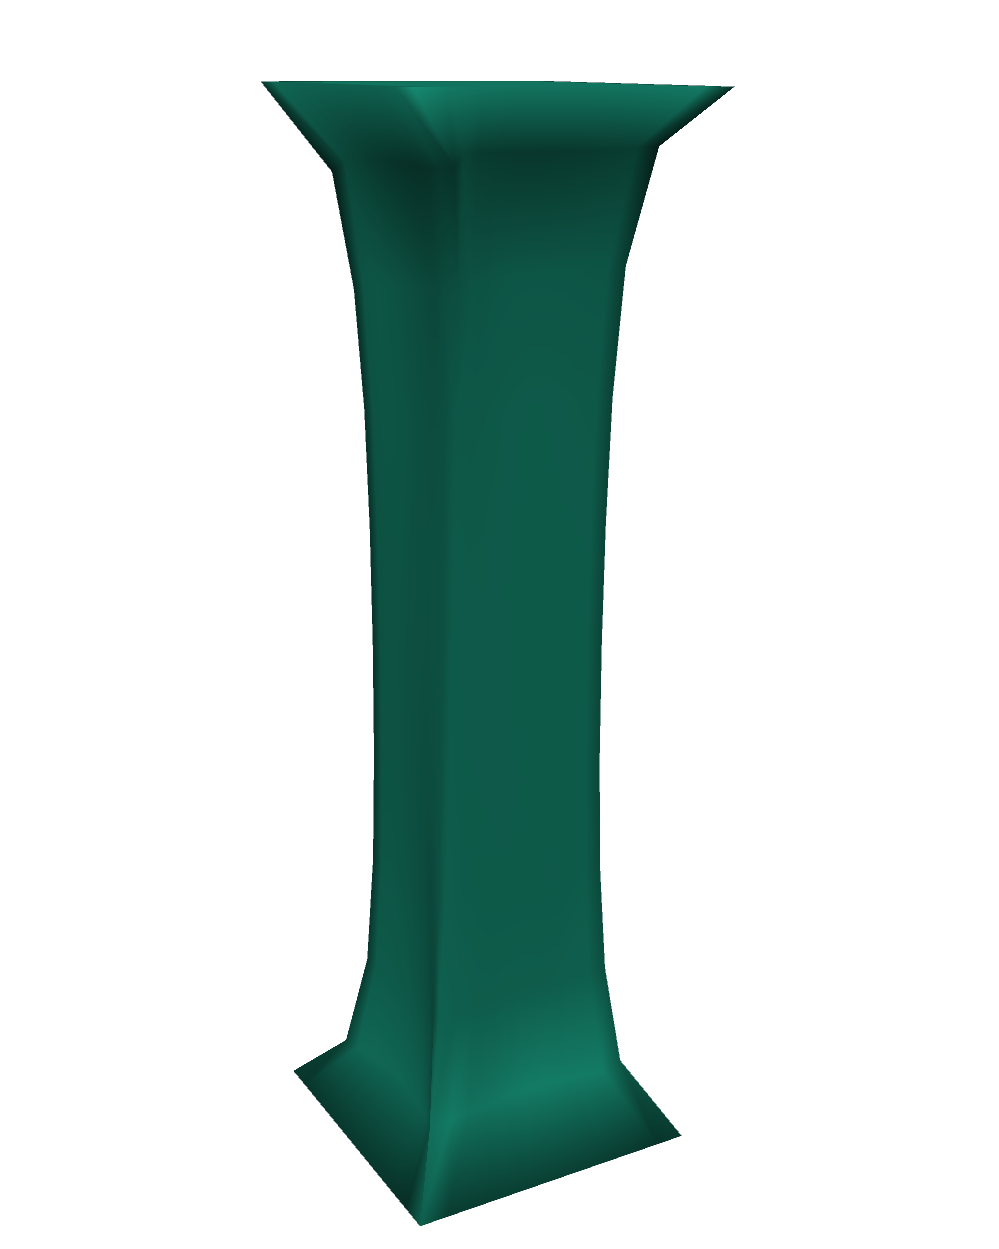
\includegraphics[width=0.24\textwidth]{resources/tetcli_24.png}
        \caption{Stretch test on a tetrahedral mesh}
    \end{subfigure}
    \caption[Stretch test performed on a cube]{Stretch test performed on a cube with (a) a hexahedral mesh and (b) a tetrahedral mesh with the same parameters}
    \label{fig:stretchtest}
\end{figure}

\subsection{Comparison of different Input Variables}
\label{ss:comparison_diff_vars}
In order to examine the influence of the input variables, I experimented with different values. The importance of the resolution is straight forward: With a higher resolution, the cube consists of more vertices and hexahedra or tetrahedra. In conclusion, the results are smoother, but we also increase the computational costs. 
For this example, I choose a resolution of 30 and let the other variables stay the same as in the previous example, meaning $\lambda = 10.0$ and $\mu = 1.0$, in order to make a comparison possible. If we choose a resolution of $30$, the cube consists of $29'791$ vertices and $162'000$ tetrahedra, respectively $27'000$ hexahedra. Thus, the cube consists of 27 times more cells than in the previous example.

Tables \ref{table:res_tet} and \ref{table:res_hex} show the amount of Newton iterations until a solution is reached. If we compare the numbers from this example with the ones from Table \ref{table:default_tet} and \ref{table:default_hex}, we can see that there are slightly more iterations needed than in the previous example. This increase can be expected due to the larger number of vertices and cells that the solver needs to consider.

\begin{table}[!htbp]
\parbox{.45\linewidth}{
\centering
\begin{tabular}{ | l | l |}
\hline
\textbf{Step number} & \textbf{Iterations} \\ \hline
1-7 & 3 \\ \hline
8-13 & 4 \\ \hline
14-20 & 5 \\ \hline
21-25 & 6 \\ \hline
\end{tabular}
\caption{Newton iterations for a tetrahedral mesh (res=30)}
\label{table:res_tet}
}
\hfill
\parbox{.45\linewidth}{
\centering
\begin{tabular}{ | l | l |}
\hline
\textbf{Step number} & \textbf{Iterations} \\ \hline
1-4 & 4 \\ \hline
5-10 & 5 \\ \hline
11-15 & 6 \\ \hline
16-19 & 7 \\ \hline
20-23 & 8 \\ \hline
24-25 & 9 \\ \hline
\end{tabular}
\caption{Newton iterations for a hexahedral mesh (res=30)}
\label{table:res_hex}
}
\end{table}

Fig. \ref{fig:res} shows the results with a higher resolution of $30$ compared to the lower resolution of $10$ of the previous example on a tetrahedral mesh. It shows the results of the deformation step $25$. We can see that a higher resolution clearly gives us more realistic results. Analogous, the same conclusion applies to the hexahedral mesh.
\begin{figure}[!ht]
\centering
\begin{subfigure}{.47\textwidth}
  \centering
  % include first image
  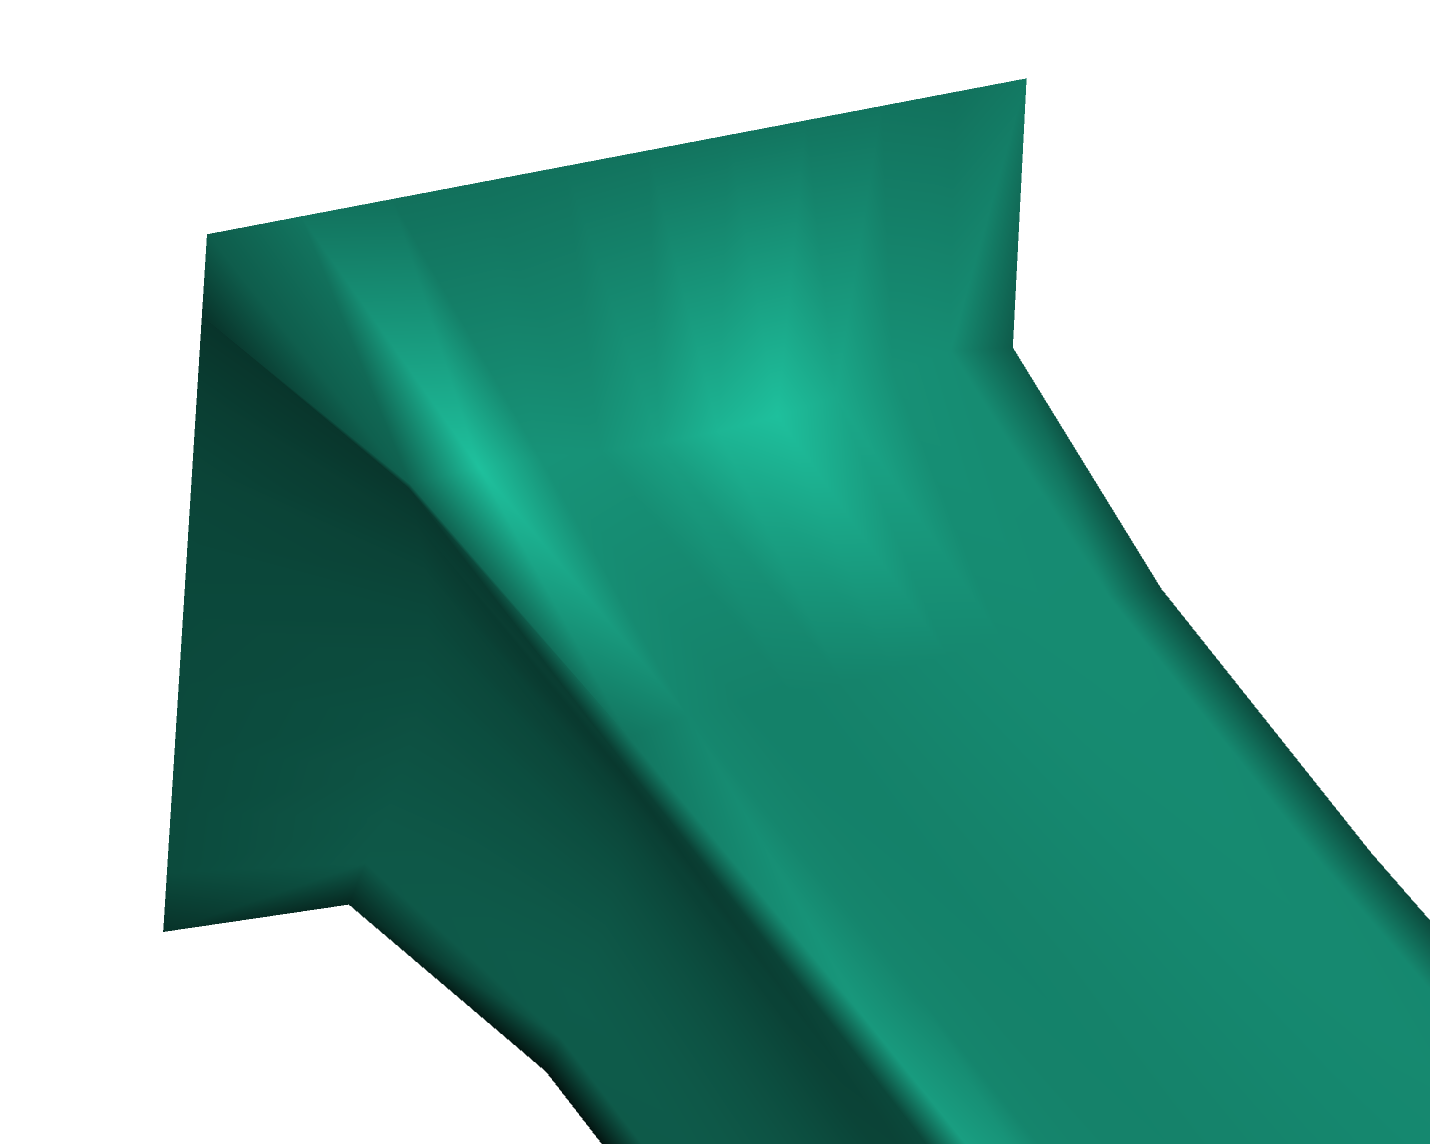
\includegraphics[width=.8\linewidth]{resources/default_zoom_tet.png}  
  \caption{Step 25 with a resolution of 10}
  \label{fig:res_1}
\end{subfigure}
\begin{subfigure}{.47\textwidth}
  \centering
  % include second image
  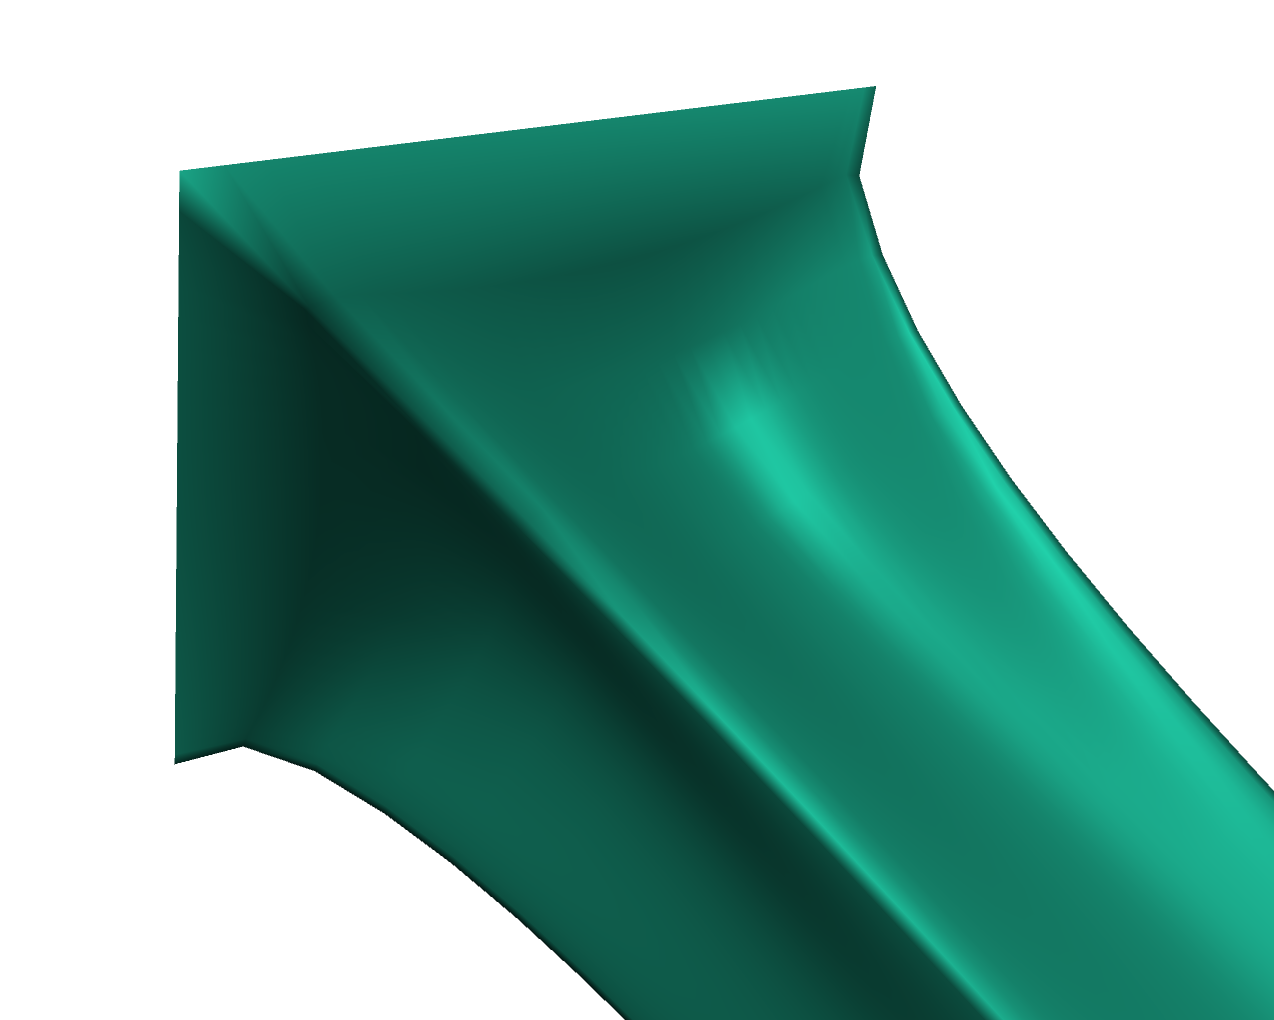
\includegraphics[width=.8\linewidth]{resources/res_zoom_tet.png}  
  \caption{Step 25 with a resolution of 30}
  \label{fig:res_2}
\end{subfigure}
\caption{Results with a different resolution on a tetrahedral mesh}
\label{fig:res}
\end{figure}

In addition, we can increase or decrease the Lamé parameters \textit{\mu} and \textit{\lambda}, which influences the Poisson's ratio directly. If we decrease \textit{\lambda}, the Poisson's ratio also decreases. We can set \textit{\lambda} equal to $1.0$ and let the other variables stay the same as in the previous example. Thus, $\mu$ is equal to 1.0, and the resolution is set to 30.0. The Poisson's ratio indicates the extent of the deformation. Materials with a higher value are more easily deformable, which I explained in \autoref{ss:material_constants}. Therefore, by decreasing the Poisson's ratio, the extent of the deformation is also decreased. That affects the resulting object as well as the computational costs. Tables \ref{table:lambda_tet} and \ref{table:lambda_hex} show the amount of Newton iteration needed for the chosen input values. The amount of iterations has decreased for both meshes. We need fewer iterations because the extent of the deformation is smaller than before.

\begin{table}[!htbp]
\parbox{.45\linewidth}{
\centering
\begin{tabular}{ | l | l |}
\hline
\textbf{Step number} & \textbf{Iterations} \\ \hline
1-25 & 3 \\ \hline
\end{tabular}
\caption{Newton iterations for a tetrahedral mesh ($\lambda = 1.0$)}
\label{table:lambda_tet}
}
\hfill
\parbox{.45\linewidth}{
\centering
\begin{tabular}{ | l | l |}
\hline
\textbf{Step number} & \textbf{Iterations} \\ \hline
1-25 & 4 \\ \hline
\end{tabular}
\caption{Newton iterations for a hexahedral mesh ($\lambda = 1.0$)}
\label{table:lambda_hex}
}
\end{table}

Fig. \ref{fig:lambda} shows how the deformation is influenced by changing $\lambda$. With these inputs, the cube gets wider in the middle part, as a lower Poisson's ratio indicates that the material is more resistant to stretching.
\begin{figure}[!ht]
\centering
\begin{subfigure}{.47\textwidth}
  \centering
  % include first image
  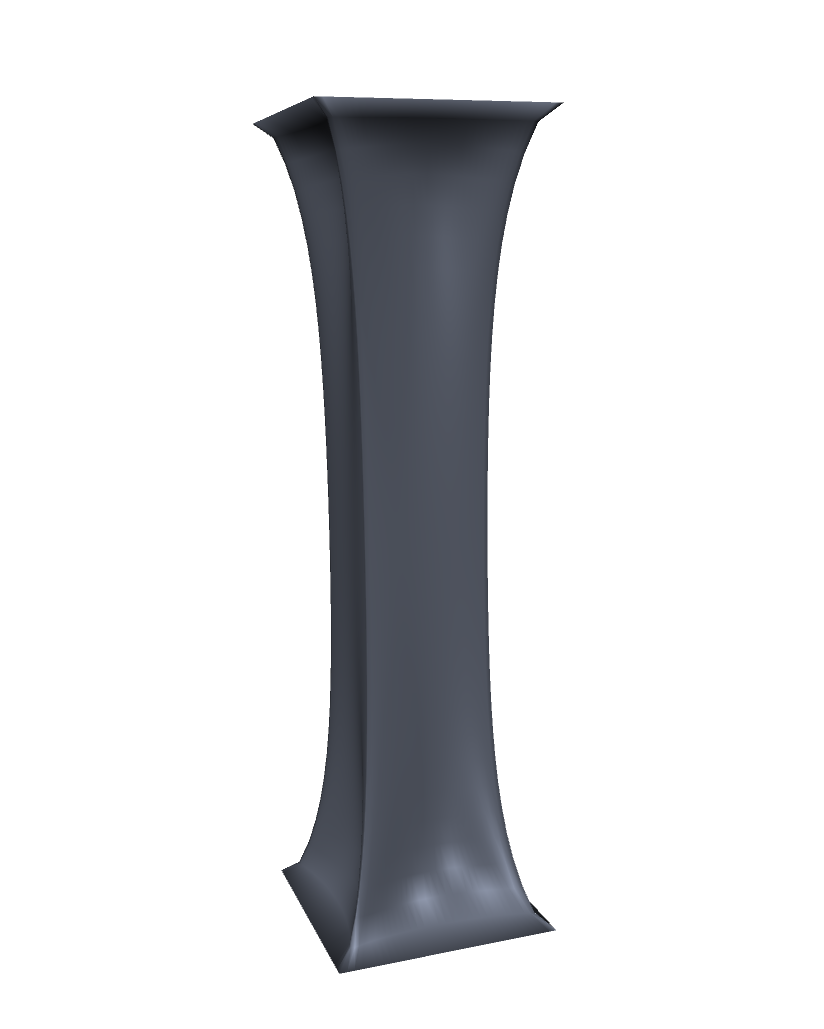
\includegraphics[width=.75\linewidth]{resources/lambda_comparison_res.png}  
  \caption{Step 25 with $\lambda = 10.0$}
  \label{fig:lambda_1}
\end{subfigure}
\begin{subfigure}{.47\textwidth}
  \centering
  % include second image
  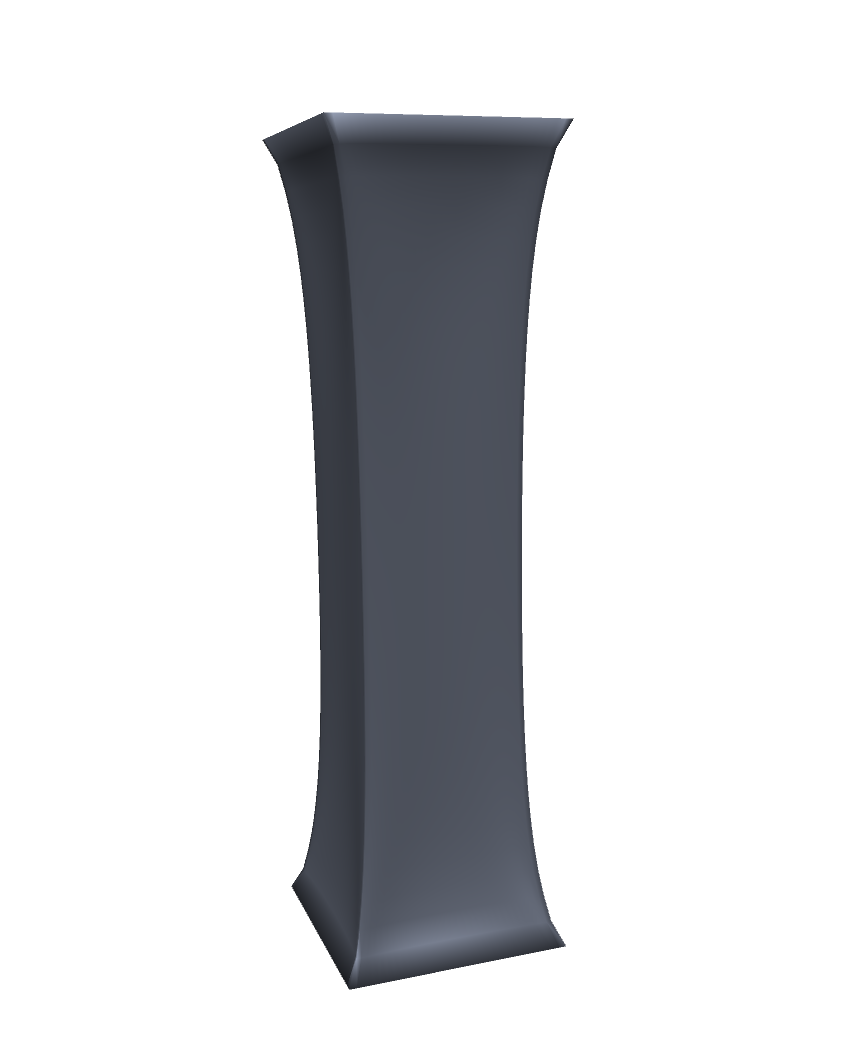
\includegraphics[width=.75\linewidth]{resources/lambda_comparison_lambda.png}  
  \caption{Step 25 with $\lambda = 1.0$}
  \label{fig:lambda_2}
\end{subfigure}
\caption{Results with different values for $\lambda$ on a hexahedral mesh}
\label{fig:lambda}
\end{figure}

Now instead of decreasing the Poisson's ratio, let's increase it. We can achieve that by choosing $\mu = 0.1$ and set $\lambda$ equal to 10.0 and let the resolution be 30. This is an extreme case because the Poisson's ratio is very close to $0.5$. It is also an appropriate value for simulating flesh behaviour. Tables \ref{table:mu_tet} and \ref{table:mu_hex} illustrate the amount of Newton iterations needed for this configuration. As we can see, we need more Newton iterations to solve the system. That is caused by the increased deformation, as the cube gets narrower in the middle part, which makes reaching a good solution more difficult.

\begin{table}[!htbp]
\parbox{.45\linewidth}{
\centering
\begin{tabular}{ | l | l |}
\hline
\textbf{Step number} & \textbf{Iterations} \\ \hline
1 & 3 \\ \hline
2-3 & 4 \\ \hline
4-6 & 5 \\ \hline
7 & 6 \\ \hline
8-11 & 7 \\ \hline
12 & 8 \\ \hline
13-20 & 9 \\ \hline
21-25 & 11 \\ \hline
\end{tabular}
\caption{Newton iterations for a tetrahedral mesh ($\mu = 0.1$)}
\label{table:mu_tet}
}
\hfill
\parbox{.45\linewidth}{
\centering
\begin{tabular}{ | l | l |}
\hline
\textbf{Step number} & \textbf{Iterations} \\ \hline
1 & 6 \\ \hline
2 & 7 \\ \hline
3 & 8 \\ \hline
4 & 9 \\ \hline
5-6 & 10 \\ \hline
7 & 11 \\ \hline
8-9 & 12 \\ \hline
10-11 & 13 \\ \hline
12 & 14 \\ \hline
13-14 & 15 \\ \hline
15 & 16 \\ \hline
16 & 17 \\ \hline
17-19 & 18 \\ \hline
20-25 & 20 \\ \hline
\end{tabular}
\caption{Newton iterations for a hexahedral mesh ($\mu = 0.1$)}
\label{table:mu_hex}
}
\end{table}

A higher Poisson's value makes the cube more susceptible to stretching. We can see this effect a bit by comparing the two images in Fig. \ref{fig:mu}, although the difference is not extreme because the Poisson's ratios for the two examples are close to each other. The first image shows a material with a Poisson's ratio of approximately 0.46, and the second image shows a material with a Poisson's ratio approaching 0.5. The model behaves well with these input values, and no artefacts can be seen.
\begin{figure}[!ht]
\centering
\begin{subfigure}{.47\textwidth}
  \centering
  % include first image
  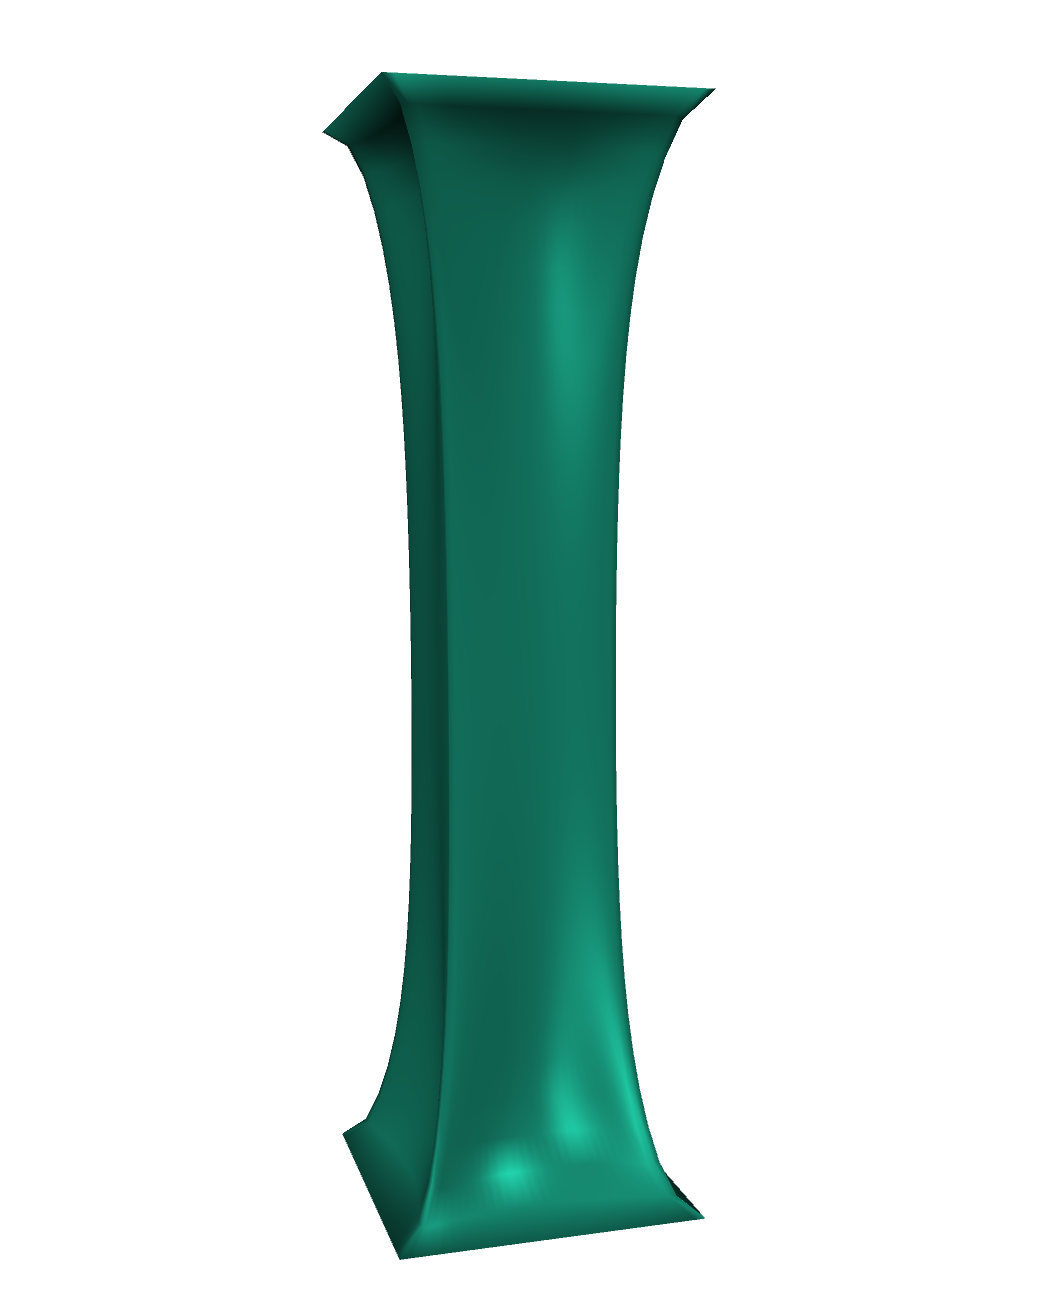
\includegraphics[width=.75\linewidth]{resources/mu_res_new.png}  
  \caption{Step 25 with $\mu = 1.0$}
  \label{fig:mu_1}
\end{subfigure}
\begin{subfigure}{.47\textwidth}
  \centering
  % include second image
  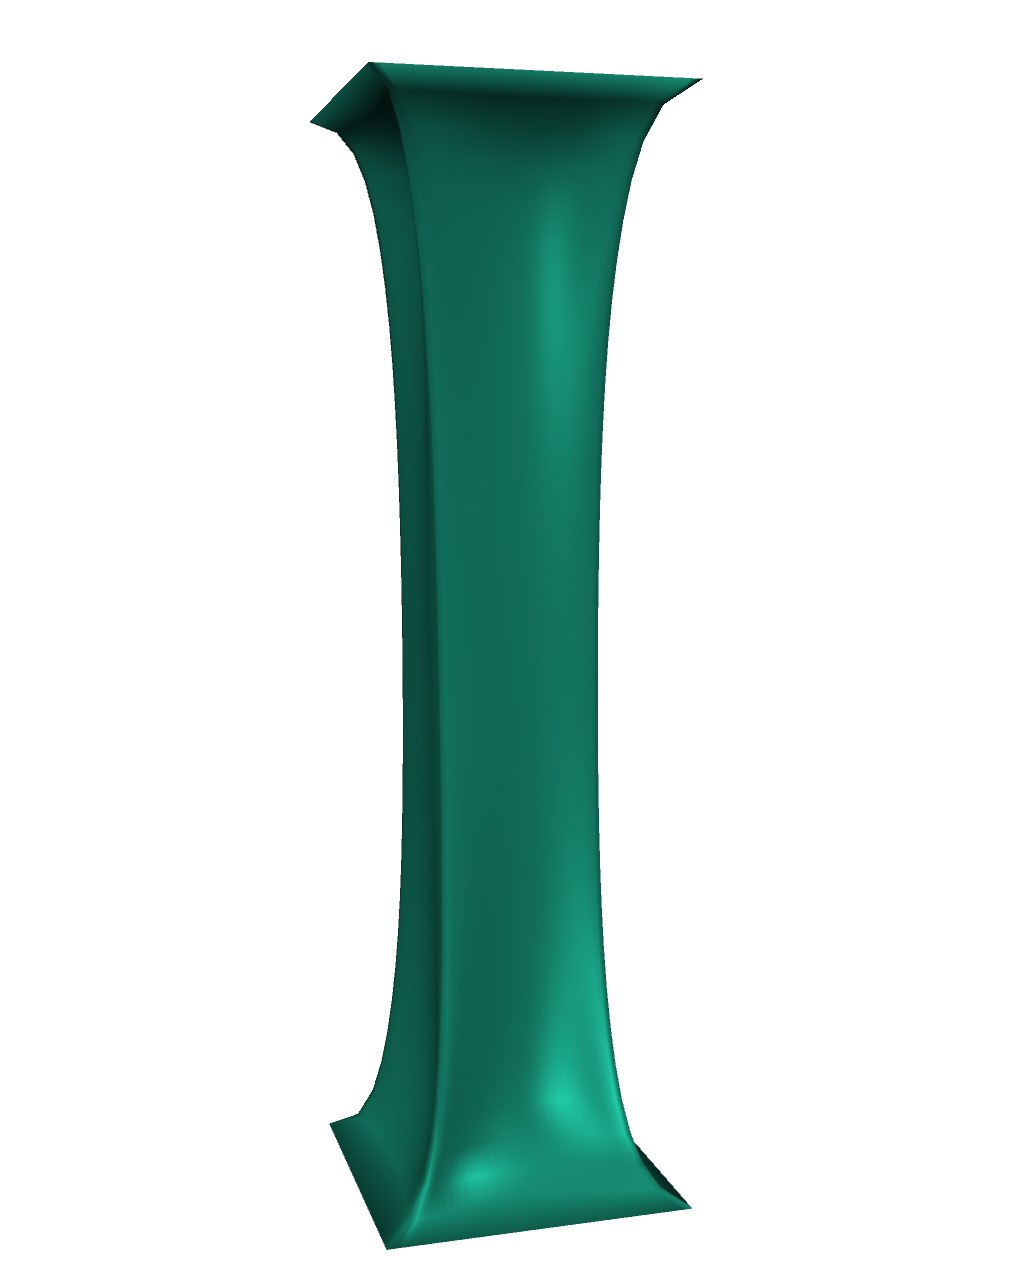
\includegraphics[width=.75\linewidth]{resources/mu_mu_new.png}  
  \caption{Step 25 with $\mu = 0.1$}
  \label{fig:mu_2}
\end{subfigure}
\caption{Results with different values for $\mu$ on a tetrahedral mesh}
\label{fig:mu}
\end{figure}

\newpage
\section{Additional Tests}
\label{s:generalization}
For this section, I changed some parts of the given implementation to perform more tests for this new energy. The first thing I did was to change the code, such that I was able to perform a quasi-static simulation of the stretching of an arbitrary mesh. Similar to the provided code, there are again 25 deformation steps. The implementation expects as input a tetrahedral or hexahedral mesh in the format .ovm (OpenVolumeMesh). In the user interface, several values can be selected:
\begin{itemize}
	\item Mesh type: Describes the cell shape of the mesh. The cell shape can be either \textit{tetrahedral}, \textit{regular hexahedral}, or \textit{irregular hexahedral}.
	\item Lambda: One of the Lamé parameters that determine the Poisson's ratio.
	\item Mu: One of the Lamé parameters that determine the Poisson's ratio.
	\item Stretch axis: Axis along which the mesh is supposed to be stretched. This can be the \textit{x}-, \textit{y}-, or \textit{z}-axis.
	\item Coordinate value for the first boundary: Determines the position at which the first boundary face lies.
	\item Coordinate value for the second boundary: Determines the position at which the second boundary face lies.
	\item Rate of step size: Rate at which the object should be stretched along the axis.
\end{itemize}

The rate of step size corresponds to the variable \verb|stepDelta| in \autoref{lst:newBoundary}. I made this variable adjustable because we are dealing with arbitrary meshes that could potentially be very large or very small. For better results, we might want to change the rate at which we stretch the object. 

In order to get the desired results, I had to adjust the code accordingly. Fig. \ref{fig:procedure_generalization} illustrates the modified procedure of the code. The green fields are the steps that are different from the procedure before. Although the writing of the file was necessary before, it is explicitly listed here because the output format of the file has changed. In addition, the general procedure of updating the boundary conditions also stayed the same, but I had to adjust some parts so that the user input is processed correctly.

\begin{figure}[!htb]
\centering
\begin{tikzpicture}[node distance=2cm]
\node (input) [process] {$\mu$, $\lambda$, resolution};
\node (code1) [decision, right of=input, xshift=1.9cm] {Initialize material model};
\node (code6) [io, right of=code1, xshift=1cm] {Write file};
\node (code2) [io, below of=code1, yshift=-0.5cm] {Load mesh};
\node (code3) [io, below of=code2, yshift=-0.5cm] {Convert mesh};
\node (code4) [io, right of=code3, xshift=1cm] {Update boundary conditions};
\node (code5) [decision, below of=code6, yshift=-0.5cm] {Newton solve};
\node (output) [process, right of=code6, xshift=1.9cm] {26 objects};

\draw [arrow] (input) -- node[anchor=south] {Input}(code1);
\draw [arrow] (code1) -- (code2);
\draw [arrow] (code2) -- (code3);
\draw [arrow] (code3) -- (code4);
\draw [arrow] (code4) -- (code5);
\draw [arrow] (code5) -- (code6);
\draw [arrow] (code6) -- node[anchor=south] {Output}(output);
\end{tikzpicture}
\caption{Illustration of the modified procedure} \label{fig:procedure_generalization}
\end{figure}

The initialization of the material model stays the same as before. But now the implementation needs to load the mesh the user provides into the system. It then converts the input mesh into the data structure that was used by the provided code. Additionally, if the user input states that a hexahedral mesh is irregular, each hexahedron gets subdivided into four tetrahedra. This step was necessary because the subsequent steps expect the hexahedral mesh to be regular. Then, the boundary conditions are updated according to the input of the user. The stretching is again done by putting the boundary faces further away from each other along the stretch axis. Afterwards, the Newton solver calculates the final position of each vertex that is not fixed. Finally, the mesh is written into a file of the format .ovm (OpenVolumeMesh).

\subsection{Cylinder}
With the adjusted code, I was able to recreate the example of stretching a cylinder. This example was shown in the paper \acrshort{snh}, and the authors claimed that their model can handle this deformation well, even with a high Poisson's ratio and no parameter tuning. For my experiments, I used a hexahedral mesh consisting of $1'290$ vertices and $1'036$ hexahedra. Similar to the previous examples of the stretching of a cube, Fig. \ref{fig:stretchtest_cylinder} shows step 0 (initial cylinder), 8, 16, and 24 of the deformation. For the parameters, I chose $\lambda = 10.0$, $\mu = 1.0$, and a step size of 0.1, in order to reach a high Poisson's ratio and to get a large stretch of the object.
\begin{figure}[!htbp]
    \centering
    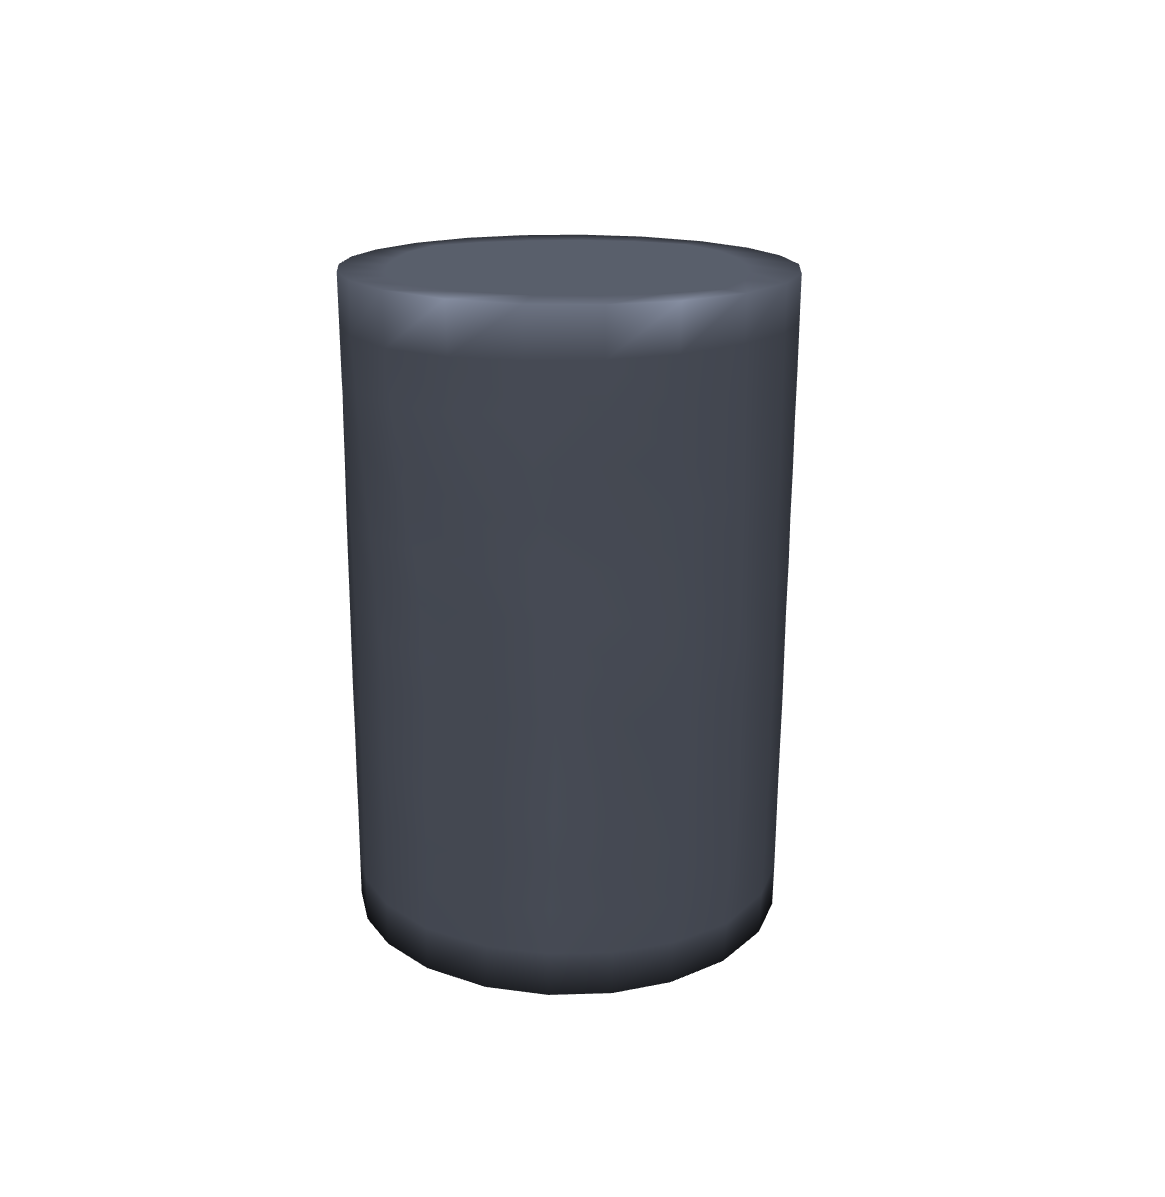
\includegraphics[width=0.24\textwidth]{resources/cylinder_00_new.png}
    \hfill
    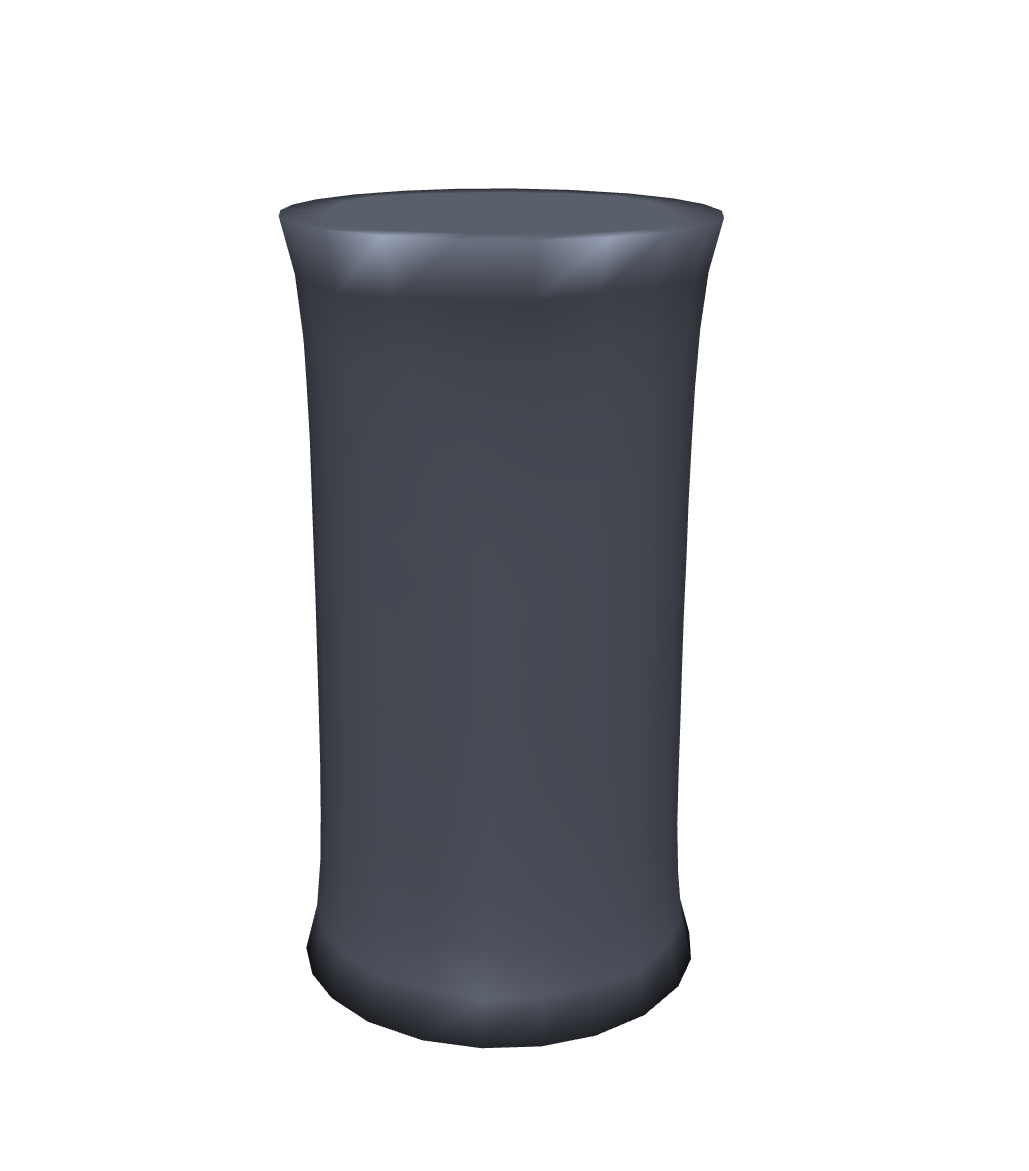
\includegraphics[width=0.24\textwidth]{resources/cylinder_08_new.png}
    \hfill
    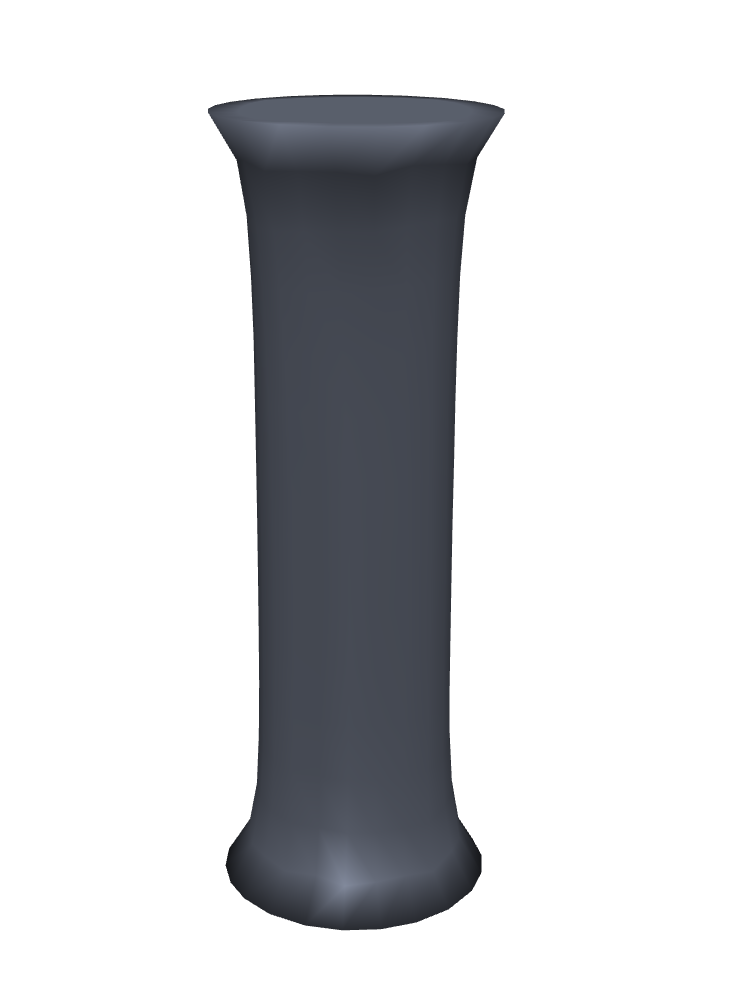
\includegraphics[width=0.24\textwidth]{resources/cylinder_16_new.png}
    \hfill
    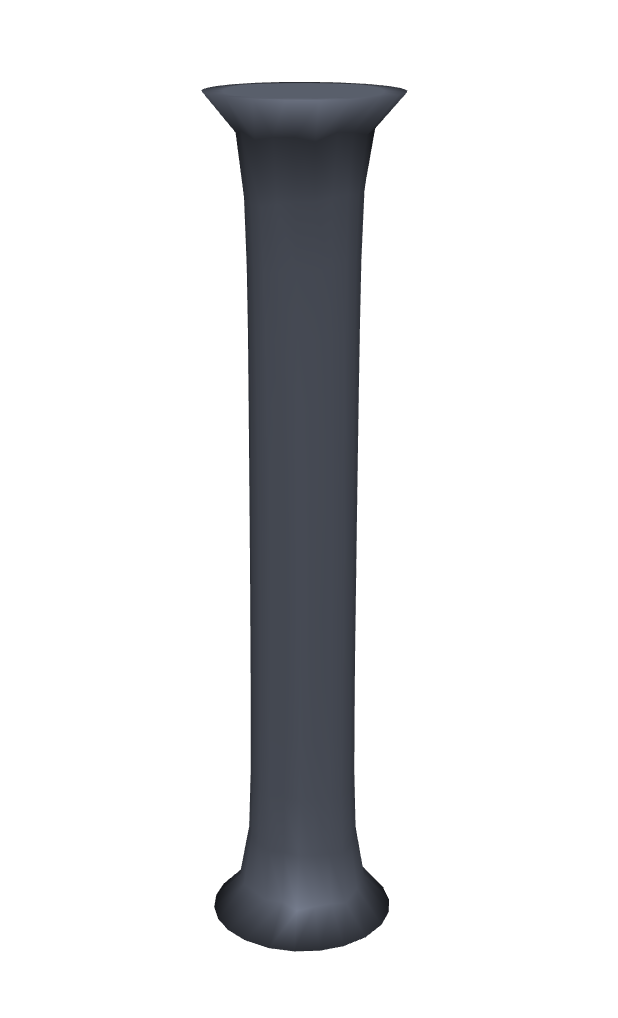
\includegraphics[width=0.24\textwidth]{resources/cylinder_24_new.png}
    \hfill
    \caption{Stretch test on a cylinder}
    \label{fig:stretchtest_cylinder}
\end{figure}

The images verify the claims of the authors. The deformation is captured well and no artifacts can be seen, even for a larger stretch. Therefore, we can assume that we are not restricted to a specific shape of the deformable object. In addition, Table \ref{table:cylinder} illustrates the amount of Newton iterations that were necessary for solving the system. The numbers are a bit higher for a larger stretch compared to the cube, which consists of a similar amount of hexahedra. But they are still in a reasonable interval. 

\begin{table}[!htbp]
\parbox{.45\linewidth}{
\centering
\begin{tabular}{ | l | l |}
\hline
\textbf{Step number} & \textbf{Iterations} \\ \hline
1 & 2 \\ \hline
2-7 & 3 \\ \hline
8-12 & 4 \\ \hline
13-14 & 5 \\ \hline
15-16 & 6 \\ \hline
17-18 & 7 \\ \hline
\end{tabular}
}
\hfill
\parbox{.45\linewidth}{
\centering
\begin{tabular}{ | l | l |}
\hline
\textbf{Step number} & \textbf{Iterations} \\ \hline
19-20 & 8 \\ \hline
21 & 9 \\ \hline
22 & 10 \\ \hline
23-24 & 11 \\ \hline
25 & 13 \\ \hline
\end{tabular}
}
\caption{Newton iterations for the deformation of a cylinder}
\label{table:cylinder}
\end{table}

\subsection{Scramble Test}
In order to highlight the robustness of the model, the authors performed a scramble test similar to those in Teran et al. (\cite{teran2005robust}) and Stomakin et al. (\cite{stomakhin2012energetically}). For this test, they randomly placed the vertices of a cube within a space of twice its rest volume. This test illustrates how the model performs under extreme, inverted configurations. Fig. \ref{fig:scramble} shows the results of the scramble test I performed.
\begin{figure}[!htbp]
	\centering
	\begin{subfigure}[b]{\textwidth}
        \centering
        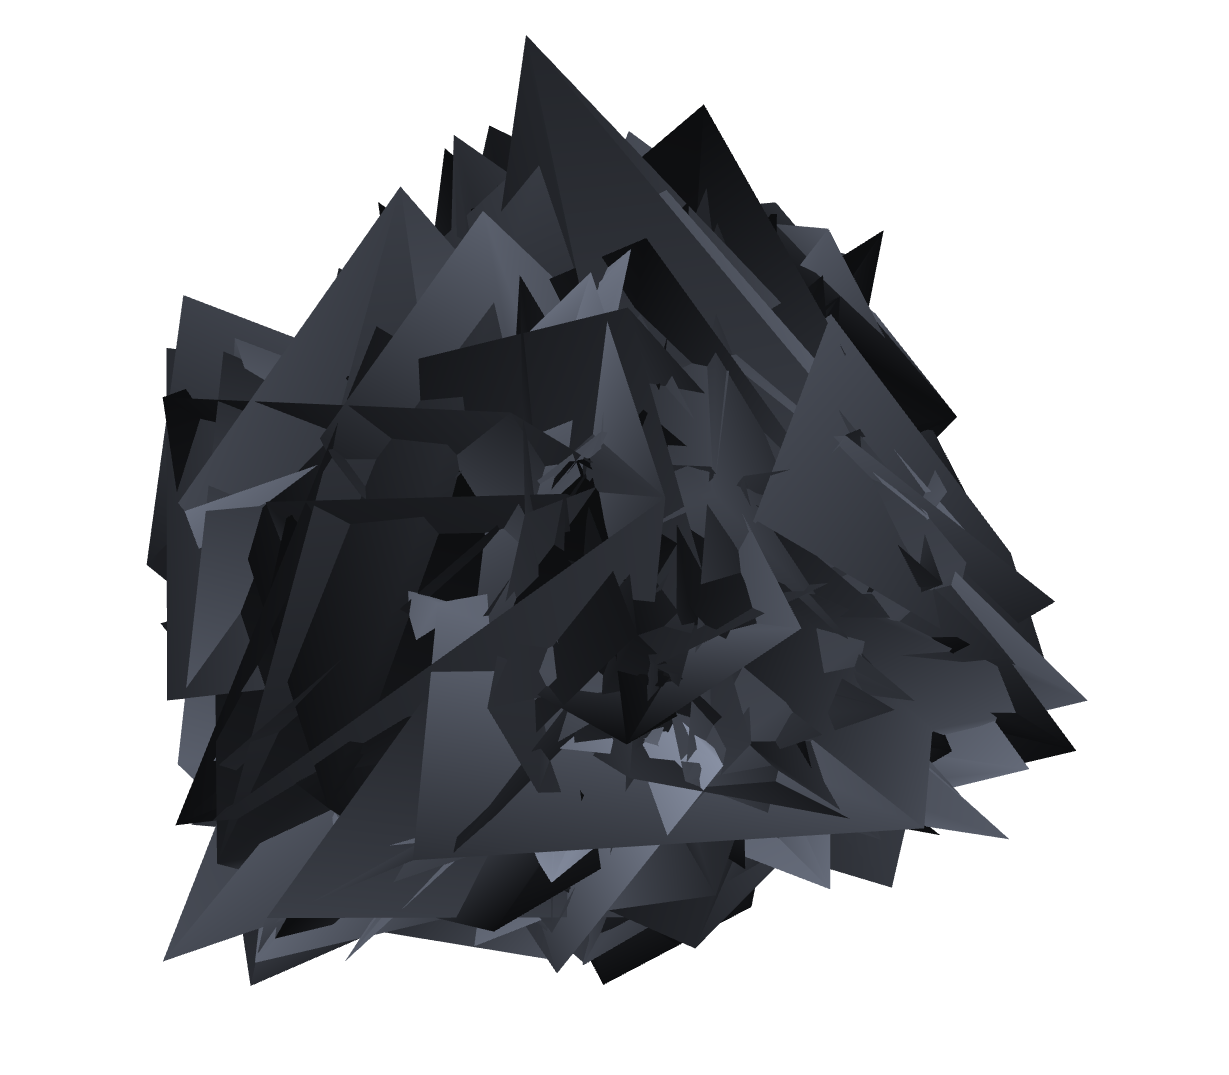
\includegraphics[width=0.32\textwidth]{resources/scramble_00_new.png}
        \hfill
        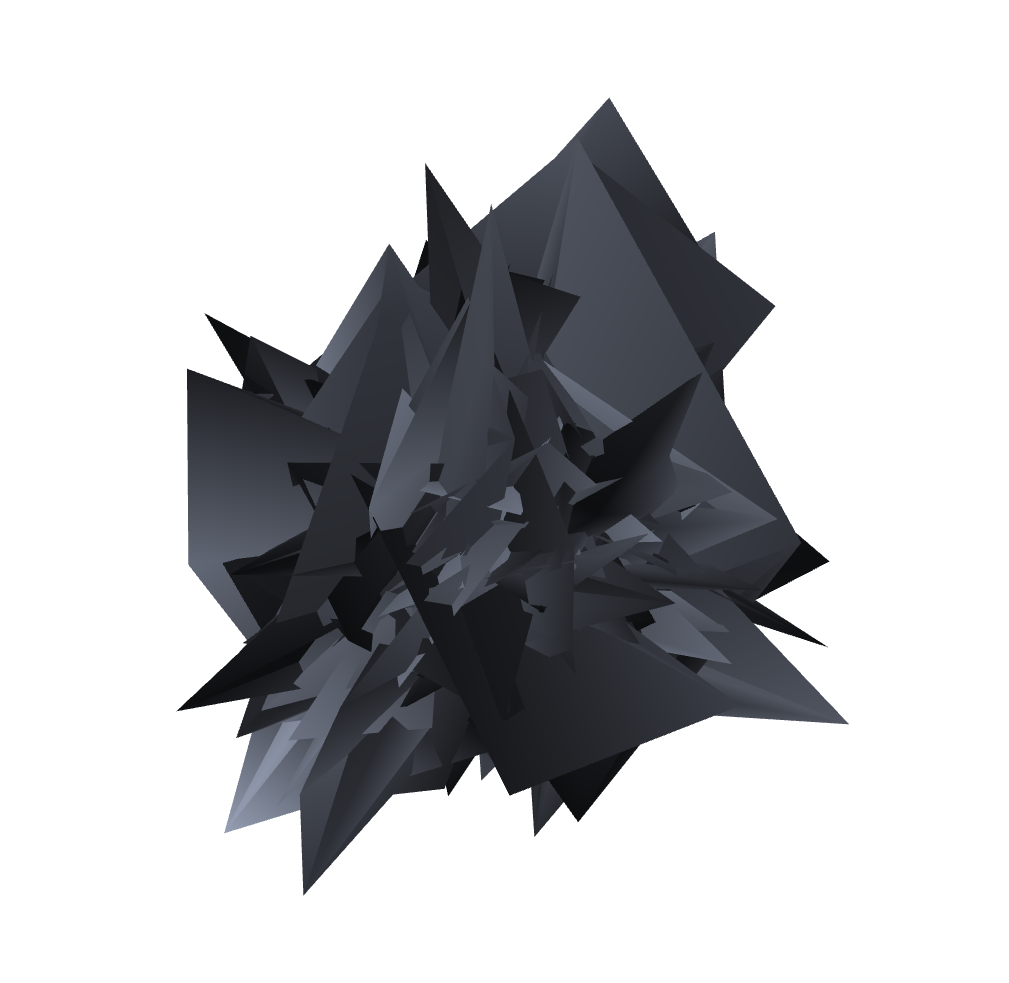
\includegraphics[width=0.32\textwidth]{resources/scramble_01_new.png}
        \hfill
        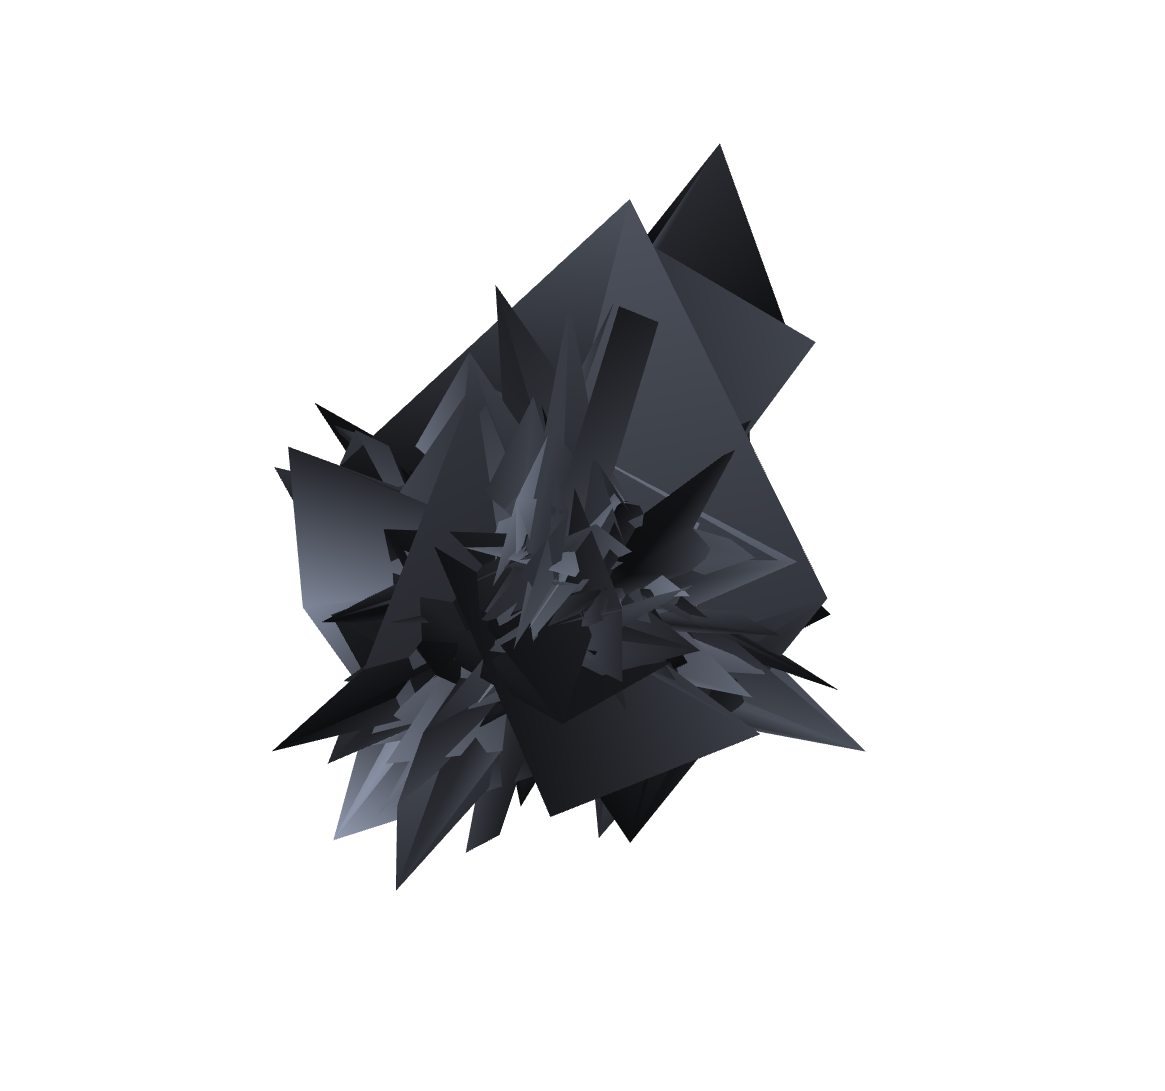
\includegraphics[width=0.32\textwidth]{resources/scramble_02_new.png}
        \caption{Results after 0, 1, and 2 Newton iterations (from left to right)}
    \end{subfigure}
    \vskip\baselineskip
    \begin{subfigure}[b]{\textwidth}
        \centering
        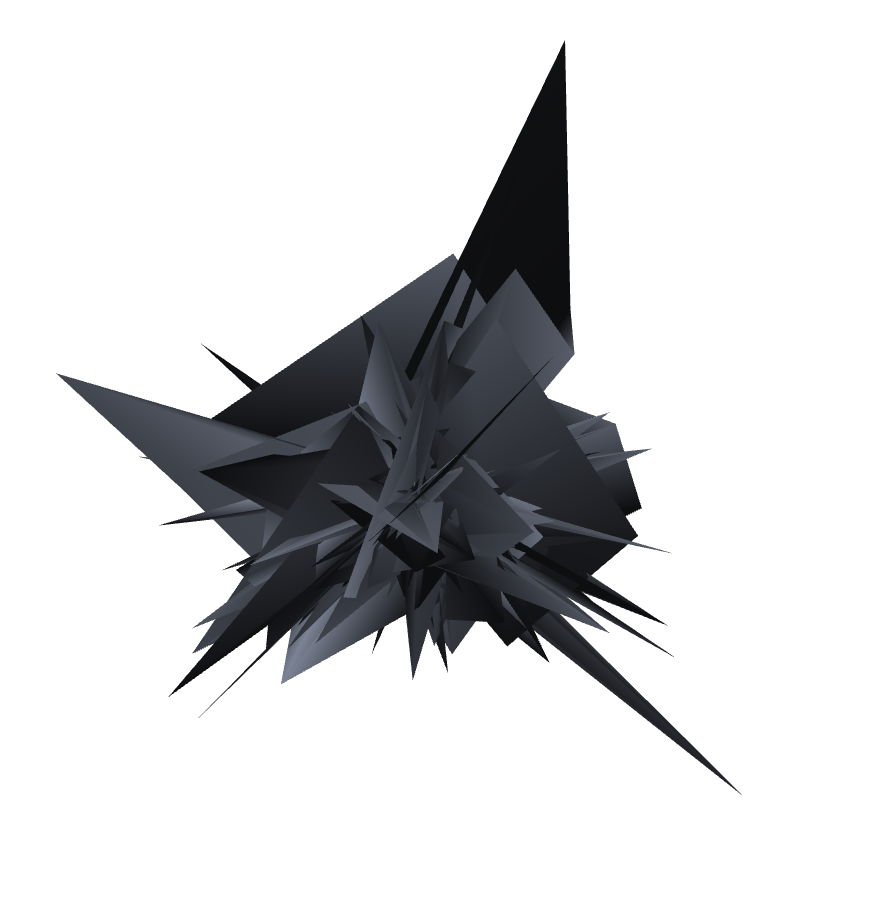
\includegraphics[width=0.32\textwidth]{resources/scramble_03_new.png}
        \hfill
        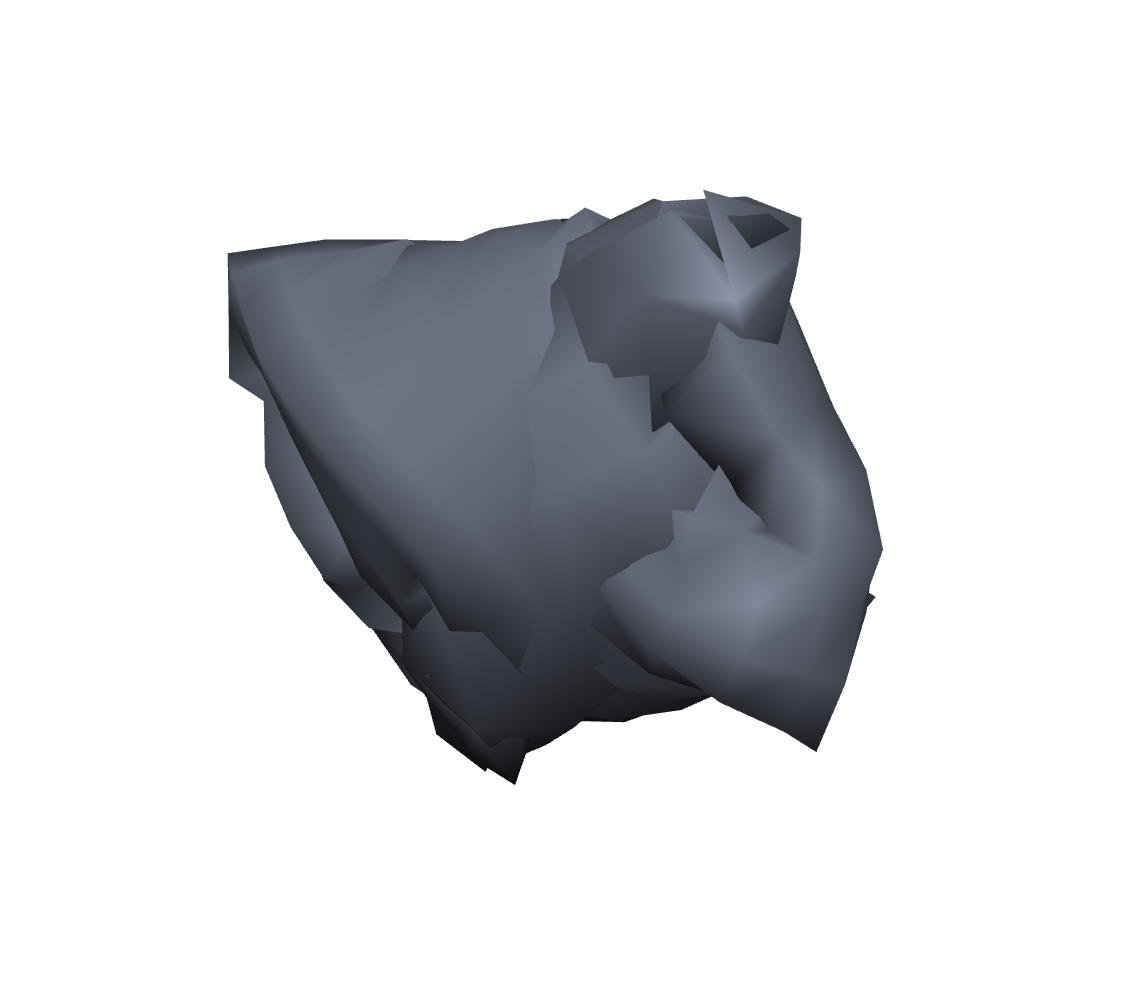
\includegraphics[width=0.32\textwidth]{resources/scramble_04_new.png}
        \hfill
        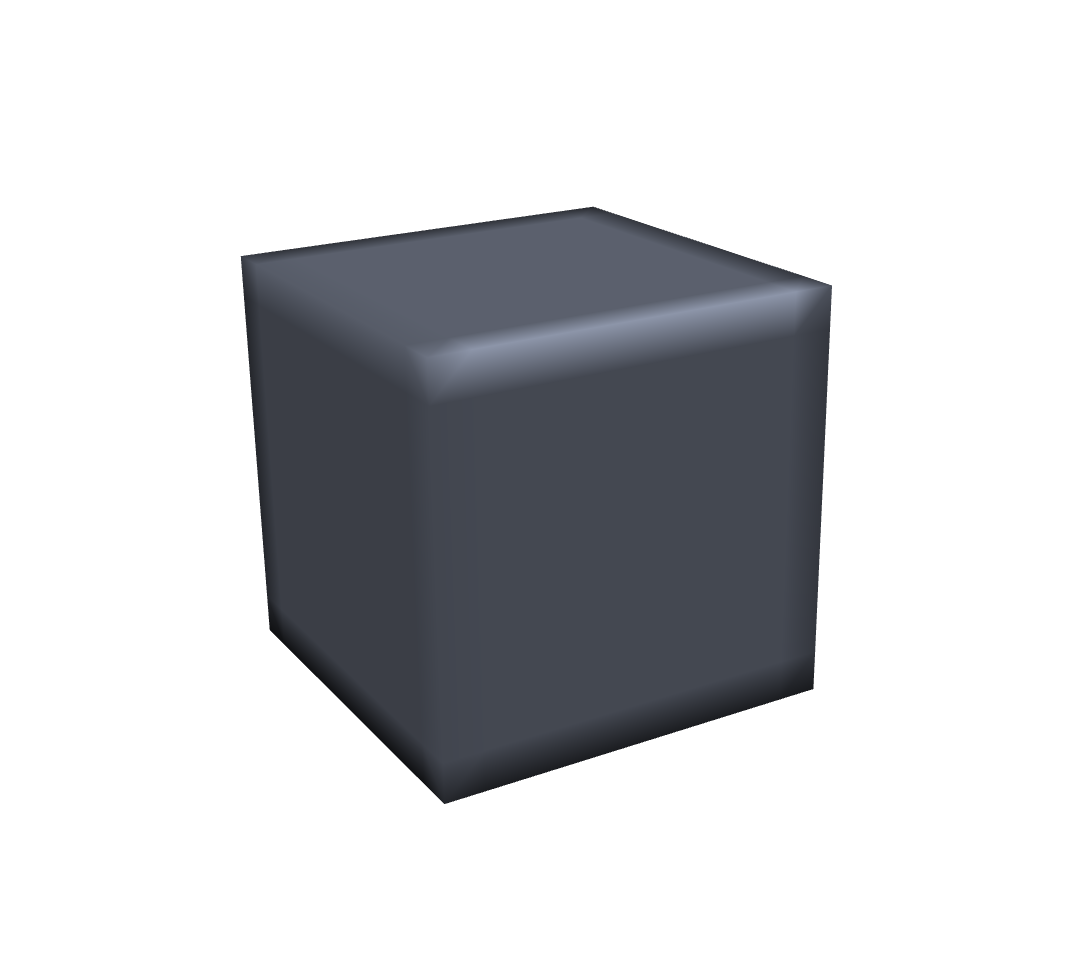
\includegraphics[width=0.32\textwidth]{resources/scramble_05_new.png}
        \caption{Results after 10, 40, and 63 Newton iterations (from left to right)}
    \end{subfigure}
    \caption{Scramble test on a cube}
    \label{fig:scramble}
\end{figure}

In Fig. \ref{fig:scramble}, we can see the solution process for 0, 1, 2, 10, 40, and finally 63 Newton iterations with $\mu=1.0$ and $\lambda = 10.0$. For this example, I had to alter the code a bit to get the desired functionalities. The initial hexahedral mesh is a cube consisting of $1'331$ vertices and $1'000$ hexahedra. Just like the authors, I fixed only four corner vertices and scrambled the remaining vertices of the cube within a space of twice the rest volume. 

The last image of Fig. \ref{fig:scramble} shows the cube back in its rest state. Hence, the model is able to recover from this extreme deformation after 63 Newton iterations. In conclusion, the model has rest stability even under these inverted configurations.

\subsection{Experiments on a more complex Mesh}
After the experiments with simple meshes as the cube and cylinder, it would be interesting to see how the energy performs on a more complex mesh. For the following two experiments, I chose a tetrahedral mesh consisting of $5'650$ vertices and $20'203$ tetrahedra. The mesh is formed in the shape of a bird. Fig. \ref{fig:bird} shows the object in its rest state from different angles.
\begin{figure}[!htbp]
	\centering
	\begin{subfigure}[b]{\textwidth}
        \centering
        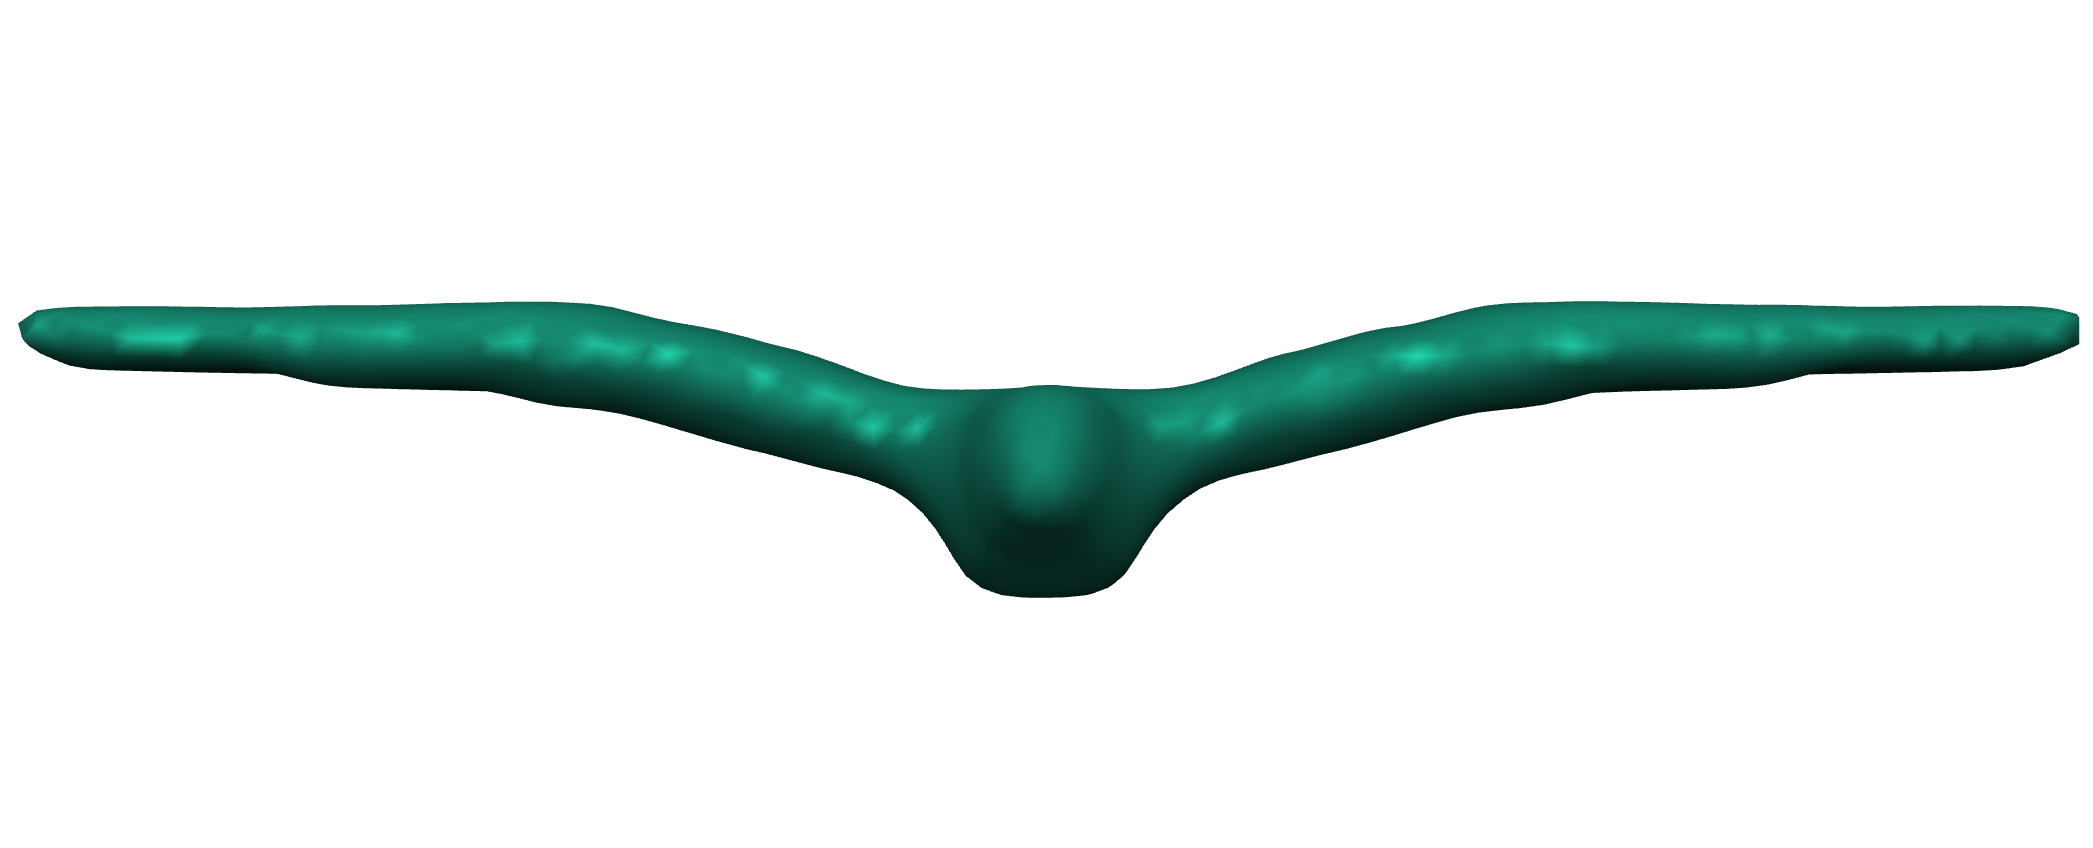
\includegraphics[width=0.44\textwidth]{resources/bird_front.png}
        \hfill
        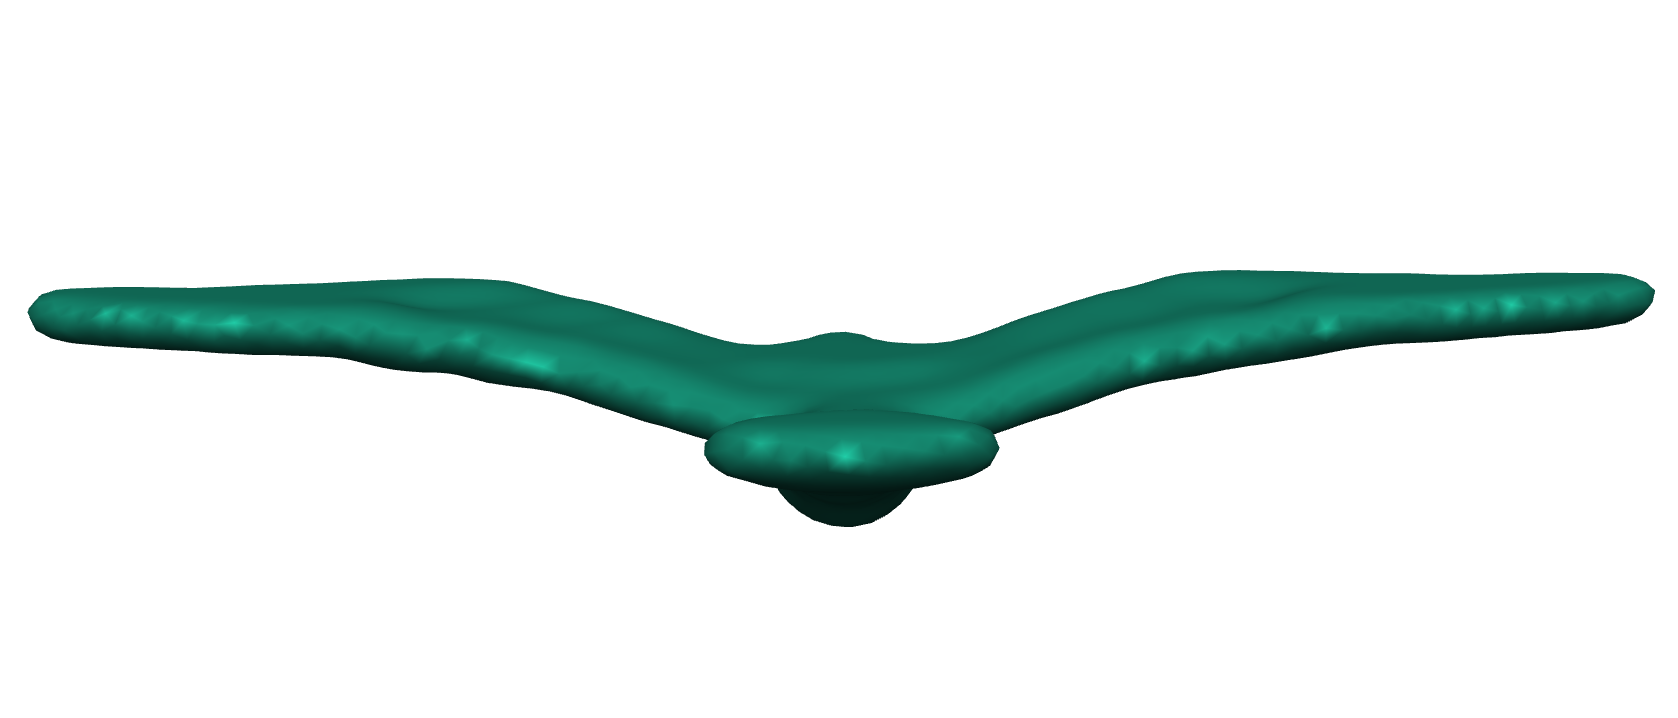
\includegraphics[width=0.44\textwidth]{resources/bird_back.png}
        \caption{Front and back of the mesh (from left to right)}
    \end{subfigure}
    \vskip\baselineskip
    \begin{subfigure}[b]{\textwidth}
        \centering
        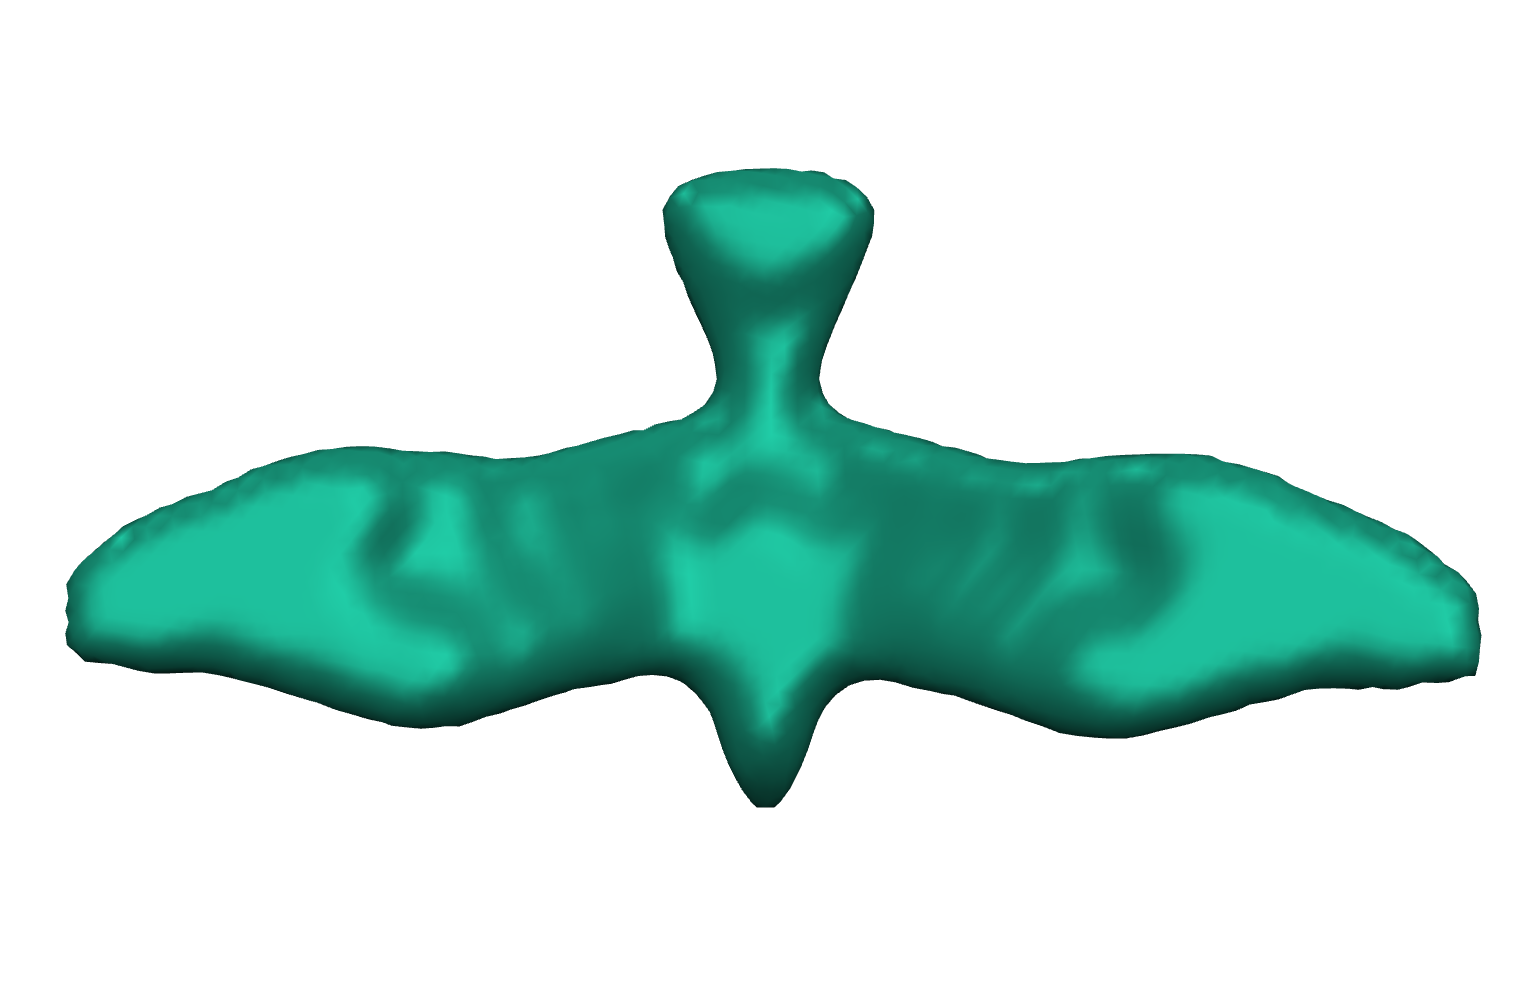
\includegraphics[width=0.44\textwidth]{resources/bird_above.png}
        \hfill
        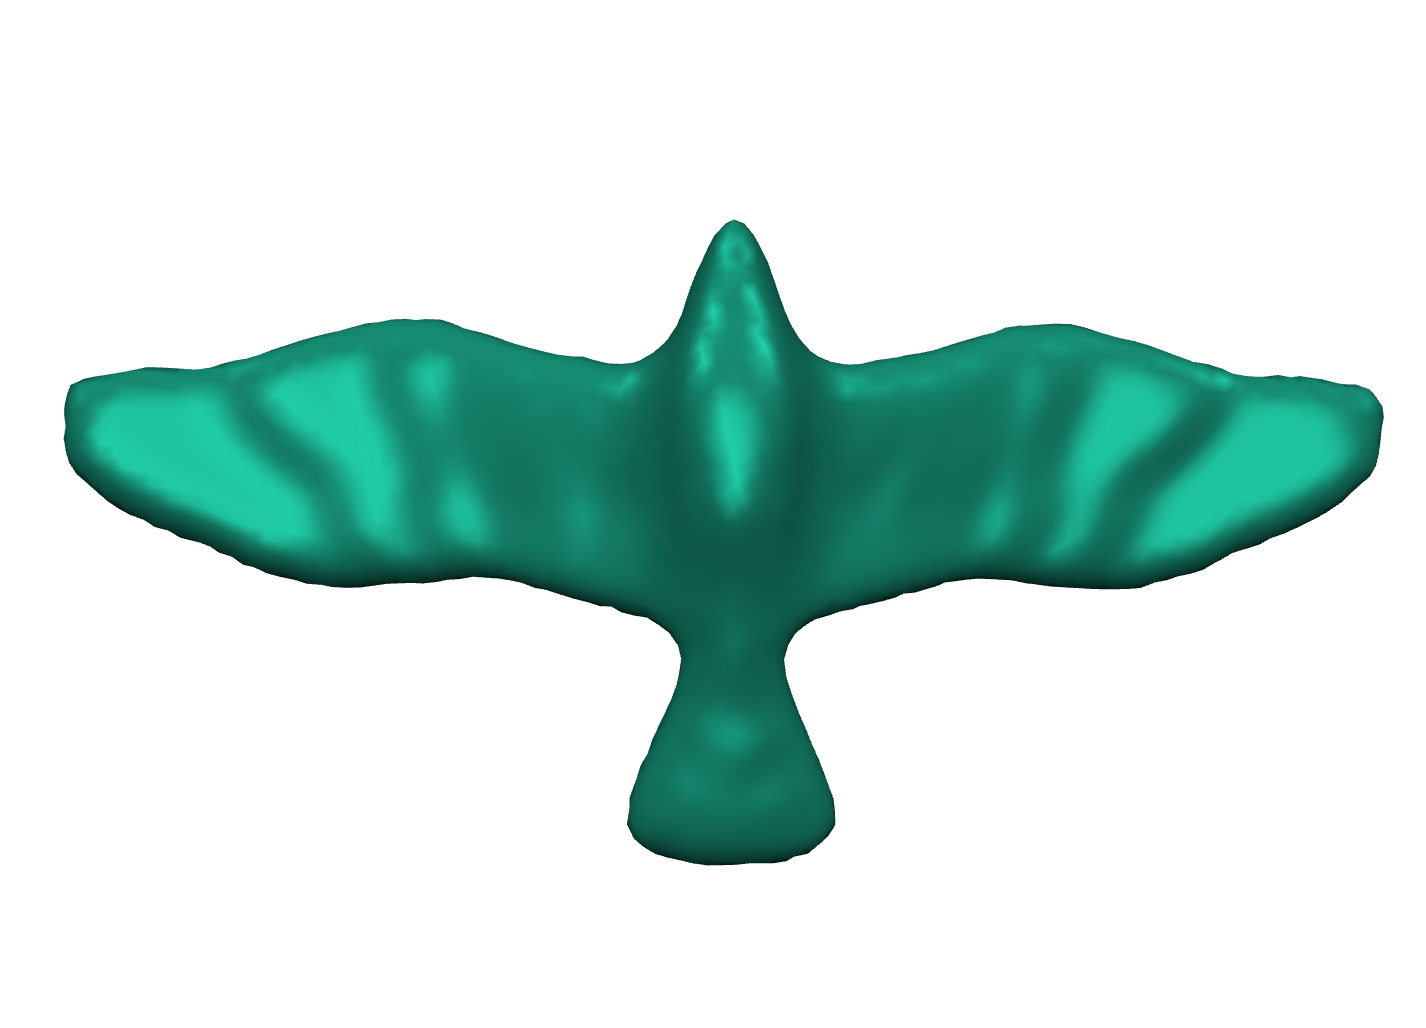
\includegraphics[width=0.44\textwidth]{resources/bird_bottom.png} 
        \caption{Top and bottom of the mesh (from left to right)}
    \end{subfigure}
    \caption{Object in its rest state shown from different angles}
    \label{fig:bird}
\end{figure}

For the first deformation, I stretched the bird in four directions: along the left and right wing, the head, and tail. That will give us an extreme stretch to further test the energy. For the parameters, I set $\lambda$ equal to $10.0$, $\mu$ equal to $1.0$, and the step size equal to $0.01$. The result of this deformation after ten steps is shown in Fig. \ref{fig:bird_deformed_stretched}.
\begin{figure}[!htbp]
	\centering
	\begin{subfigure}[b]{\textwidth}
        \centering
        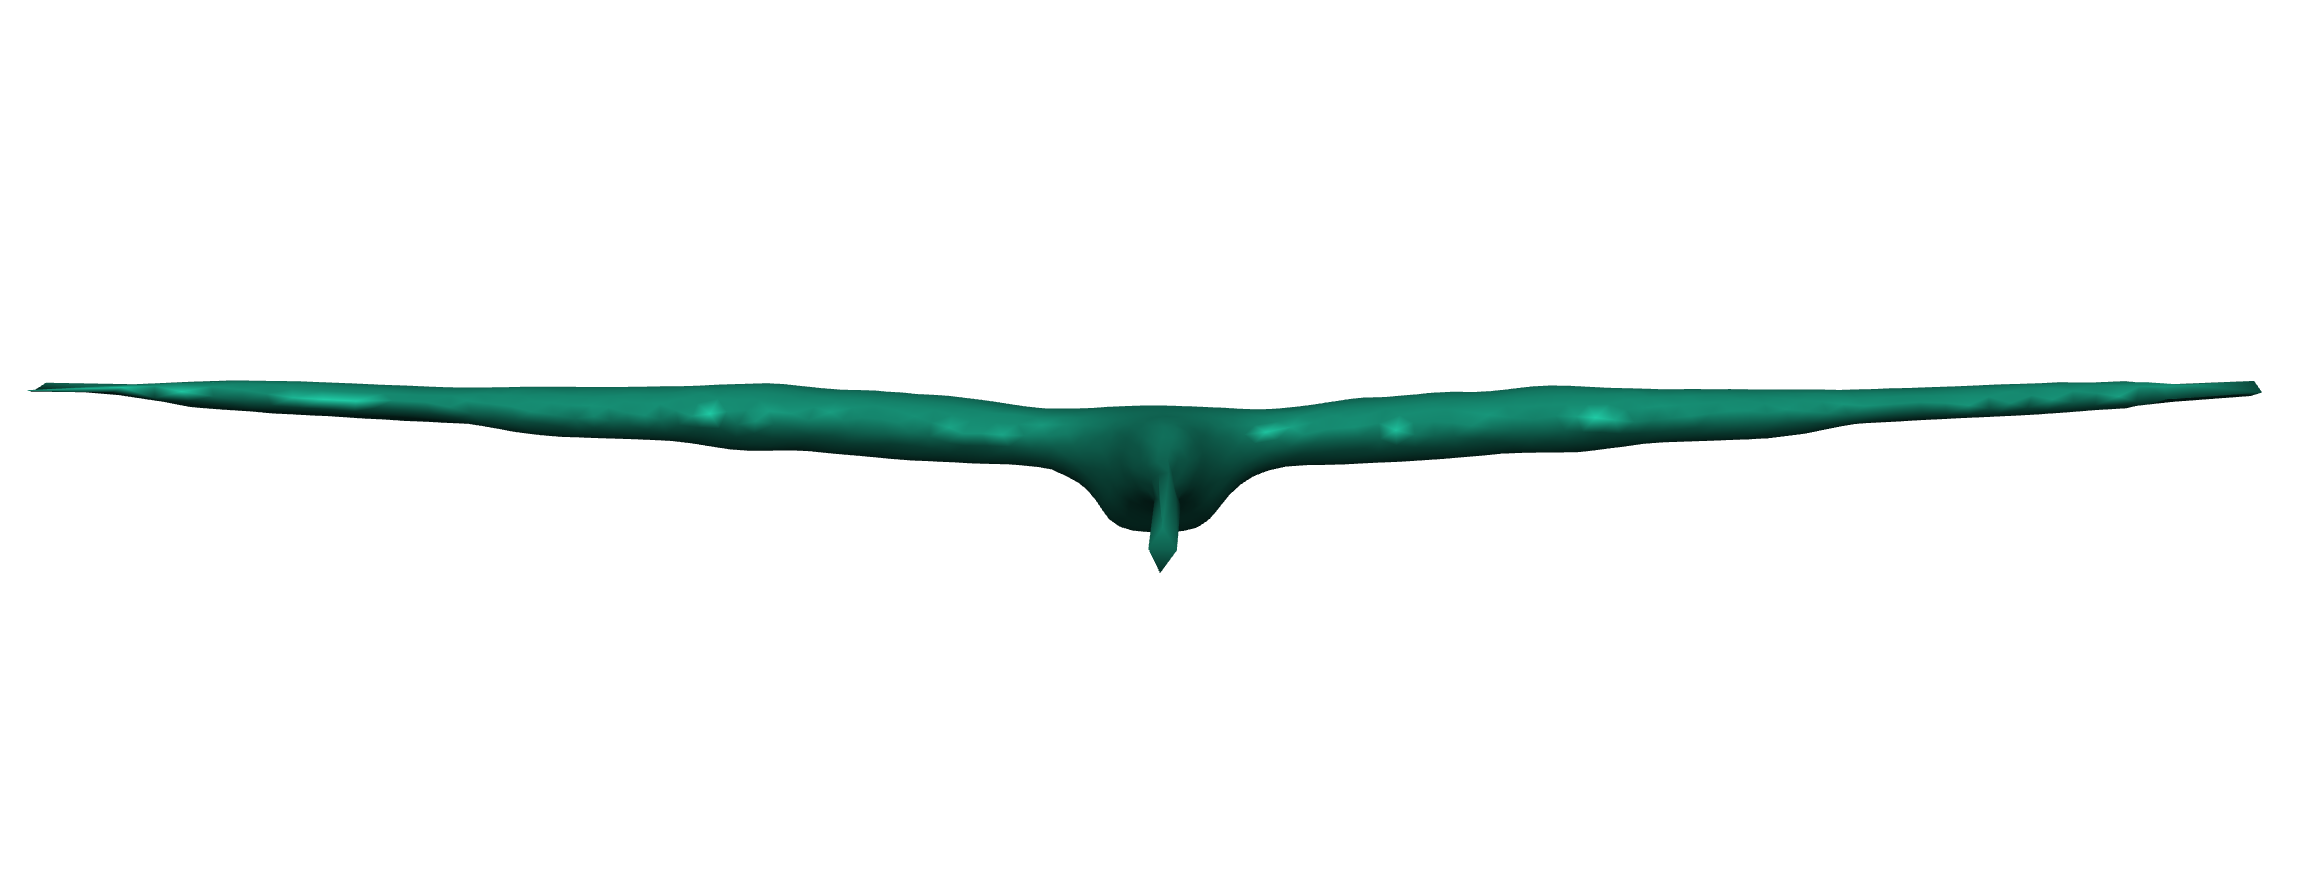
\includegraphics[width=0.44\textwidth]{resources/stretched_front.png}
        \hfill
        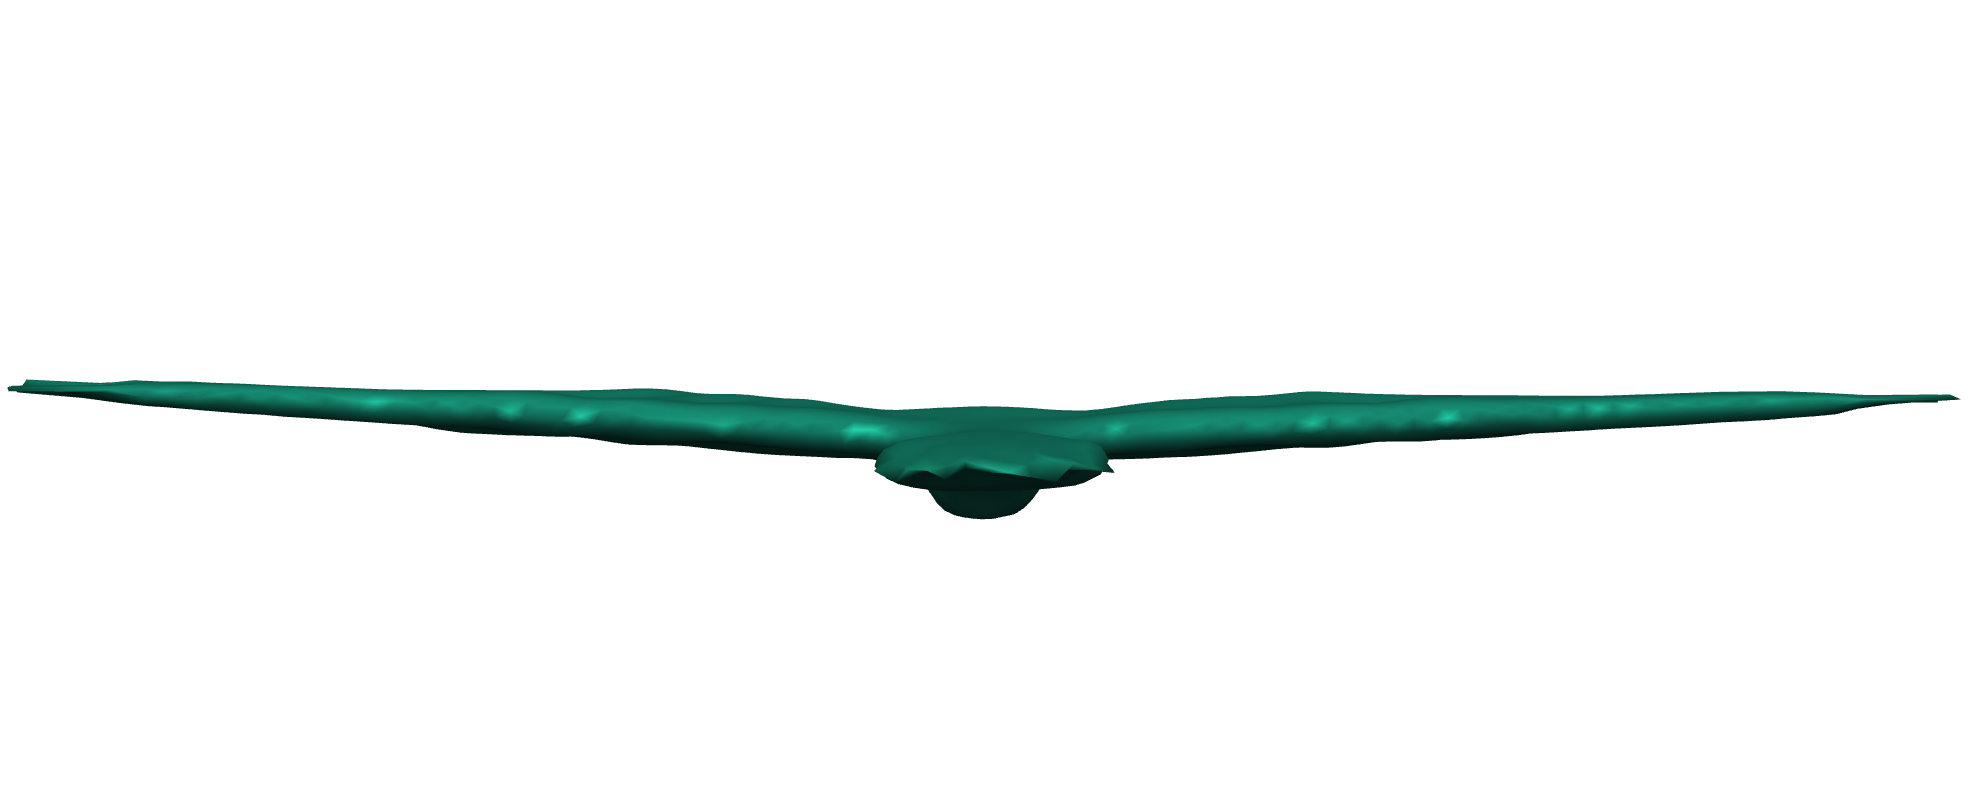
\includegraphics[width=0.44\textwidth]{resources/stretched_back.png}
        \caption{Front and back of the mesh (from left to right)}
    \end{subfigure}
    \vskip\baselineskip
    \begin{subfigure}[b]{\textwidth}
        \centering
        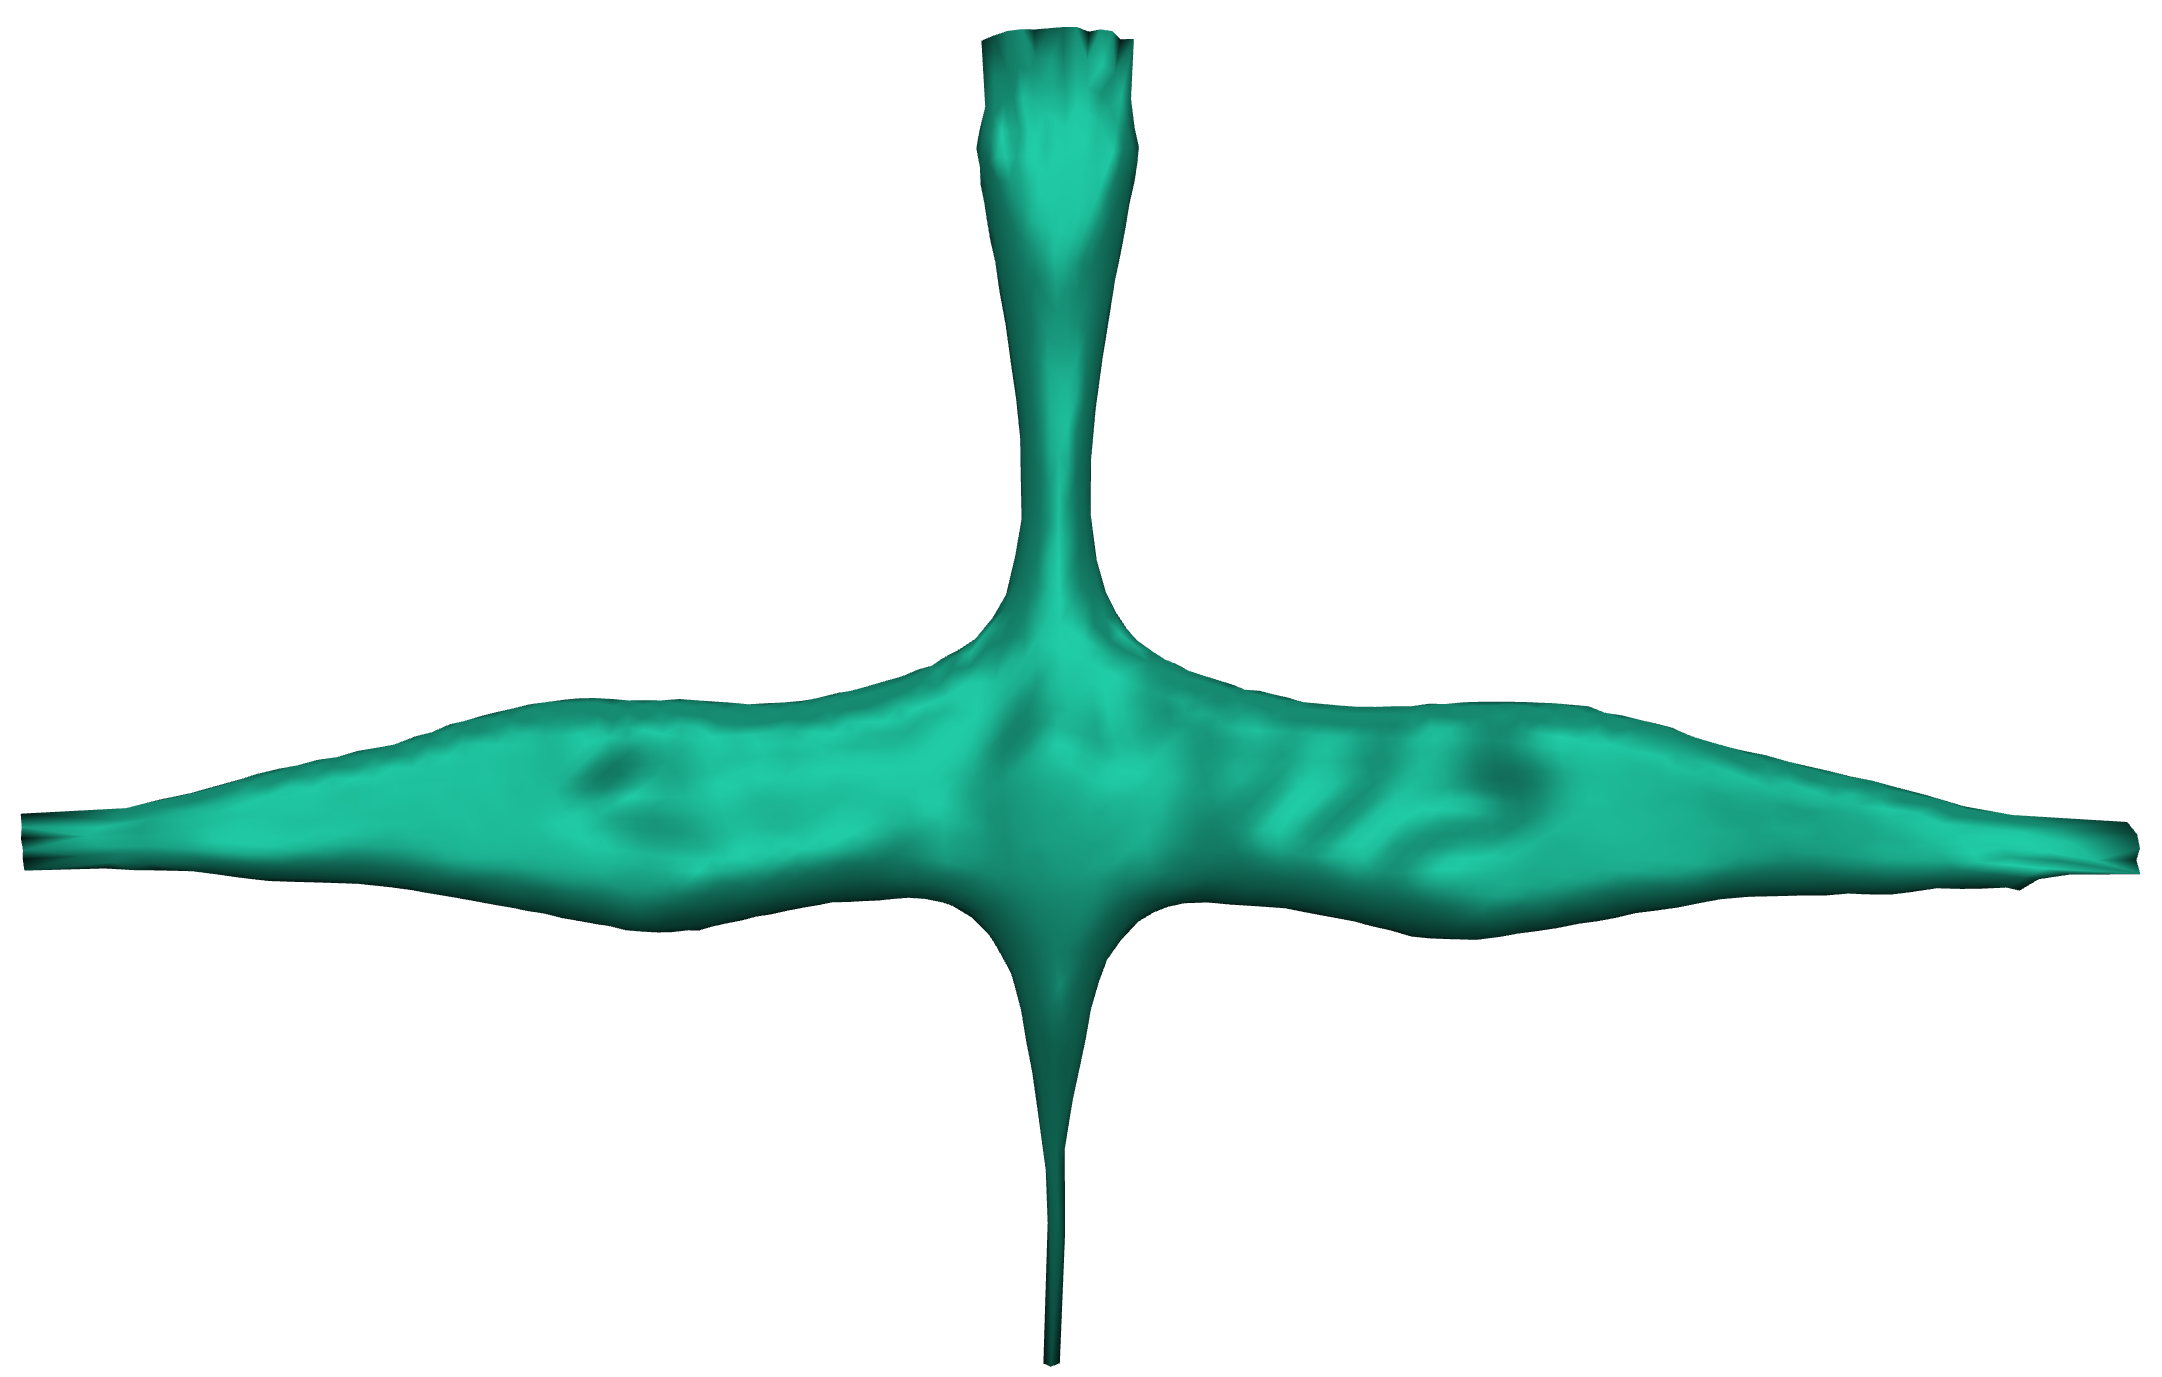
\includegraphics[width=0.44\textwidth]{resources/stretched_top.png}
        \hfill
        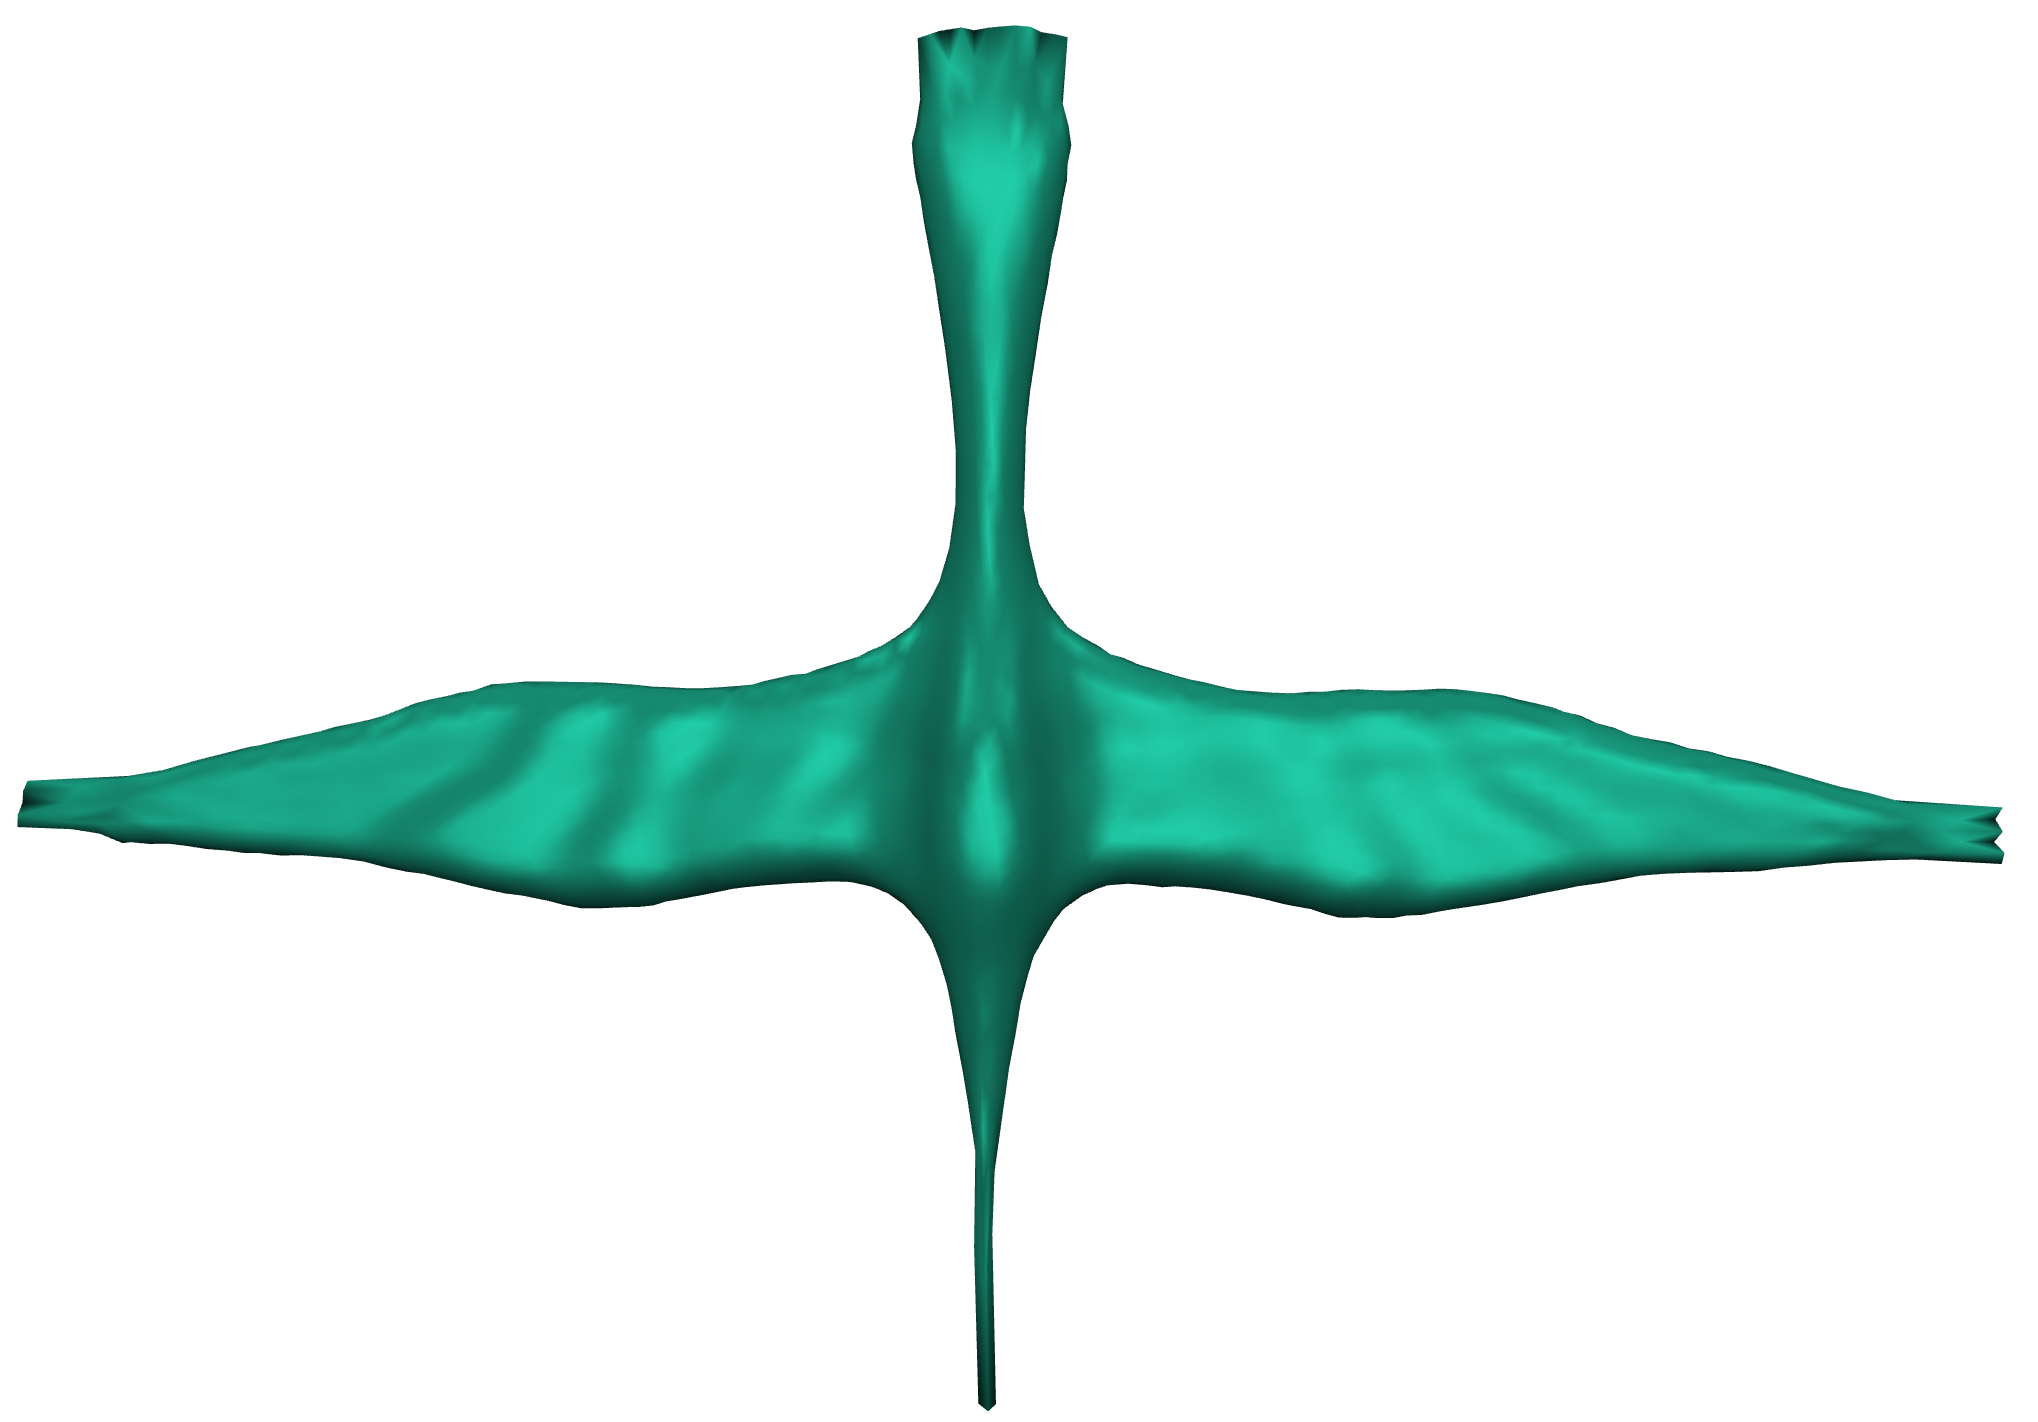
\includegraphics[width=0.44\textwidth]{resources/stretched_bottom.png}
        \caption{Top and bottom of the mesh (from left to right)}
    \end{subfigure}
    \caption{Stretched object shown from different angles}
    \label{fig:bird_deformed_stretched}
\end{figure}

As we can see, the wings lost their bend with this extreme stretch, and the head has become almost a straight line. Overall, the deformed object looks as good as it can under these extreme conditions, and the energy behaves well. There are some places where we can imagine which vertices I pulled to perform the stretch. For example, Fig. \ref{fig:bird_deformed_stretched_zigzag} shows how the outer part of the wings form almost a zig-zag pattern. Unfortunately, that was unavoidable because of the configuration of the mesh. If the vertices were aligned in a straight line, this effect would not be seen.
\begin{figure}[!htbp]
	\centering
	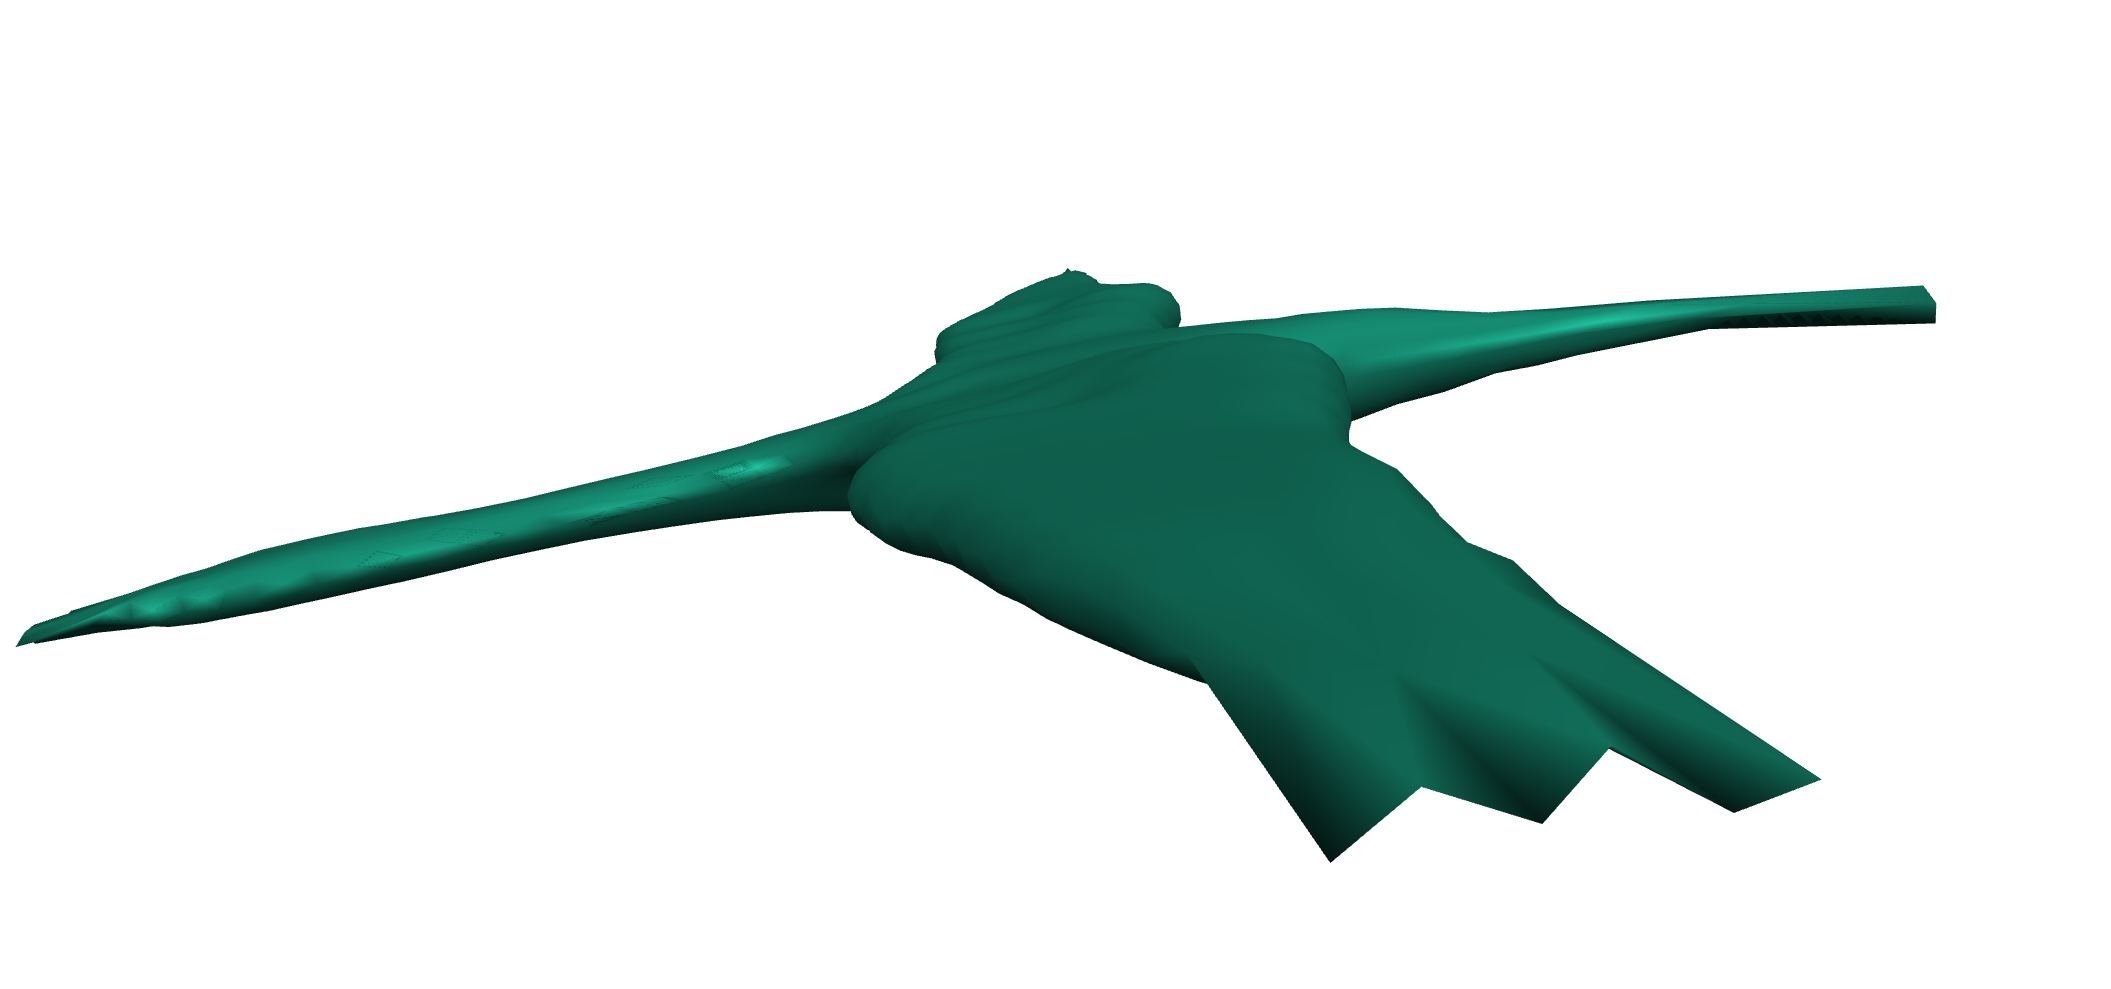
\includegraphics[width=0.44\textwidth]{resources/stretched_zigzag.png}
    \caption{Irregularity on the right wing (from the bird's point of view)}
    \label{fig:bird_deformed_stretched_zigzag}
\end{figure}

Additionally, instead of just stretching the object, we should also test how the energy behaves for other deformations. For the next experiment with this mesh, I pushed the two wings together and pulled the body down. With this configuration, we can bend the wings and see how the energy behaves under these conditions. Again, I set $\lambda$ equal to $10.0$, $\mu$ equal to $1.0$, and the step size equal to $0.01$
Fig. \ref{fig:bird_deformed_bend} shows the deformed object after ten steps.
\begin{figure}[!htbp]
	\centering
	\begin{subfigure}[b]{\textwidth}
        \centering
        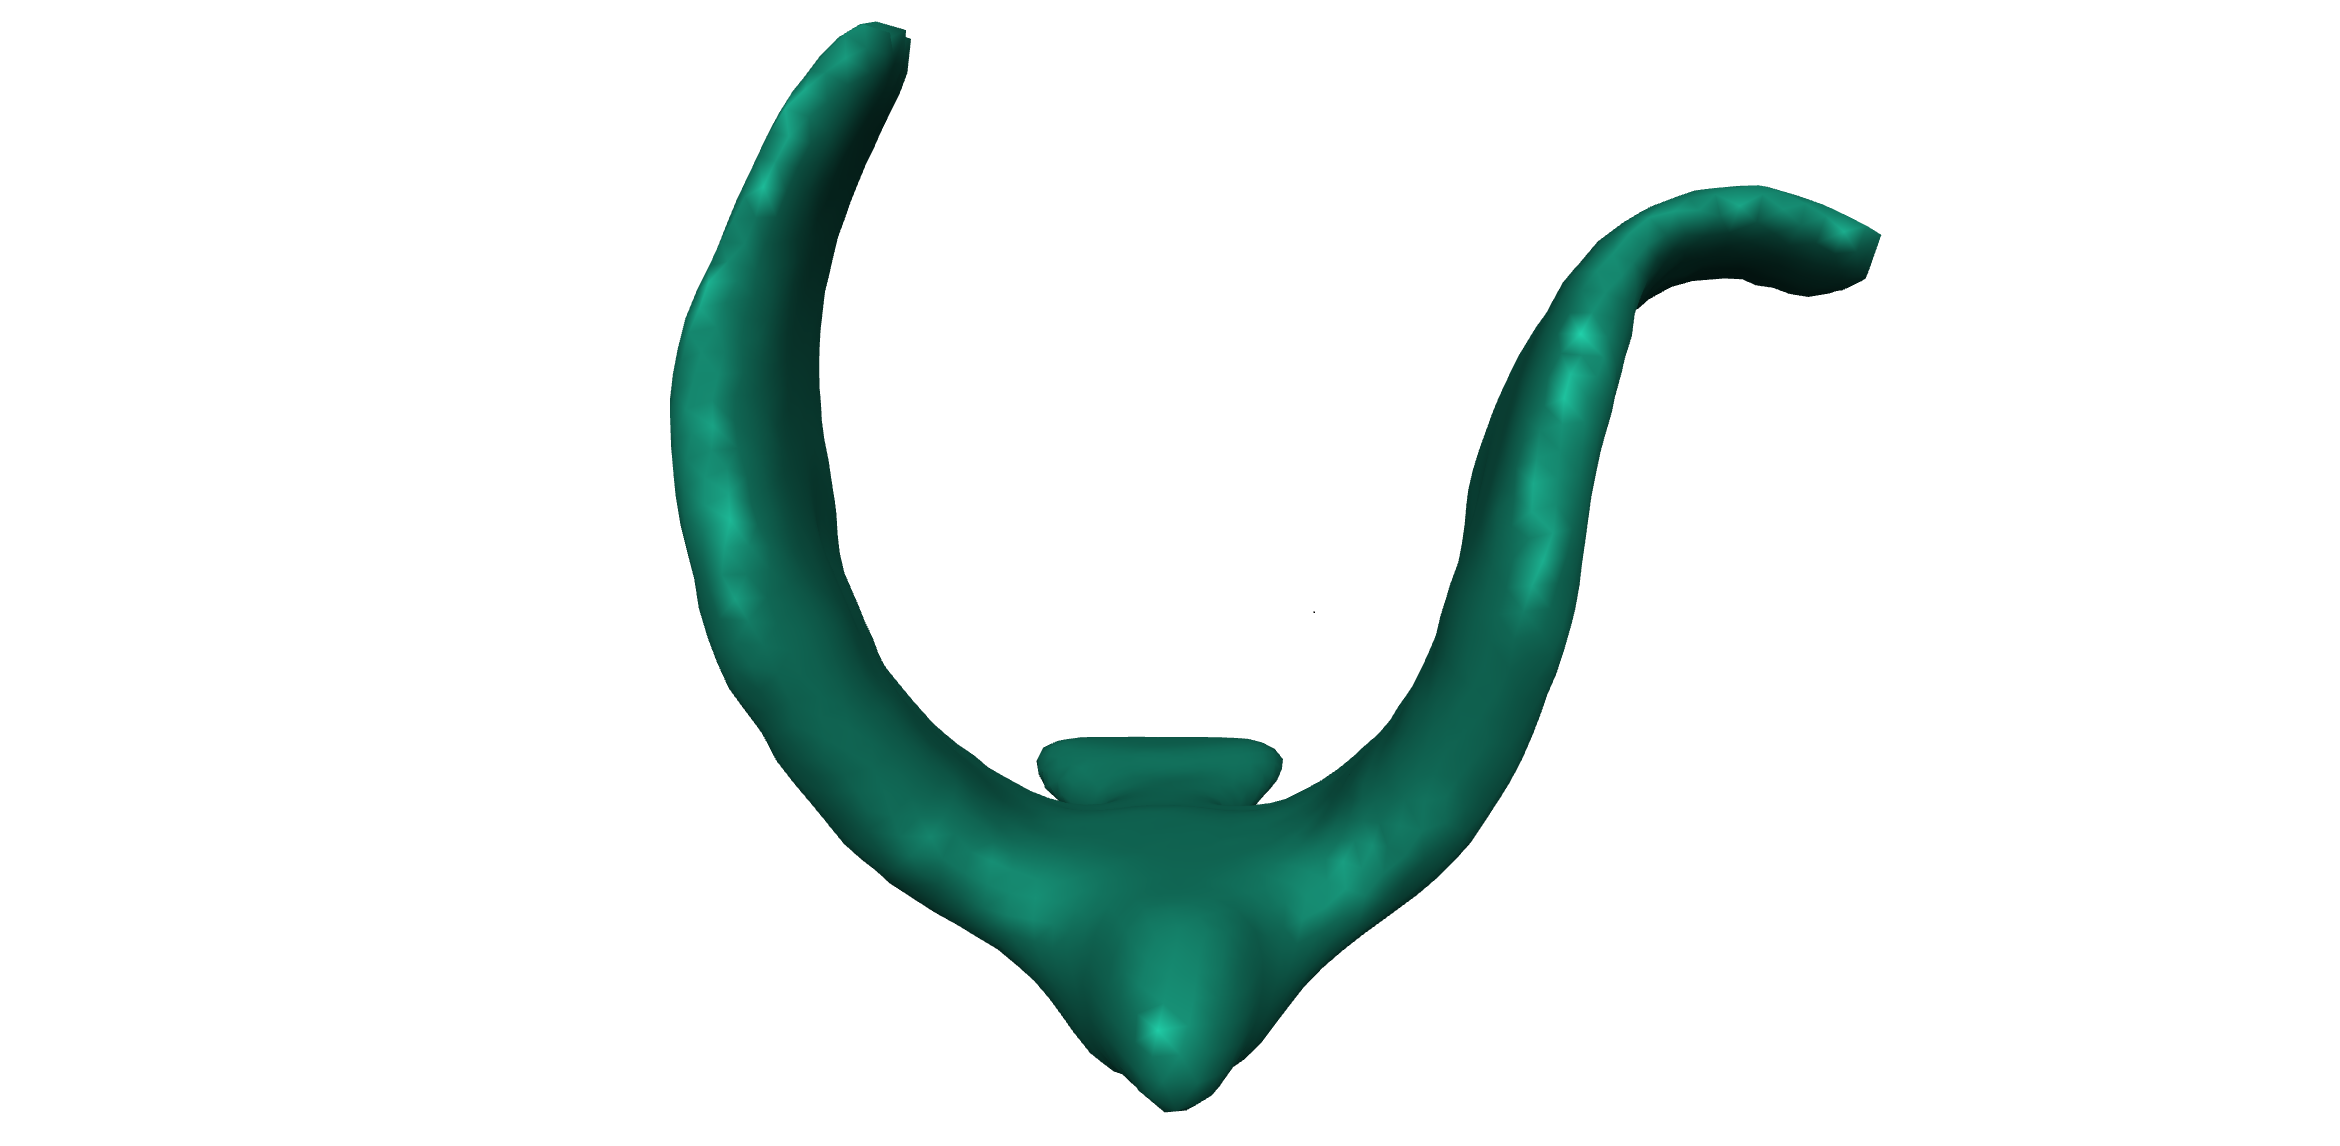
\includegraphics[width=0.44\textwidth]{resources/bent_front.png}
        \hfill
        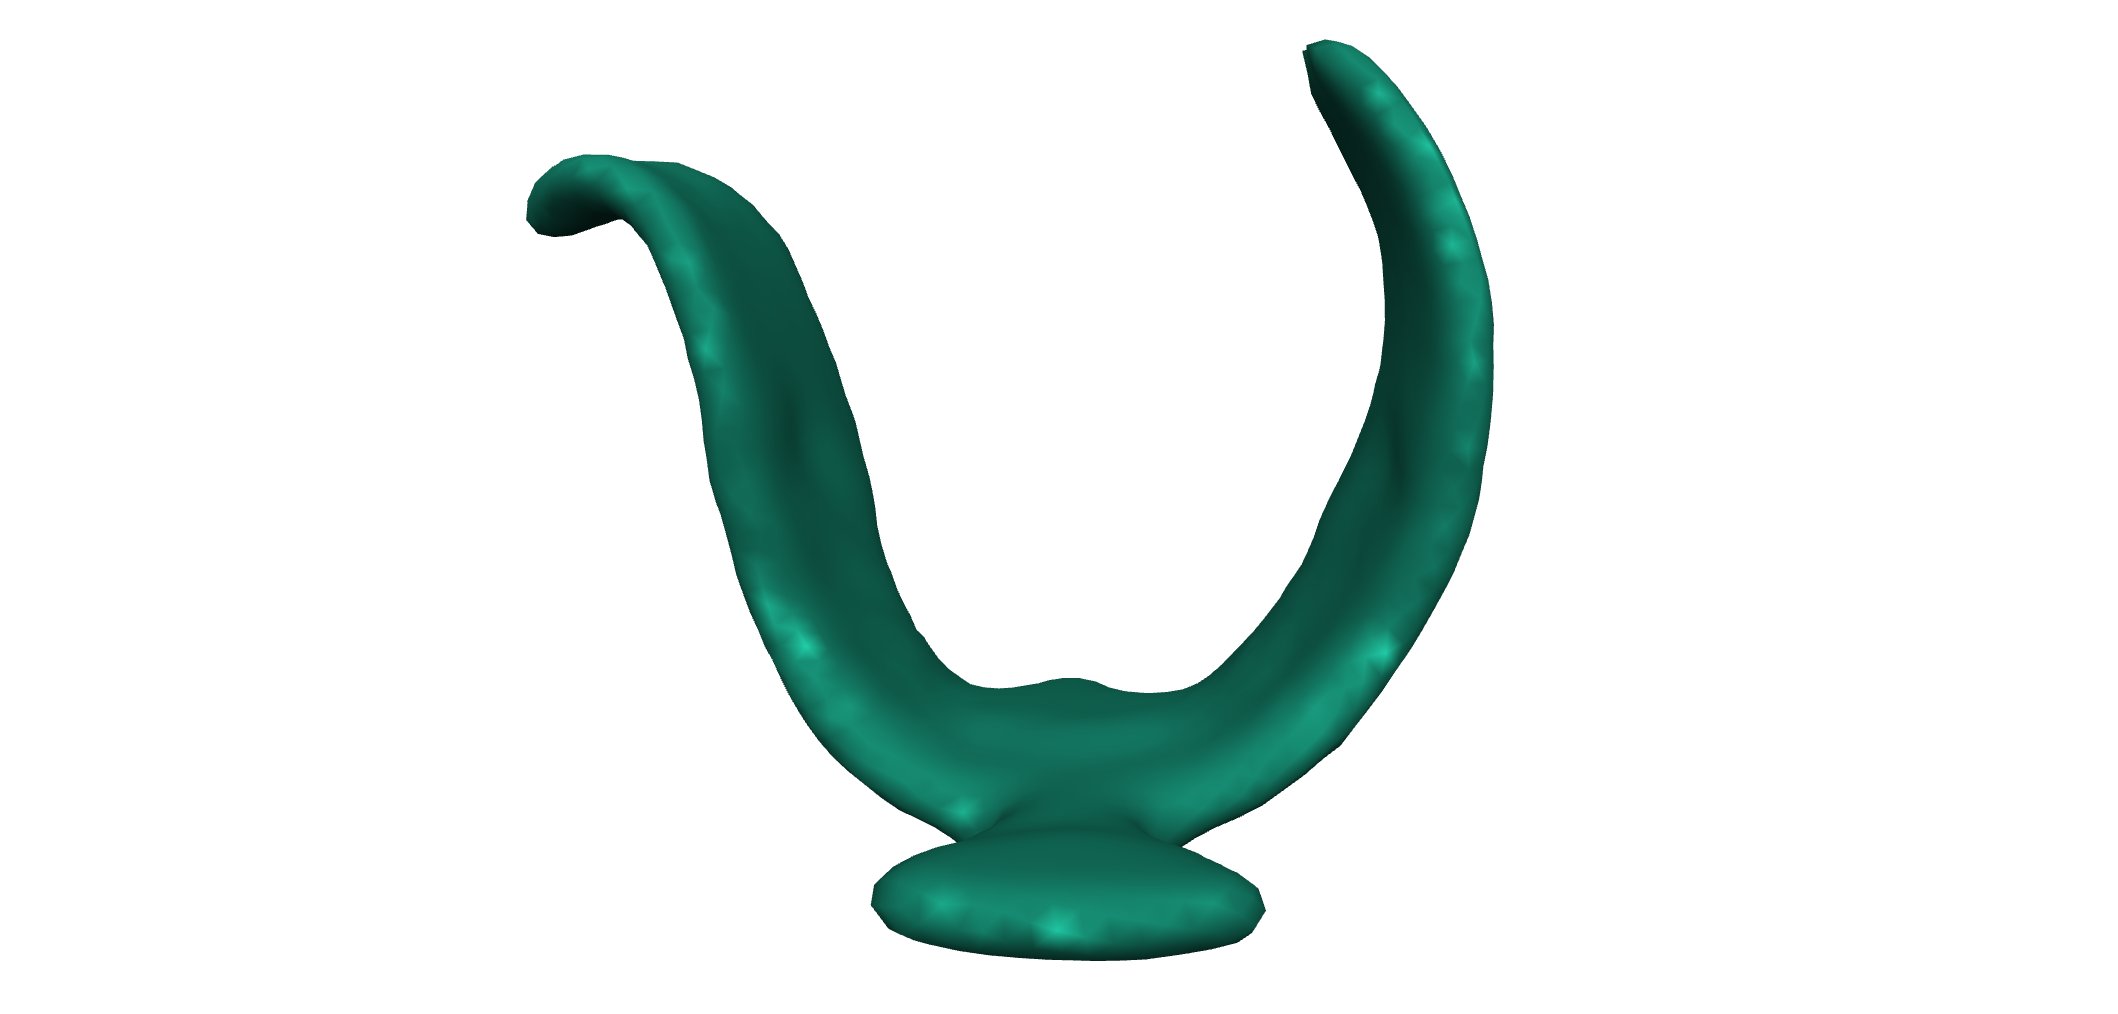
\includegraphics[width=0.44\textwidth]{resources/bent_back.png}
        \caption{Front and back of the mesh (from left to right)}
    \end{subfigure}
    \vskip\baselineskip
    \begin{subfigure}[b]{\textwidth}
        \centering
        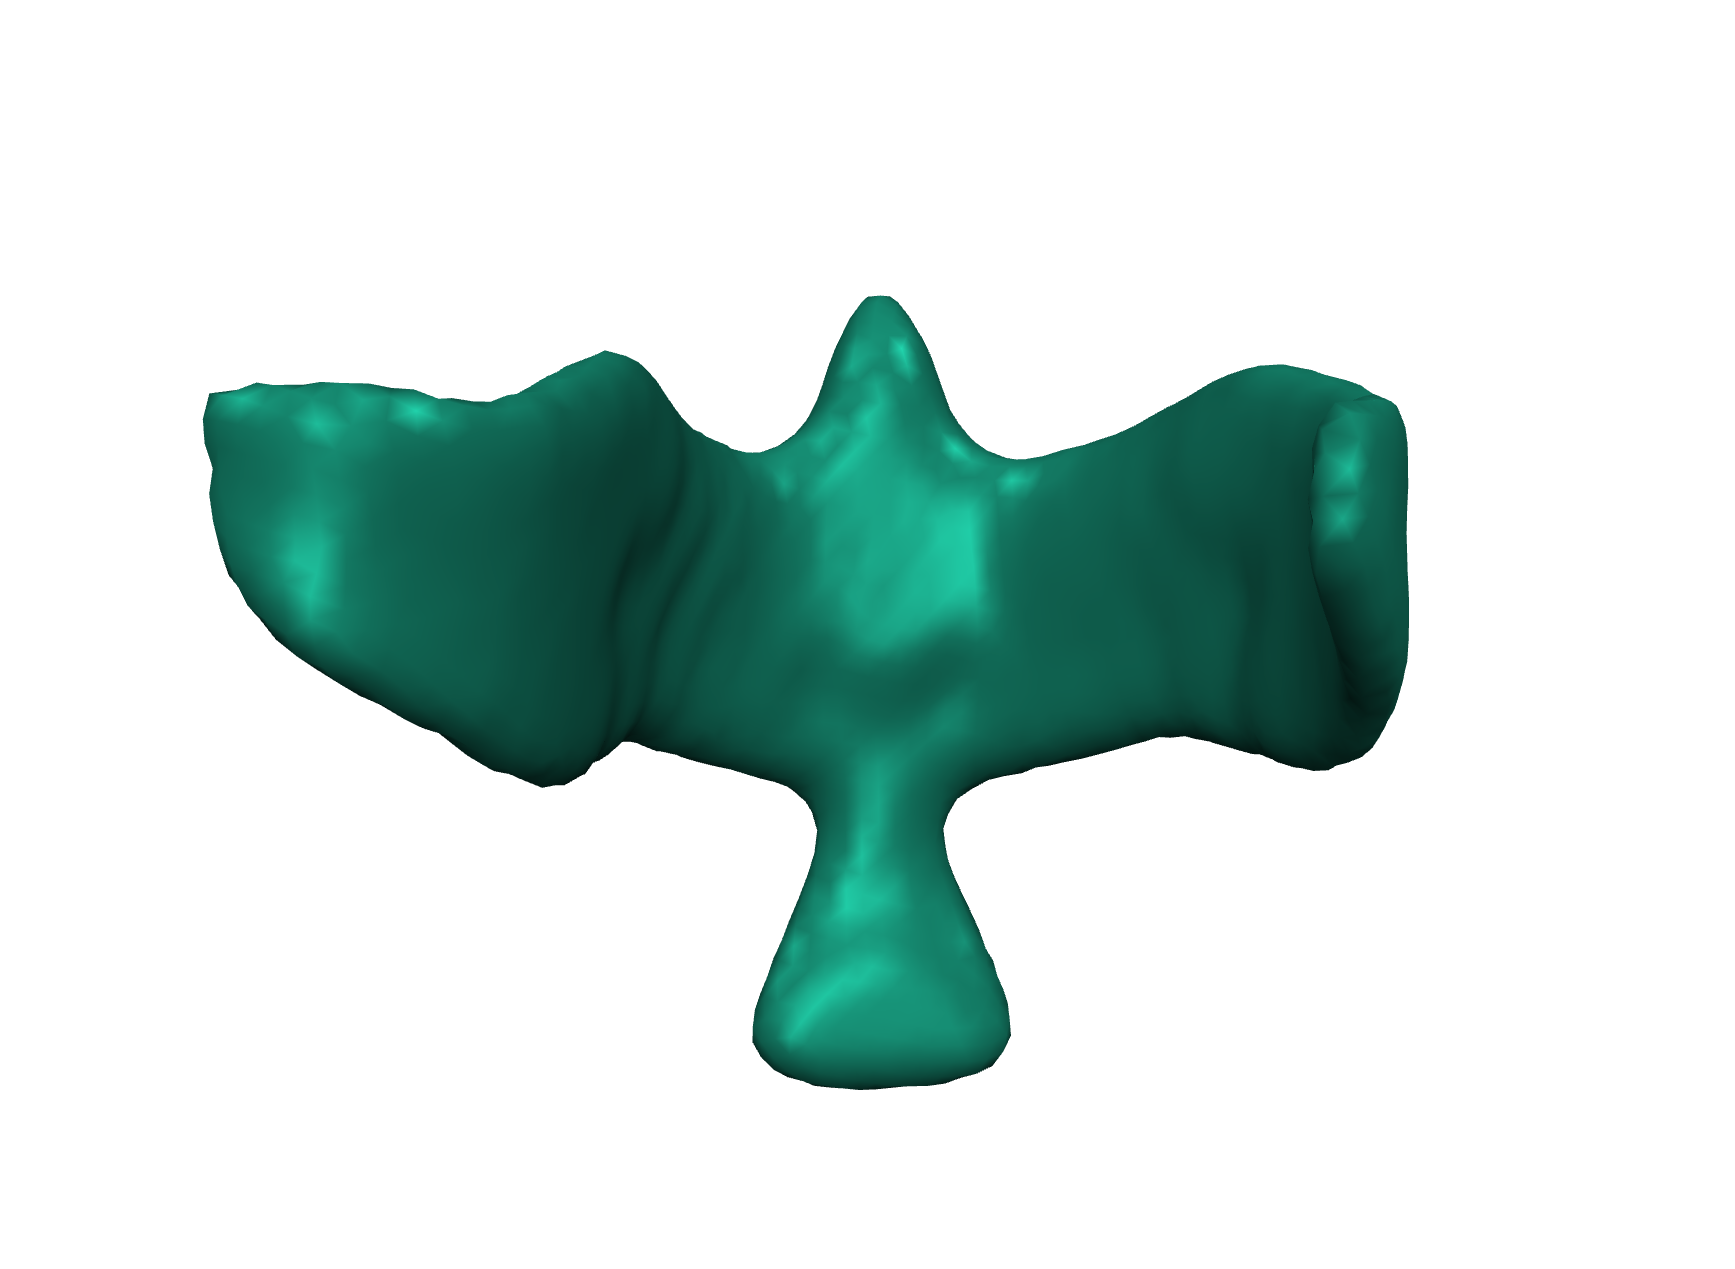
\includegraphics[width=0.44\textwidth]{resources/bent_top.png}
        \hfill
        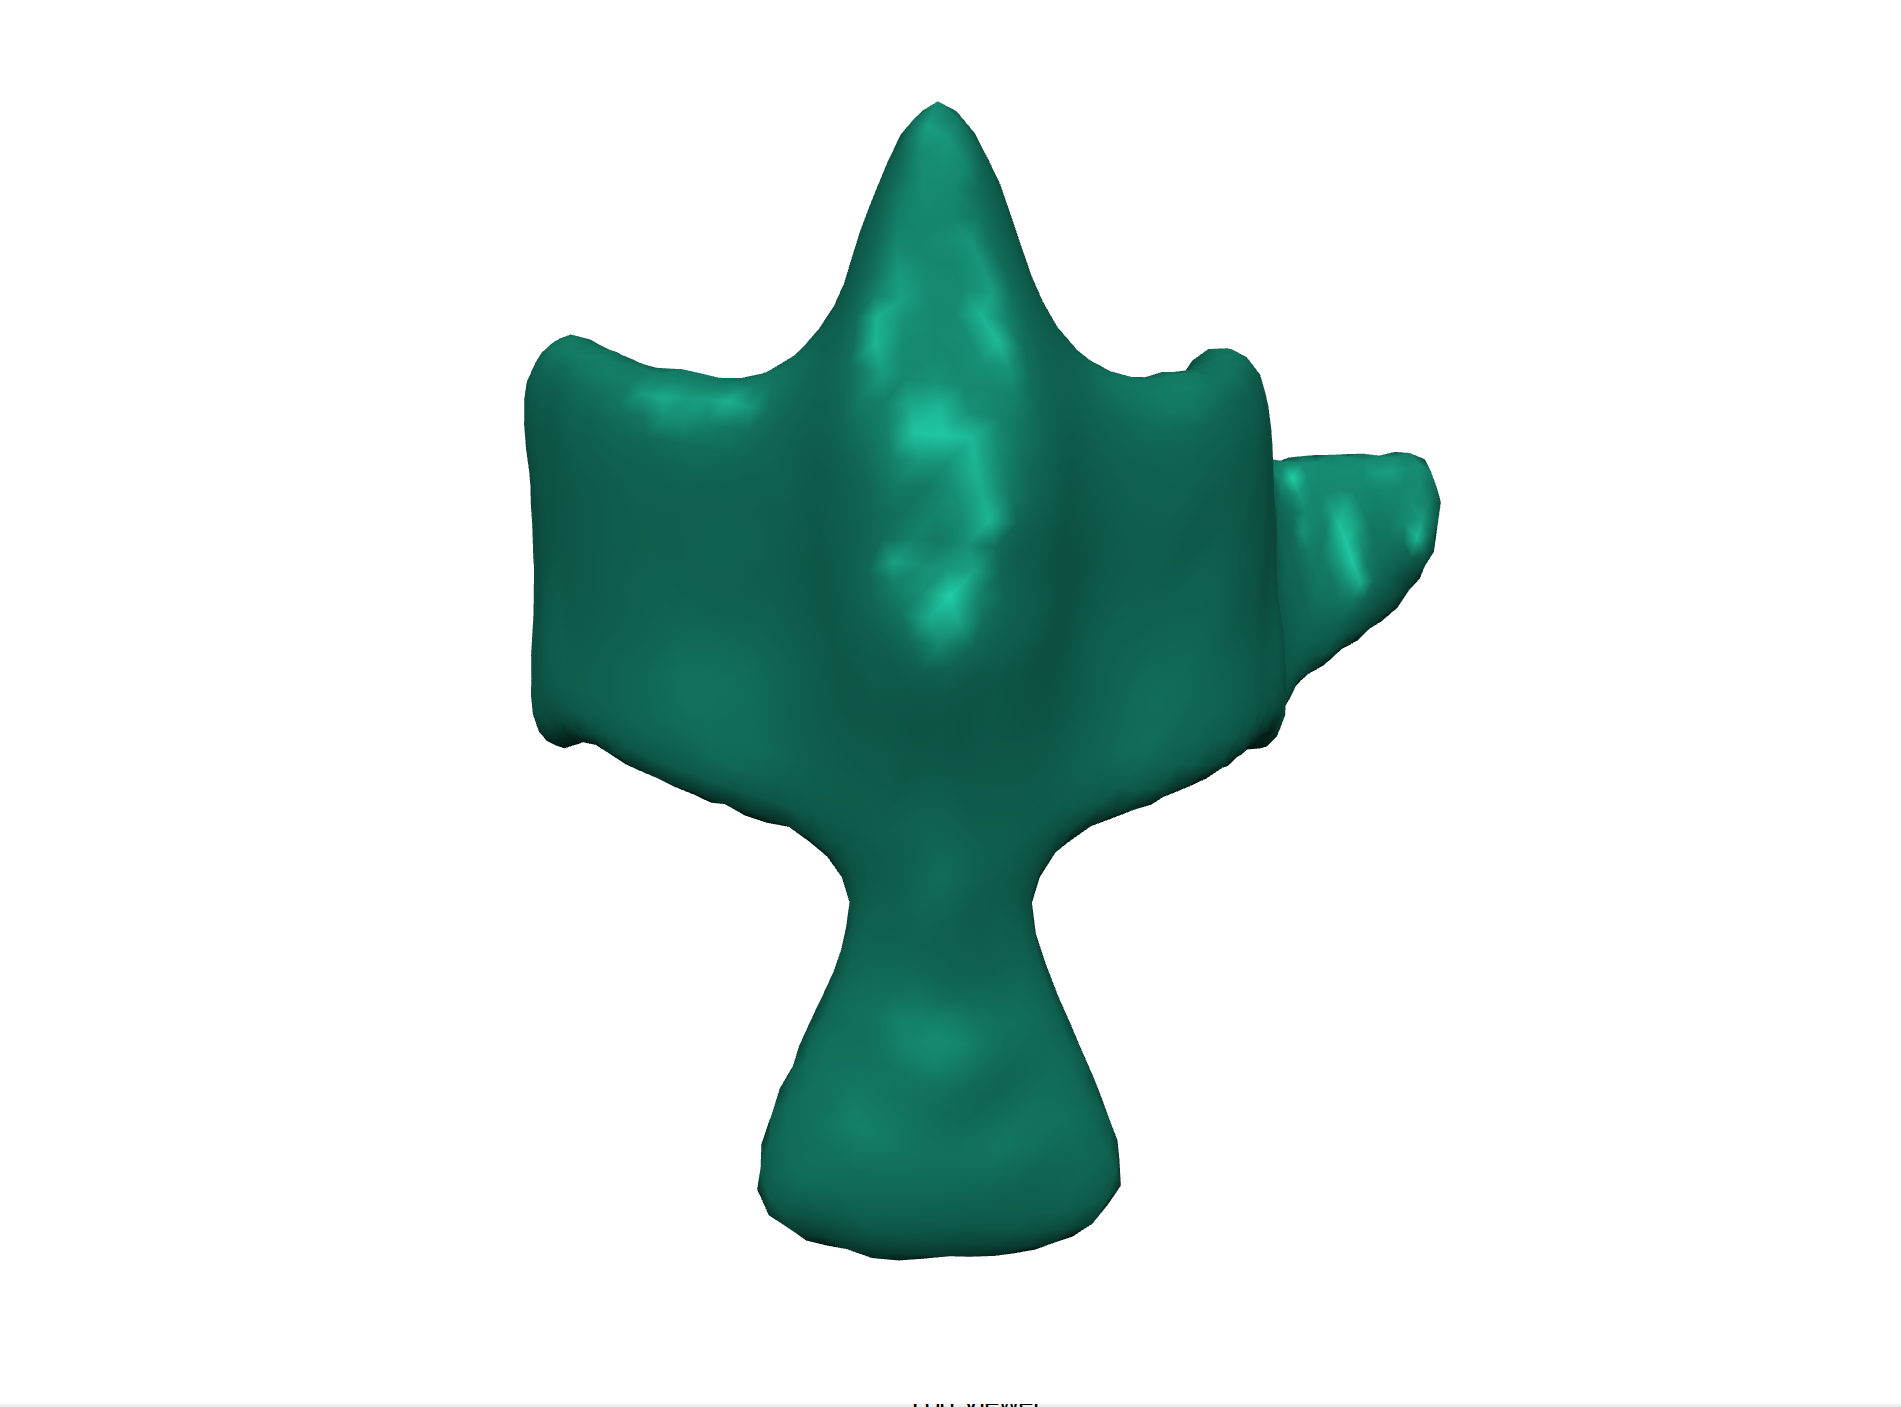
\includegraphics[width=0.44\textwidth]{resources/bent_bottom.png} 
        \caption{Top and bottom of the mesh (from left to right)}
    \end{subfigure}
    \caption{Bent object shown from different angles}
    \label{fig:bird_deformed_bend}
\end{figure}

In the images, we can see that the two wings bend differently, which is caused by the selection of vertices to pull. Fig. \ref{fig:bird_deformed_bend_side} shows the deformed object from both sides to get a better look at the deformation.
\begin{figure}[!htbp]
	\centering
    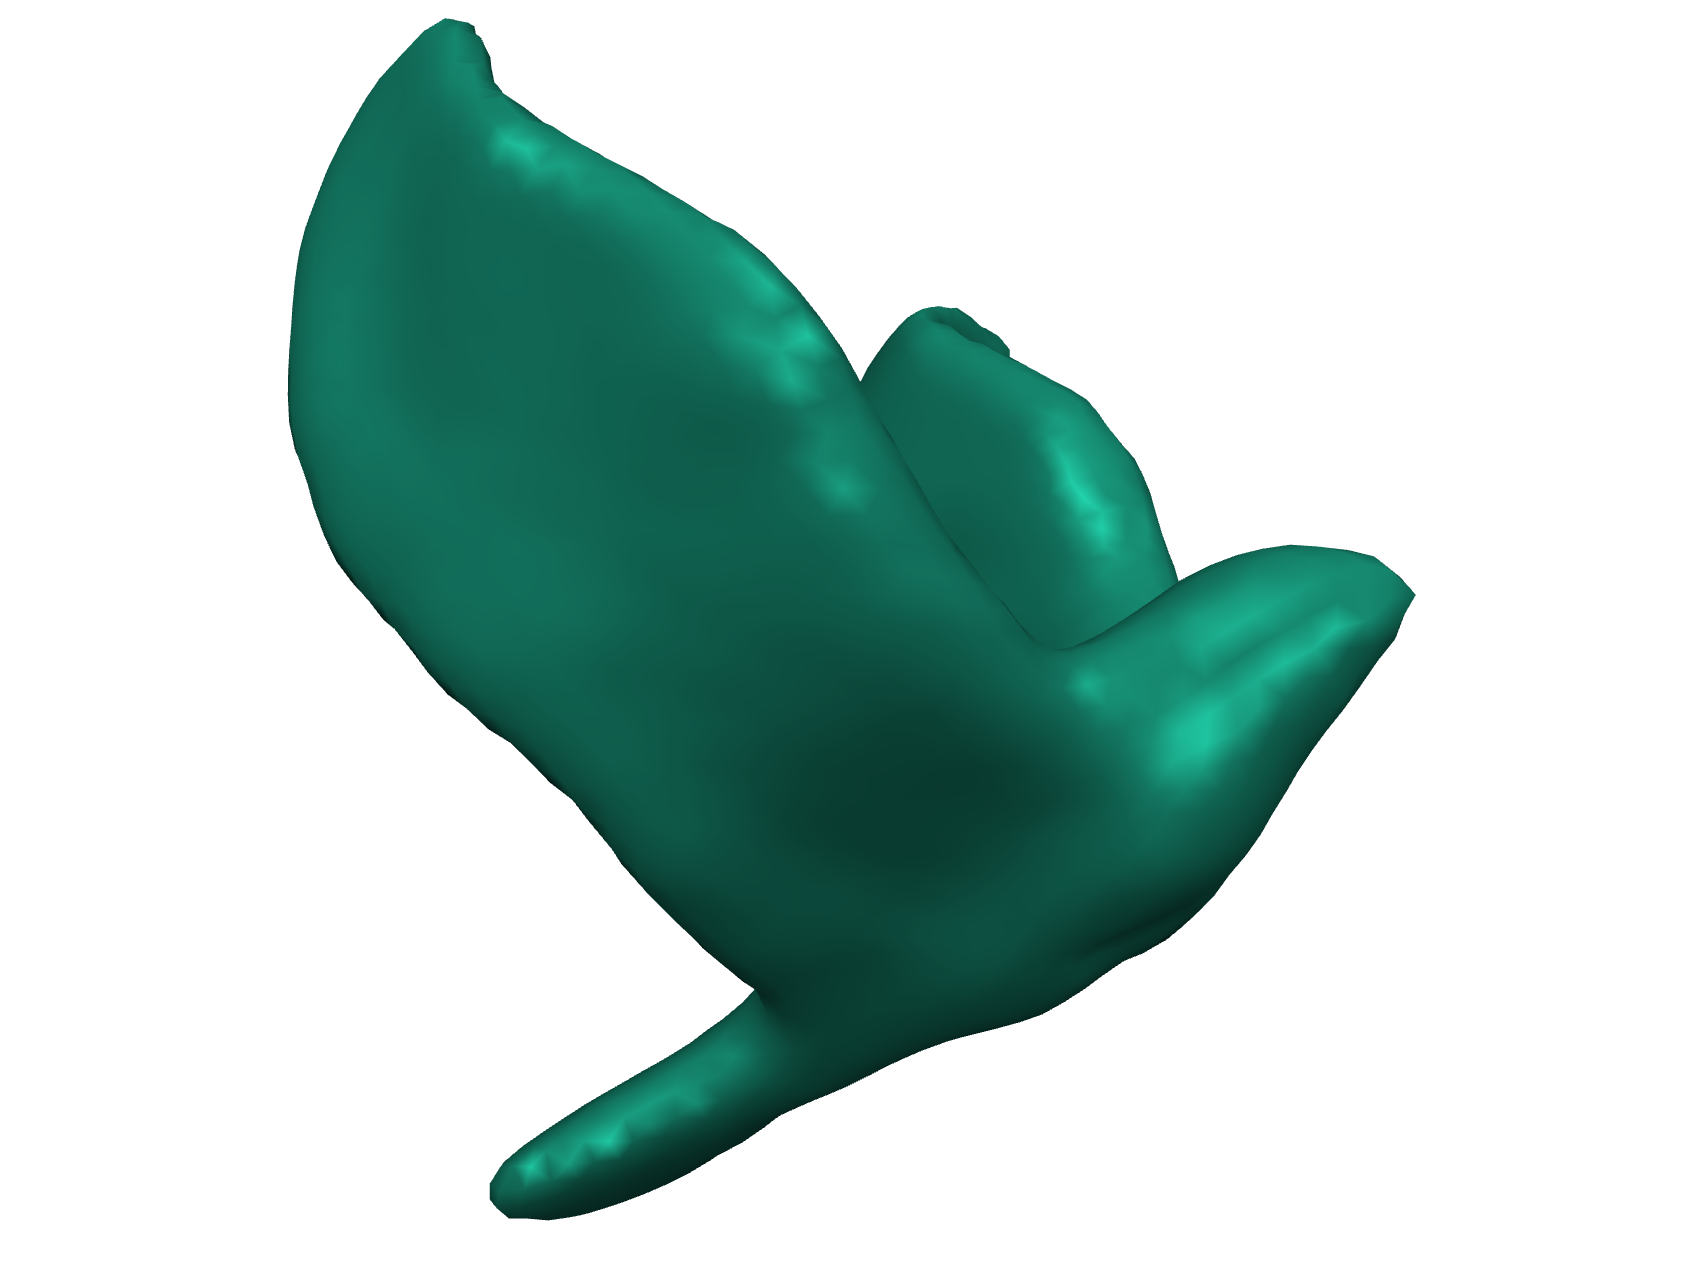
\includegraphics[width=0.44\textwidth]{resources/bent_side2.png}
    \hfill
    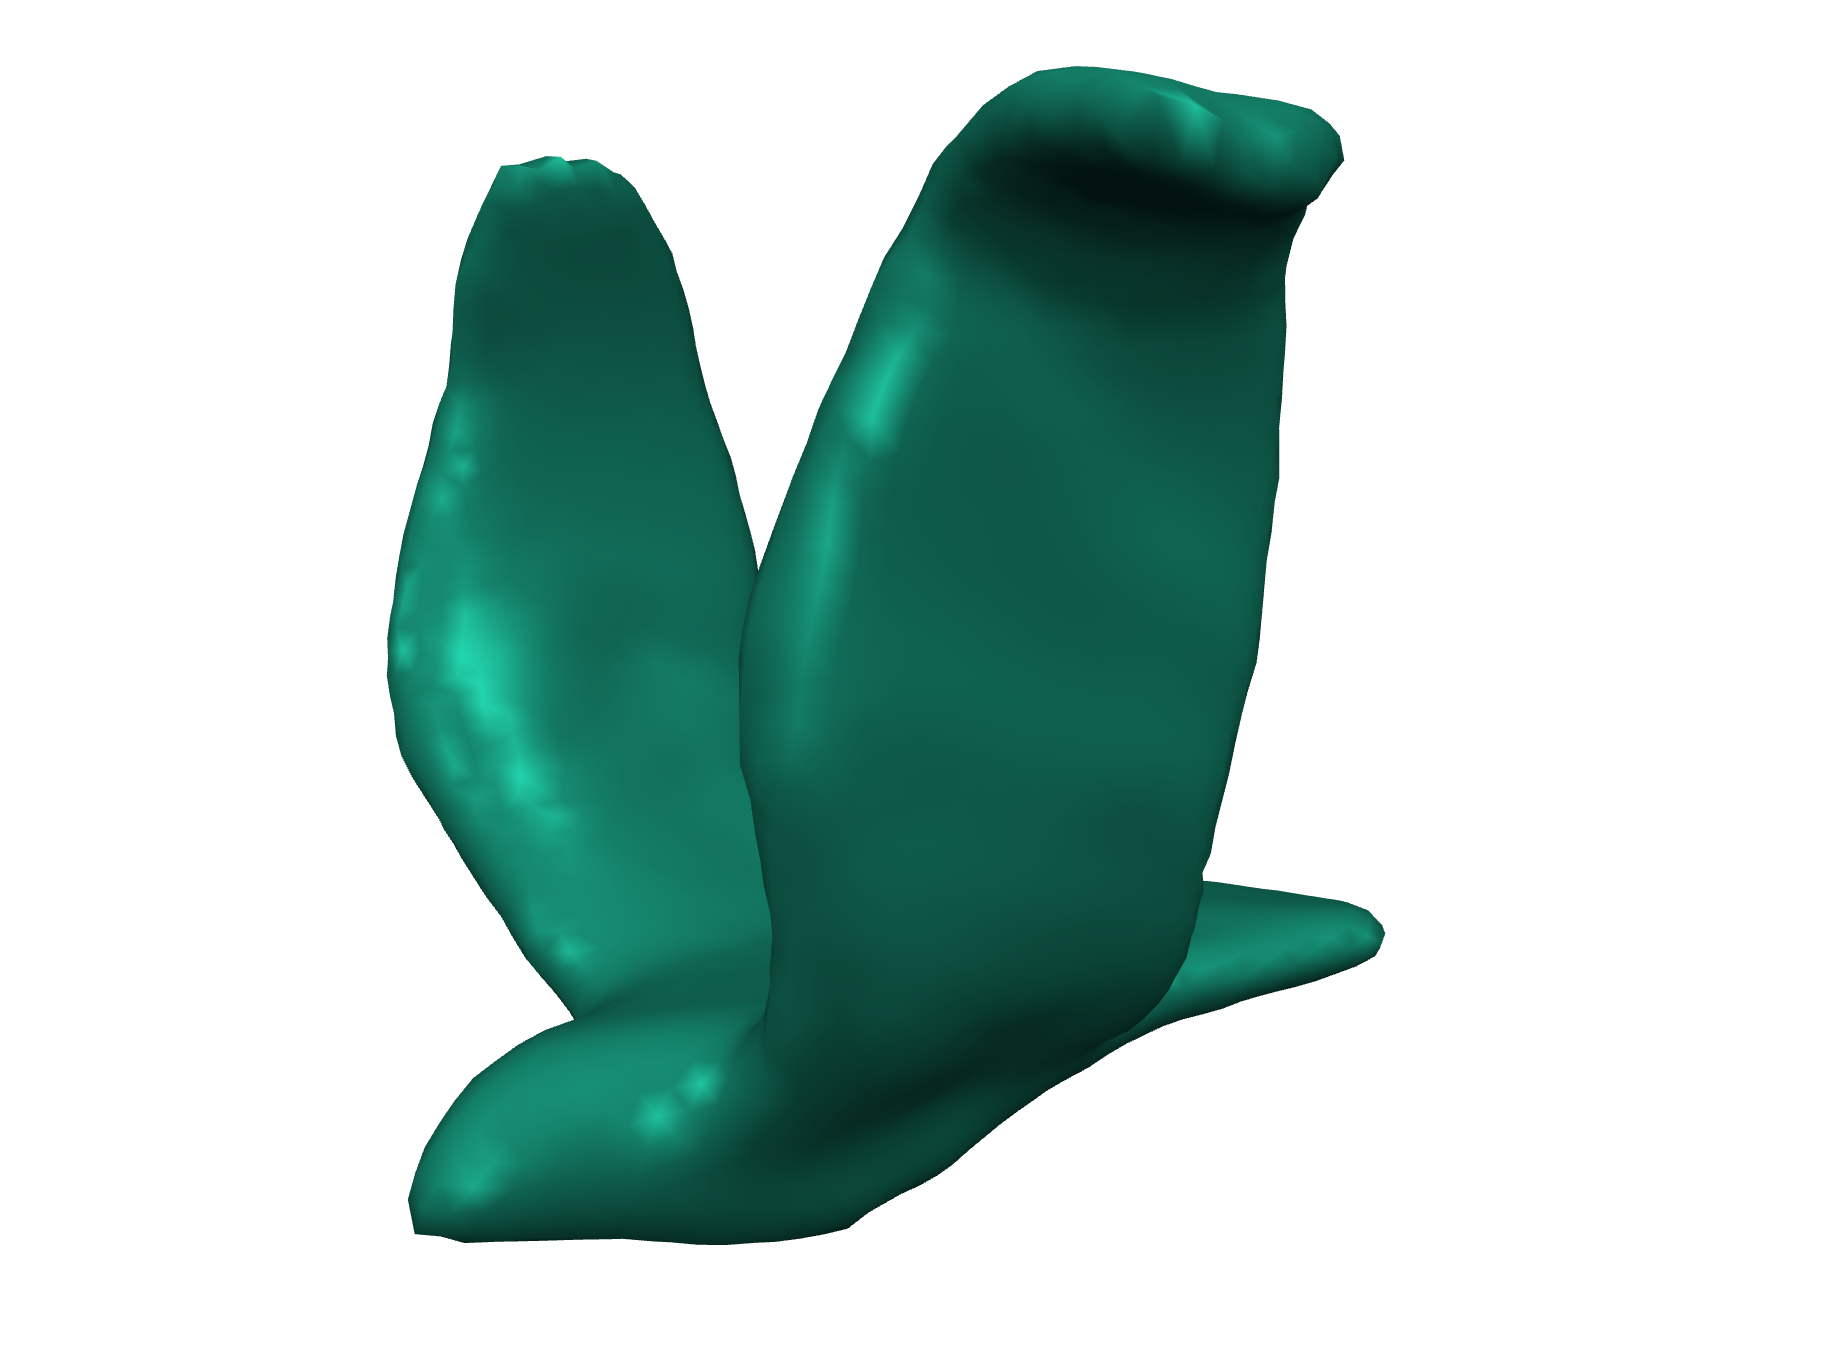
\includegraphics[width=0.44\textwidth]{resources/bent_side1.png} 
    \caption{Side view of bent object}
    \label{fig:bird_deformed_bend_side}
\end{figure}

For both cases, the results are good, and no artefacts can be seen. With these experiments, we can conclude that the energy behaves well even for larger, more complex meshes. In addition, we have now seen different deformations than just the stretching along one axis of the object, and the energy was able to handle these configurations. That suggests that the energy is suited for arbitrary deformations on arbitrary meshes.

\section{Optimization}
\label{s:optimization}
In order to achieve realistic results, we not only need to choose a suitable model but also an appropriate algorithm to get the exact solution or a satisfying approximation within a reasonable amount of time. For the performed simulations, a standard Newton solver augmented with a line search was used. Linear systems were solved by using conjugate gradient implementation. This section gives an overview of these methods.

\subsection{Newton's Method}
The task of the optimization, in this case, is to find an acceptable minimum of the strain energy after changing the boundary conditions. We can formulate this problem more generally as
\[
	\text{minimize} \quad f(x): \mathbb{R}^n \rightarrow \mathbb{R}.
\]
In order to find a minimum, the condition $\nabla f(x) = 0$ has to be satisfied. 
For solving this problem, we can use Newton's method, which iteratively approaches an acceptable minimum. To achieve this, we need to know the correct search direction to approach a minima step by step. The search direction is given by the Newton step, which uses the second derivative of the function $f$:
\[
	\nabla x_{nt} := - \nabla^2 f(x)^{-1} \nabla f(x)
\]
Now we need to know how much we can move in this direction. The line search algorithm can answer this question. It outputs the maximum amount to move in a given search direction. Newton's method can be very fast compared to other methods and produces a solution of high accuracy. The main disadvantage is that the calculation and storage of the second derivative and computing the Newton step can be quite costly (\cite{boyd2004convex}, p. 484-487, 496). Thus, the analysis of the Hessian of the deformation energy was a necessary step to show that the energy is suited for practical applications.

\subsection{Conjugate Gradient}
The conjugate gradient method is an algorithm that solves a system of linear equations. We can write the problem generally as
\[
	\mathbf{A}\mathbf{x} = \mathbf{k},
\]
where $\mathbf{A}$ is a symmetric, positive definite ($n \times n$)-matrix. Both $\mathbf{A}$ and $\mathbf{k}$ are known. The conjugate gradient method delivers an approximation of the exact solution within a certain tolerance. It iteratively searches for an appropriate $\mathbf{x}$, starting with an initial estimate. It usually reaches convergence fast and is computationally efficient (\cite{hestenes1952methods}, p. 409-412). In the code, the conjugate gradient method was used iteratively with the help of the library Eigen, which has already implemented the corresponding functionalities.

\section{Discussion}
The authors of the paper \acrshort{snh} introduced a novel hyperelastic model for the deformation energy. My first approach for this thesis was to dive into the topic of flesh simulation. The most important topics concerning this learning process are introduced and explained in \autoref{c:Background}. The next step was to understand and being able to explain the thought process of the authors. The paper itself can be a bit complicated for somebody who does not yet have a broad knowledge of the field. I documented this step in \autoref{c:Paper}. In the same chapter, it also appears to be clear why a new energy formulation was necessary. None of the existing energies satisfied all of the requirements stated in \autoref{ss:stability}. Some of them even produced severe artefacts or could not preserve the volume. Finally, I conducted some experiments on my own to verify some of the author's claims. The implementation the authors provided helped me during this process, not only for the simulations but also to get a better understanding of the energy. In \autoref{c:Experiments}, I first experimented with different values for the Poisson's ratio and was able to verify the claim that the model behaves well for a wide range of Poisson's ratio, even for one close to 0.5. In addition, I could recreate some other examples they covered in their paper. For each simulation included in this thesis, the model satisfies the requirements the authors listed without the need of using filter parameters. Furthermore, the scramble test validates the robustness of the model, and the deformations on the bird mesh suggest that the energy is suited for arbitrary deformations on arbitrary meshes. But in order to make a final statement of the quality of the energy, it would be necessary to make more specific tests, for example, the behaviour of a hand or an arm. In addition, the results should be compared with the ones produced from other energy formulations, similar to some of the tests the authors included in their paper. Unfortunately, this would have been beyond the scope of this thesis. From the findings I could require during my thesis, it nonetheless appears that there is a great improvement in the quality of the simulation with this new energy model for materials with a high Poisson's ratio.
